\documentclass{cmspaper}

\usepackage{amsfonts,amsmath,amssymb}
\usepackage{slashed}
\usepackage{bm}
\usepackage{appendix}
\usepackage[dvips]{graphicx}
\usepackage[a4paper]{hyperref}

% necessary in order to have boldmath in section titles and hyperref not crashing
\DeclareBoldMathCommand{\bE}{E}
\DeclareBoldMathCommand{\bp}{p}

\begin{document}

%==============================================================================
% title page for few authors

\begin{titlepage}

% select one of the following and type in the proper number:
%  \cmsnote{2005/000}
   \internalnote{2009/007}
%  \conferencereport{2005/000}
%  \cmsan{2005/000}
%  \cmsdtnote{2005/000}
%  \cmspas{2005/000}
%  \cmsnote{2009/XXX}
\date{31 January 2009}

\title{Study of Impact of HO on Jet Reconstruction}

\begin{Authlist}
  Sarah Eno, Dinko Ferencek
     \Instfoot{umd}{University of Maryland, College Park, MD, USA}
\end{Authlist}


\begin{abstract}
A study of impact of HO on jet reconstruction with the CMS detector is presented. For this purpose a sample of full simulation single-jet events has been produced and analyzed. At the focus of the study was the jet transverse energy resolution. The study shows that inclusion of HO in jet reconstruction leads to small improvements in jet transverse energy resolution and reduces the effects of energy leakage, especially in the most central $\eta$ region where Ring $0$ is located. However, overall improvement in jet transverse energy resolution is relatively small and it does not exceed $1\%$. 
\end{abstract} 

  
\end{titlepage}

\setcounter{page}{2}%JPP


\section{Introduction}

The hadron outer (HO) calorimeter~\cite{ref:cms-jinst} is the outermost component of the CMS hadronic calorimeter (HCAL) and is located outside the magnet coil. Its primary purpose is to increase the effective thickness of the hadronic calorimeter in the barrel region ($|\eta|<1.3$) and thus to identify late starting showers leaking outside the hadron barrel calorimeter (HB) and sample their energy. This ``tail-catching'' property of HO should improve the overall hermetic design of the CMS detector and reduce the tails in the energy resolution function, thus leading to more accurate measurements of the jet transverse energy, $E_\mathrm{T}$, and of the missing transverse energy, $\slashed E_\mathrm{T}$.

The HO design is constrained by the geometry of the muon system. HO covers the region $|\eta|<1.26$ and consists of five separate rings ($0$,$\pm 1$,$\pm 2$). The central ring (Ring $0$) has two scintillator layers on either side of the iron absorber while all other rings have only one scintillator layer on the outer side of the iron absorber. The position of HO scintillator layers in the overall CMS design is shown in Fig.~\ref{fig:HO_layers}. HO scintillators follow the HB tower geometry in $\eta$ and $\phi$. Approximate dimensions along $\eta$ of different HO rings are given in Table~\ref{tab:ring_dim}.
\begin{table}[h]
 \caption{Approximate dimensions along $\eta$ of different HO rings.}
 \centering
 \begin{tabular}{c|c}
  Ring    & Dimension along $\eta$ \\ \hline \hline
  $0$     & $|\eta|\lesssim0.33$ \\ \hline
  $\pm 1$ & $0.33\lesssim|\eta|\lesssim 0.86$ \\ \hline
  $\pm 2$ & $0.86\lesssim|\eta|\lesssim 1.26$
 \end{tabular}
 \label{tab:ring_dim}
\end{table}

\begin{figure}[b]
 \centering
 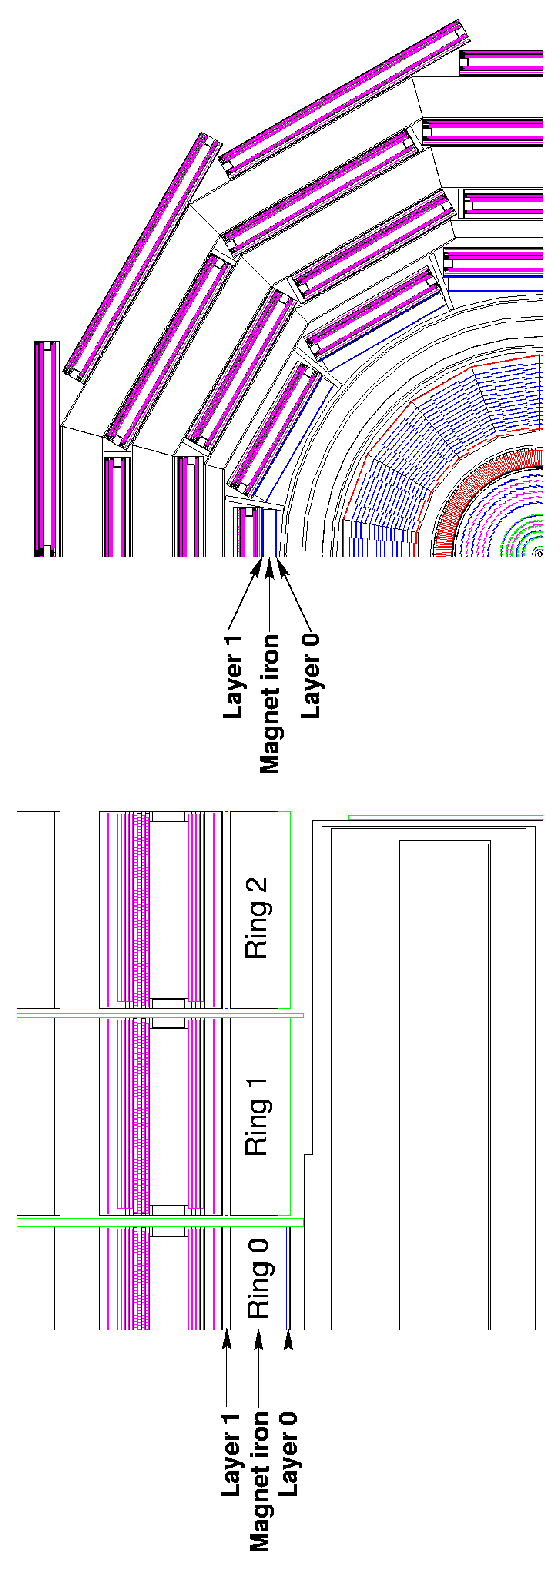
\includegraphics[angle=-90,width=0.95\textwidth]{fig/HO_layers}
 \caption{Longitudinal and transverse views of the CMS detector showing the position of HO scintillator layers.}
 \label{fig:HO_layers}
\end{figure}

With the release of \texttt{IDEAL\_V9} global tag for conditions data~\cite{ref:frontier}, HO went from the least noisy HCAL subdetector to the noisiest HCAL subdetector. This prompted its removal from the default jet reconstruction sequence starting from CMSSW\_2\_1\_8~\cite{ref:cmssw}. This, however, might have some unwanted consequences on the reconstruction of jets and missing transverse energy such as reduced energy resolution. 

This note is organized as follows. Simulated data as well as jet selection criteria used in this study are described in Section~\ref{sc:mc_samples}. Analysis procedure and obtained results are presented in Section~\ref{sc:results}. Finally, short summary and conclusions are given in Section~\ref{sc:summary}.


\section{Monte Carlo Samples}
\label{sc:mc_samples}

A sample of full simulation single-jet events was generated using CMSSW\_2\_1\_8 and P\textsc{ythia} version 6.416 in particle gun mode. Generated jets were originating from the initial $d$-quark generated with the transverse momenta of $p_\mathrm{T}=50$, $100$, $300$, $500$, $1000$, $2000$, $4000$, and $7000$ GeV$/c$ and with pseudorapidities of $\eta=0.1$, $0.5$, and $1.0$. $\eta$ values were chosen so that most of the HO energy would come from only one HO ring. 6 000 events were generated for each pair of values of transverse momentum $p_\mathrm{T}$ and pseudorapidity $\eta$, i.e., 144 000 events in total. \texttt{IDEAL\_V9} global tag for conditions data was used. 

In order to study the impact of HO on jet reconstruction, \texttt{iterativeCone5} jet algorithm was used to reconstruct both generator level jets (GenJets) and calorimeter level jets (calojets). \texttt{iterativeCone5} calojets were reconstructed with HO contribution (CaloJetsWithHO) and without HO contribution (CaloJets) included in the jet reconstruction. HO threshold used in calorimeter tower (CaloTower) reconstruction was changed from its default Scheme B~\cite{ref:scheme_b} value of 1.1 GeV to 2.2 GeV. Reason for this increase in threshold is higher level of noise in HO introduced with \texttt{IDEAL\_V9} detector conditions for which default Scheme B threshold was not optimized~\cite{ref:thresh}. Additional effect that had to be corrected for is the ECAL cell saturation bug~\cite{ref:ecal_cell} for which only a partial fix was available at the time of writing this note.

\subsection{Jet Selection Criteria}

In this particular analysis there is exactly one generated GenJet per event and the only selection criterion required was that GenJets have $p_\mathrm{T}>30$ GeV$/c$. Similarly, for calojets the only selection criterion was that they have $p_\mathrm{T}>15$ GeV$/c$. After GenJets and calojets had been selected, they were matched using One-To-One matching tool~\cite{ref:one_to_one}. Some of the obtained kinematic distributions for GenJets and calojets are given in Appendix~\ref{app:kin_dist}. $p_\mathrm{T}$ spectra of the GenJet constituent particles are given in Appendix~\ref{app:pT_spect}.


\section{Results}
\label{sc:results}

As it was already mentioned, \texttt{iterativeCone5} calojets were reconstructed with and without HO contribution included. It is then expected that the difference between CaloJetWithHO energy ($E^\text{calo, HO}$) and CaloJet energy ($E^\text{calo}$) in the same event would almost entirely come from the HO energy contribution. This is confirmed in Fig.~\ref{fig:h_DeltaE_EHO} where a clear correlation between the calojet energy difference ($E^\text{calo, HO}-E^\text{calo}$) and HO energy contribution (\texttt{hadEnergyInHO}) taken from CaloJetWithHO can be observed. Correlation between HO and HB energy contributions for CaloJetsWithHO for different values of parton $\eta$ is shown in Fig.~\ref{fig:h_EHO_EHB}. As expected, correlation is stronger for lower values of $\eta$ where the effective thickness of HB is smaller.

\begin{figure}
 \centering
 \begin{tabular}{lll}
  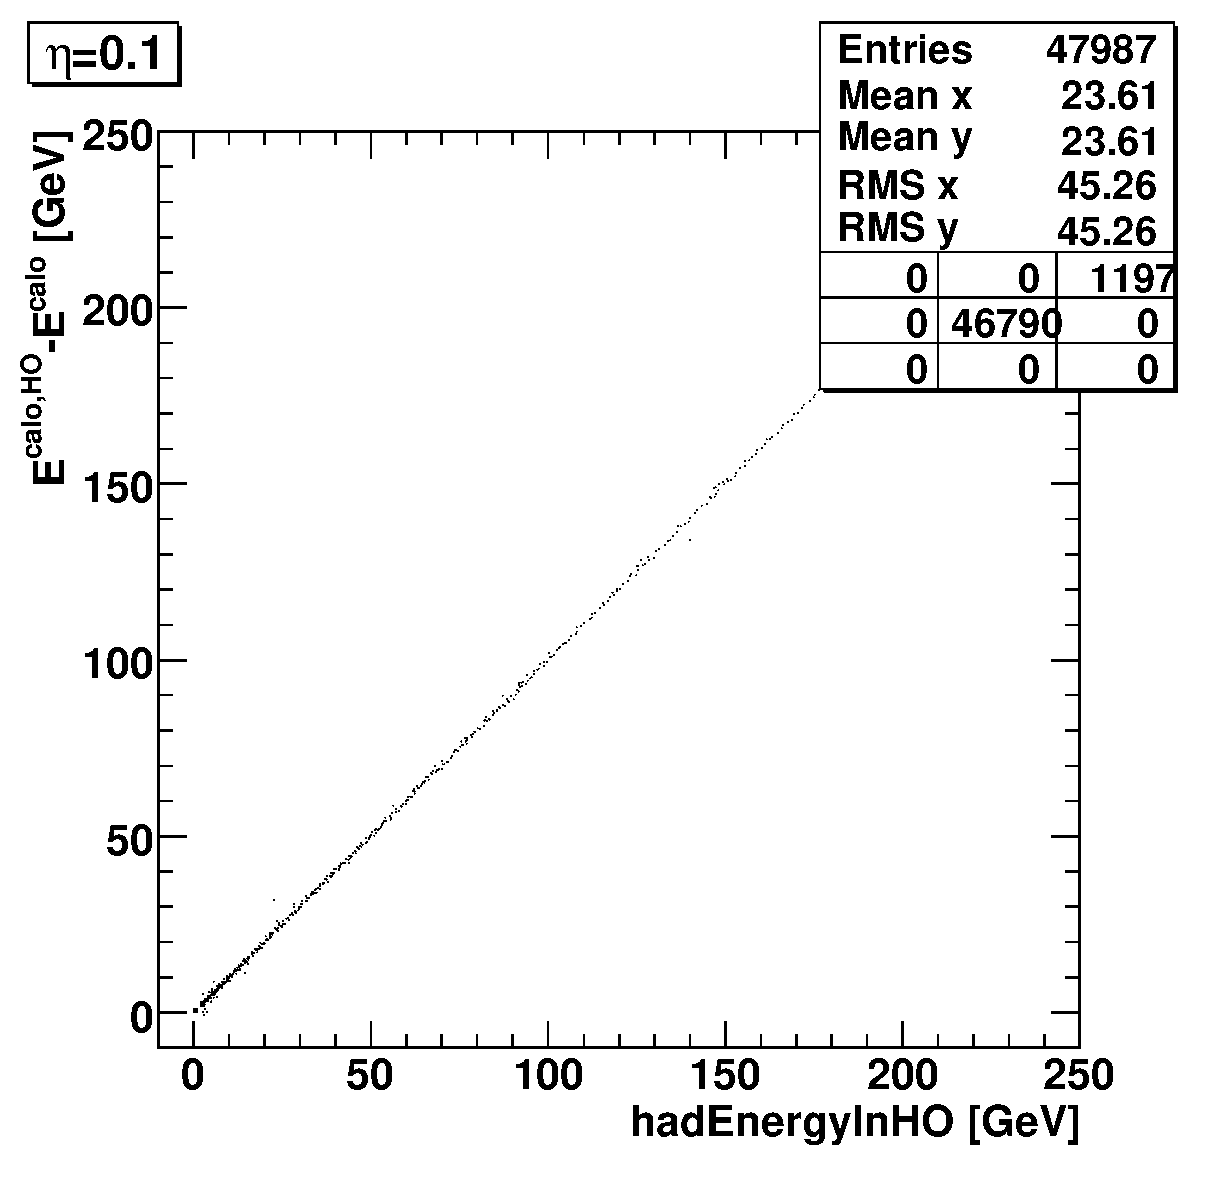
\includegraphics[width=0.31\textwidth]{fig/h_DeltaE_EHO_corr_eta0.1.eps} &
  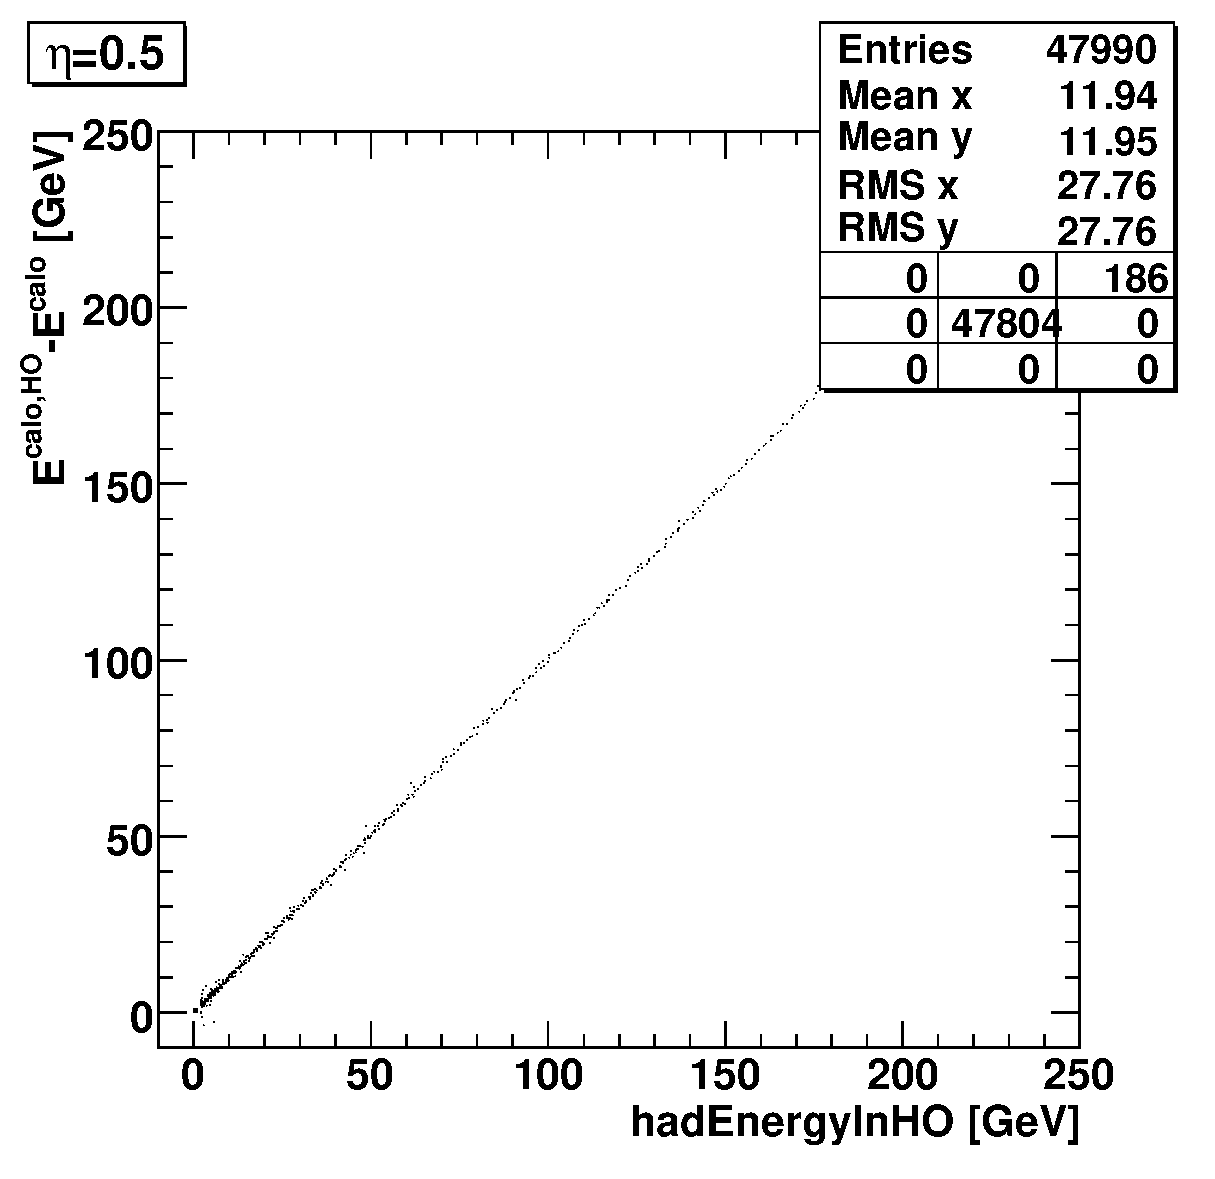
\includegraphics[width=0.31\textwidth]{fig/h_DeltaE_EHO_corr_eta0.5.eps} &
  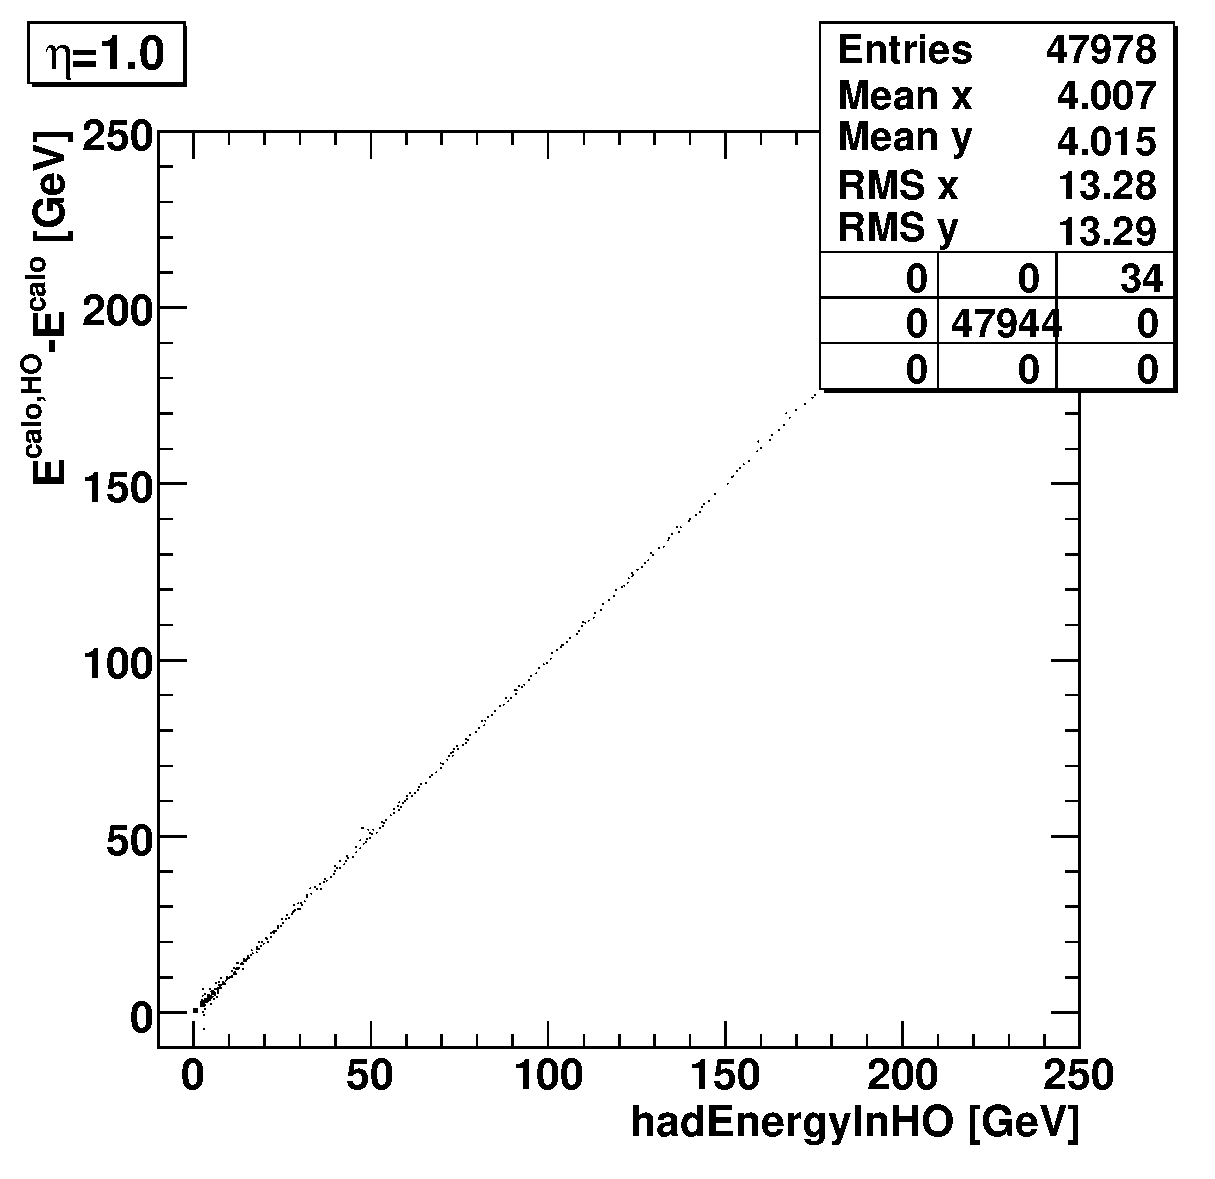
\includegraphics[width=0.31\textwidth]{fig/h_DeltaE_EHO_corr_eta1.0.eps} \\
 \end{tabular}
 \caption{Difference between CaloJetWithHO energy and CaloJet energy ($E^\text{calo, HO}-E^\text{calo}$) in the same event vs. HO energy contribution (\texttt{hadEnergyInHO}) taken from CaloJetWithHO for parton $\eta=0.1$ (left), $0.5$ (center), and $1.0$ (right).}
 \label{fig:h_DeltaE_EHO}
\end{figure}

\begin{figure}
 \centering
 \begin{tabular}{lll}
  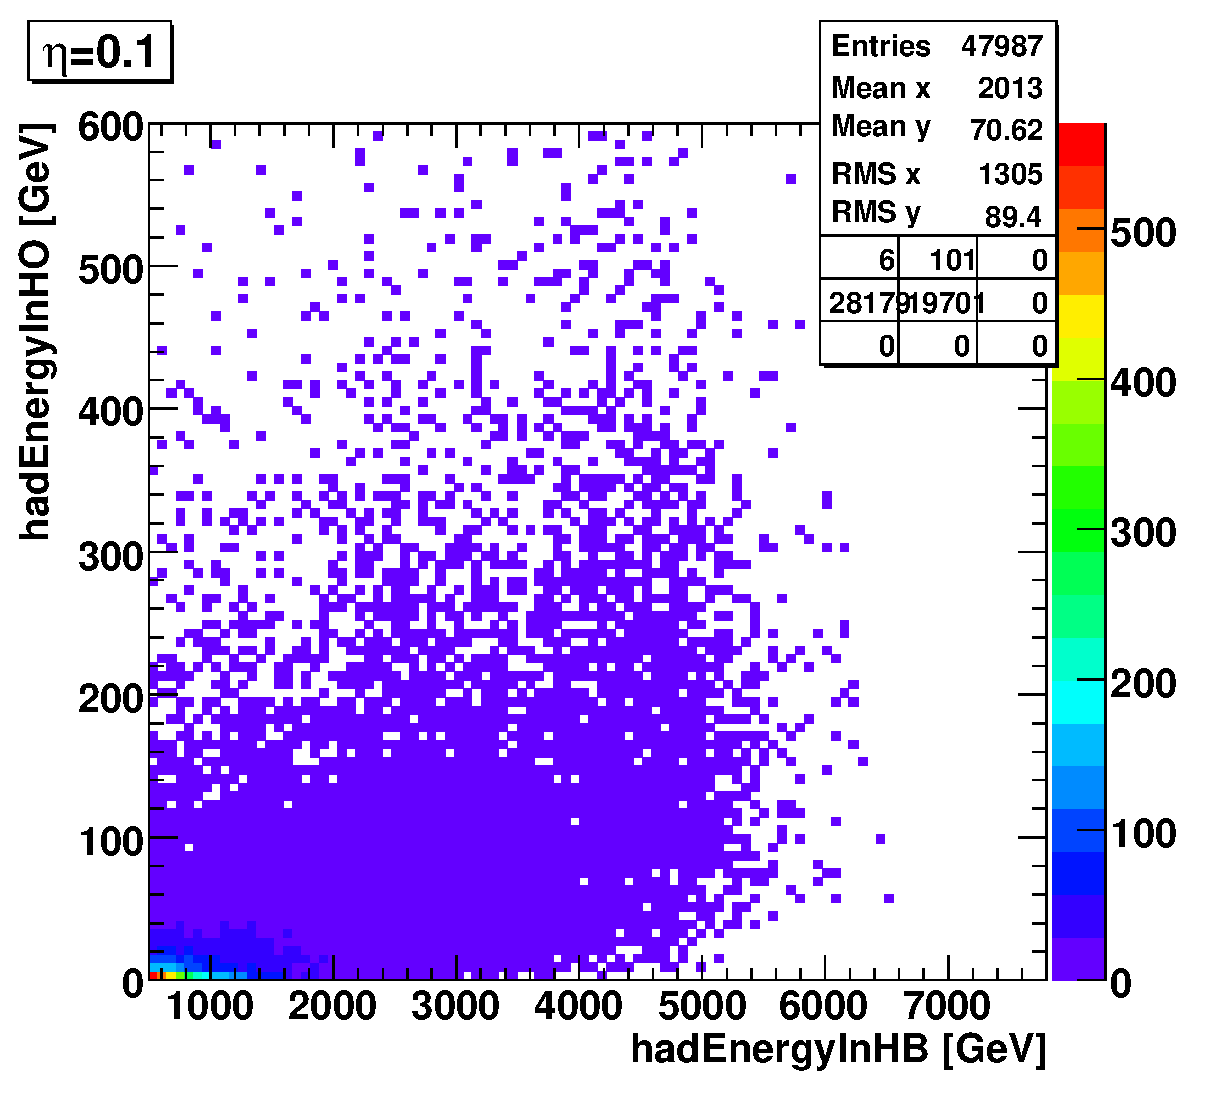
\includegraphics[width=0.31\textwidth]{fig/h_EHO_EHB_corr_eta0.1.eps} &
  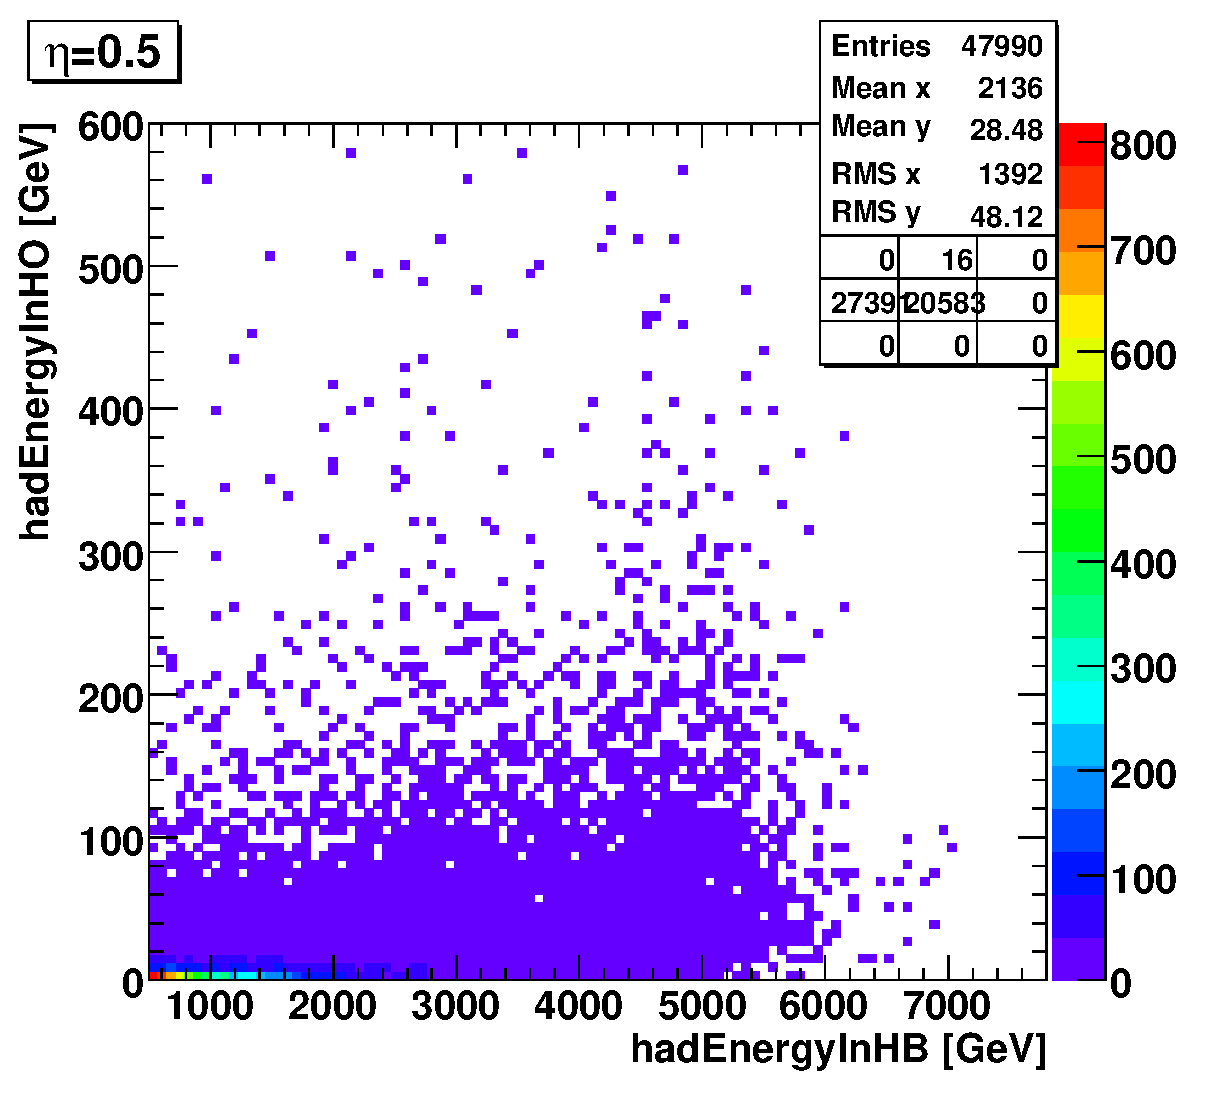
\includegraphics[width=0.31\textwidth]{fig/h_EHO_EHB_corr_eta0.5.eps} &
  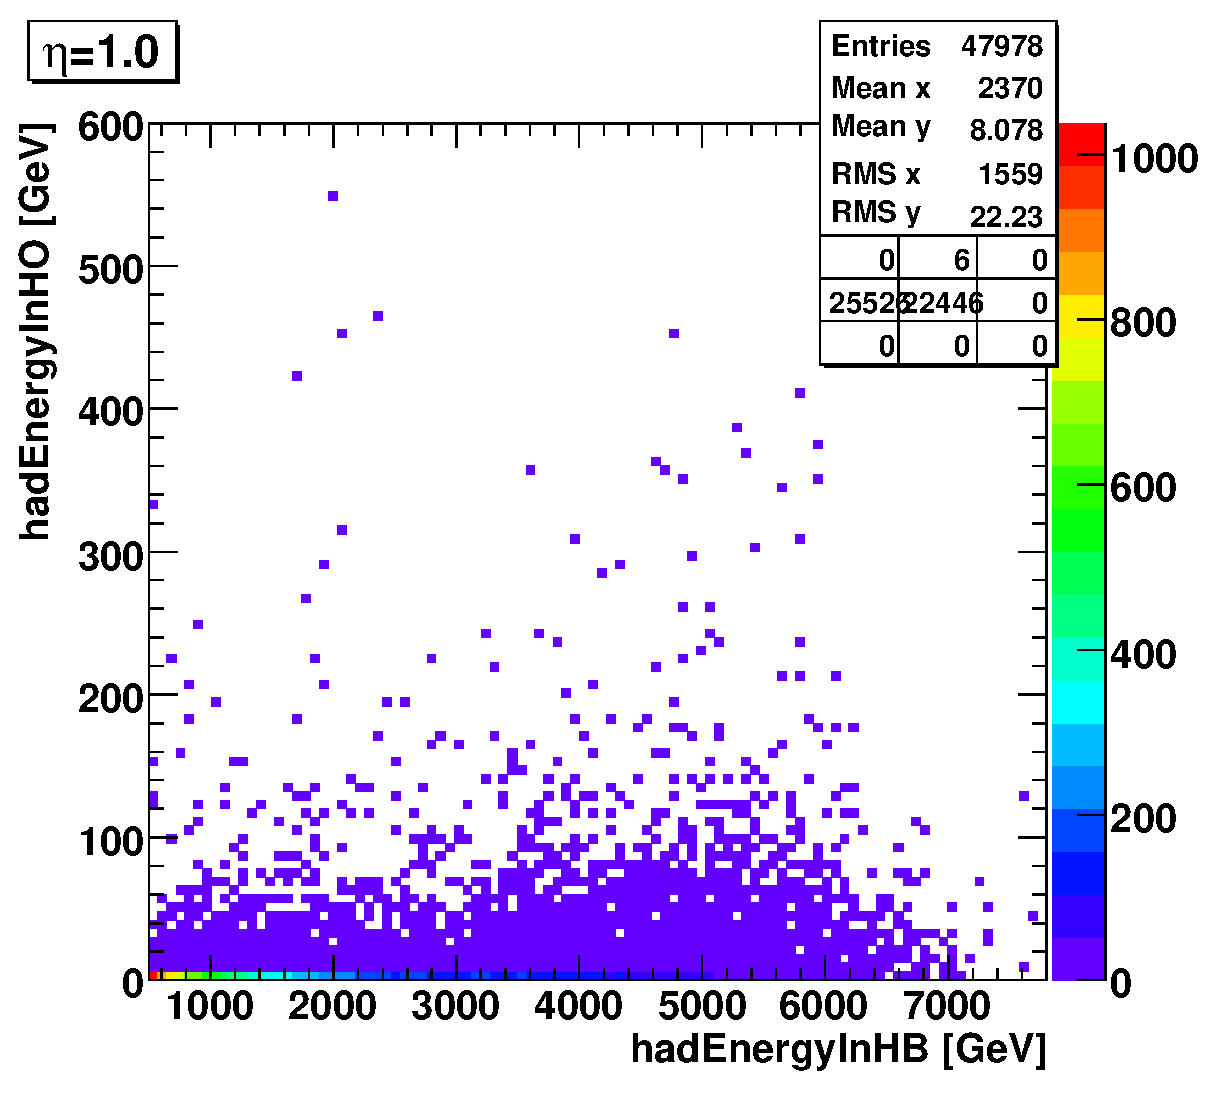
\includegraphics[width=0.31\textwidth]{fig/h_EHO_EHB_corr_eta1.0.eps} \\
 \end{tabular}
 \caption{Correlation between HO and HB energy contributions for CaloJetsWithHO for parton $\eta=0.1$ (left), $0.5$ (center), and $1.0$ (right).}
 \label{fig:h_EHO_EHB}
\end{figure}

Distributions from which all results were derived are $E^\text{calo}_\mathrm{T}/E^\text{gen}_\mathrm{T}$  and $E^\text{calo, HO}_\mathrm{T}/E^\text{gen}_\mathrm{T}$ distributions where $E^\text{calo}_\mathrm{T}$ ($E^\text{calo, HO}_\mathrm{T}$) and $E^\text{gen}_\mathrm{T}$ are transverse energies of the matched CaloJet (CaloJetWithHO) and GenJet, respectively. Obtained $E^\text{calo}_\mathrm{T}/E^\text{gen}_\mathrm{T}$ and $E^\text{calo, HO}_\mathrm{T}/E^\text{gen}_\mathrm{T}$ distributions for different values of parton $\eta$ are shown in Figures~\ref{fig:ETRatio_dist_01}, \ref{fig:ETRatio_dist_05}, and \ref{fig:ETRatio_dist_10}. As the $E^\text{gen}_\mathrm{T}$ increases, $E^\text{calo}_\mathrm{T}/E^\text{gen}_\mathrm{T}$ ($E^\text{calo, HO}_\mathrm{T}/E^\text{gen}_\mathrm{T}$) distributions move to the right and their mean values get closer to $1$, as expected. However, for $E^\text{gen}_\mathrm{T}\gtrsim2$ TeV mean values of the distributions start to decrease which is due to the fact that saturated ECAL cells even after correction still contain too little energy.
\begin{figure}
 \centering
 \begin{tabular}{ll}
  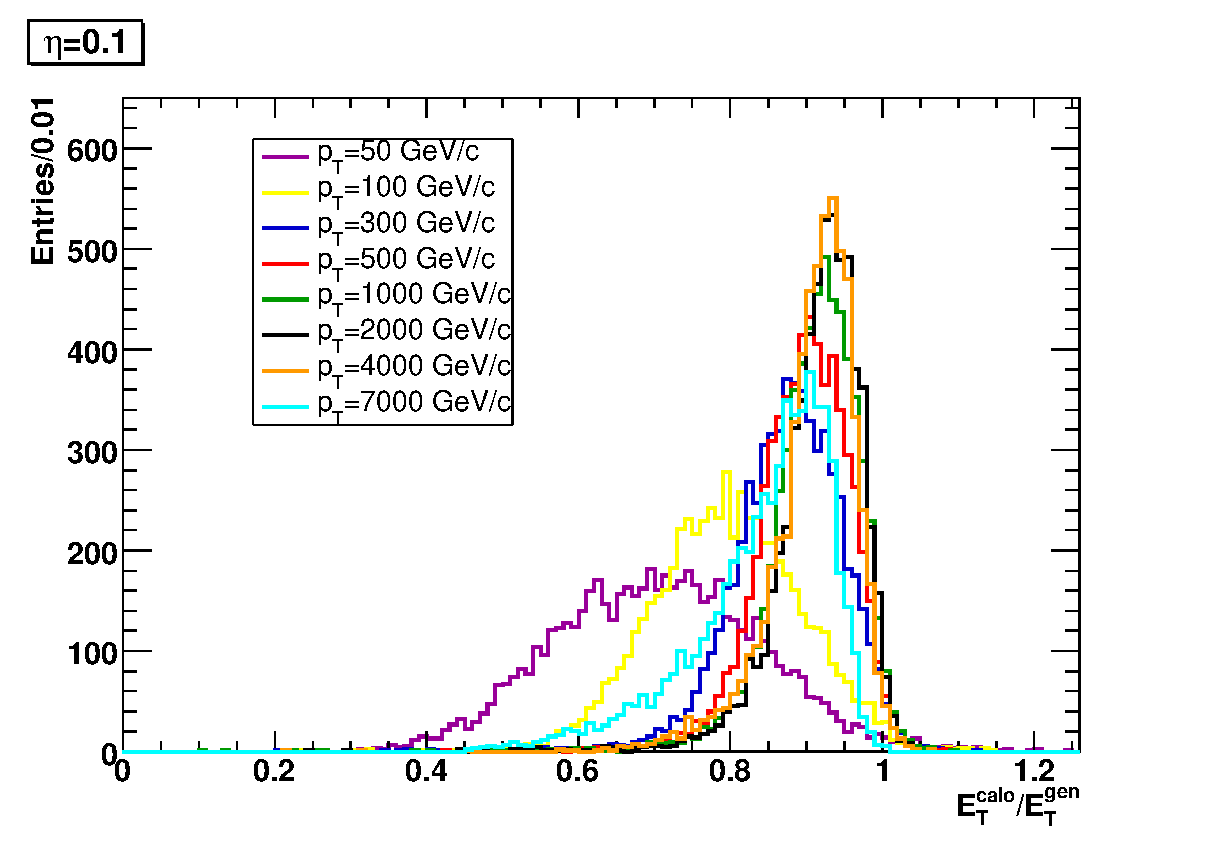
\includegraphics[width=0.5\textwidth]{fig/h_ETRatio_ET_py_corr_eta0.1.eps} &
  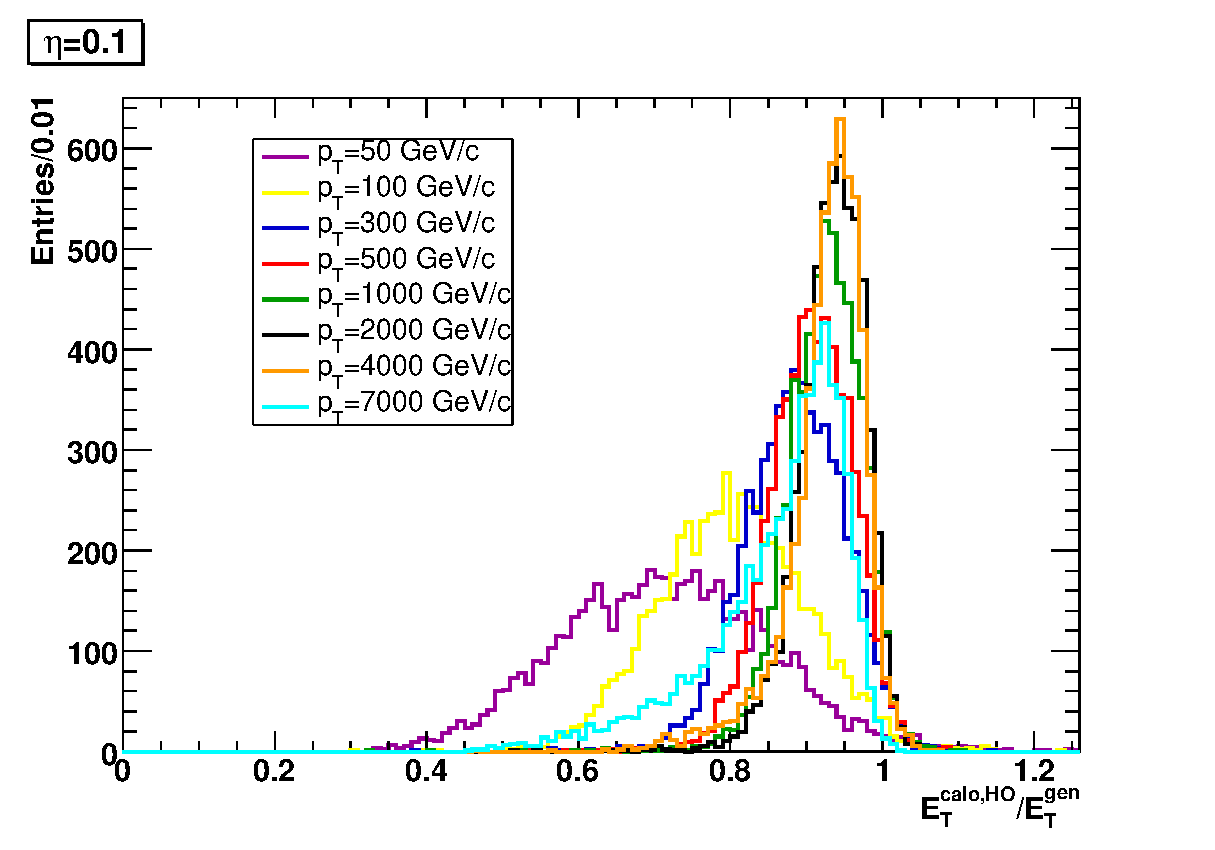
\includegraphics[width=0.5\textwidth]{fig/h_ETRatioWithHO_ET_py_corr_eta0.1.eps} \\
 \end{tabular}
 \caption{$E^\text{calo}_\mathrm{T}/E^\text{gen}_\mathrm{T}$ (left) and $E^\text{calo, HO}_\mathrm{T}/E^\text{gen}_\mathrm{T}$ (right) distributions for parton $\eta=0.1$.}
 \label{fig:ETRatio_dist_01}
\end{figure}

\begin{figure}
 \centering
 \begin{tabular}{ll}
  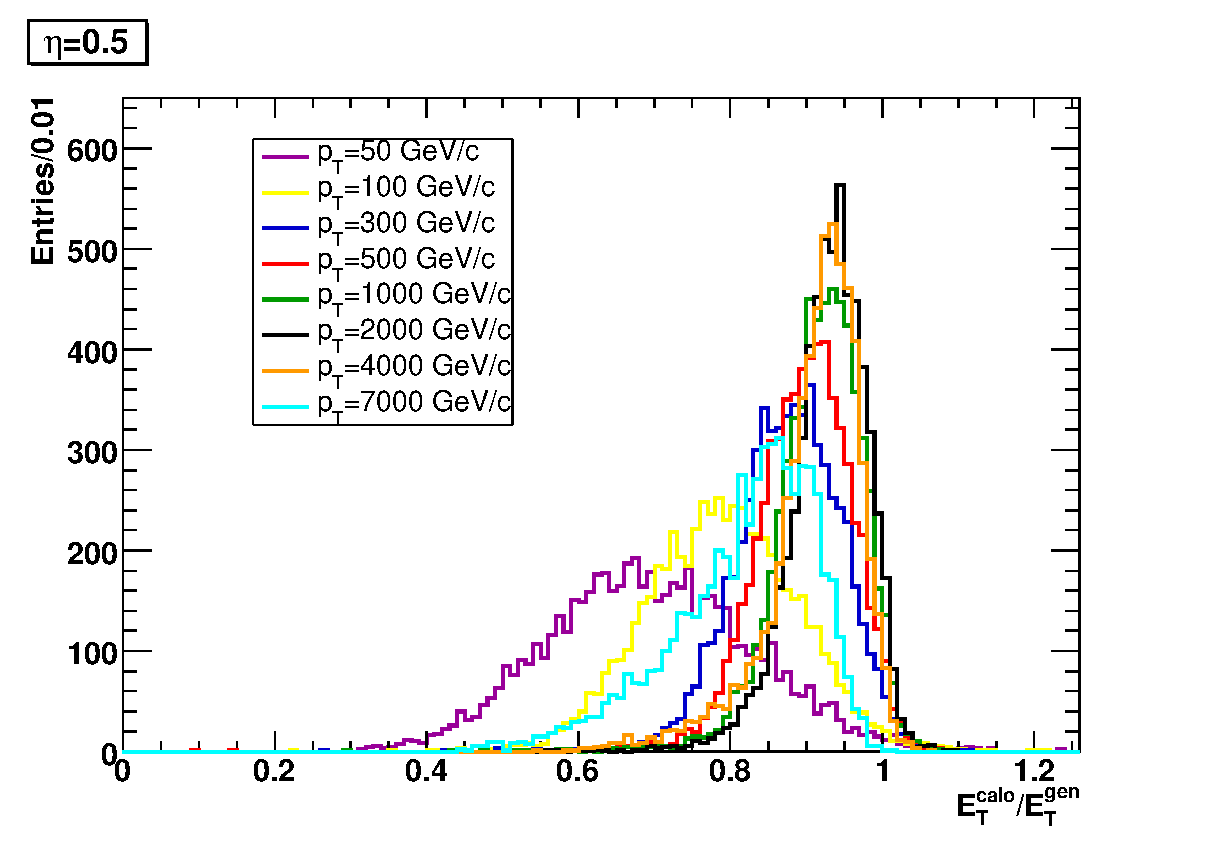
\includegraphics[width=0.5\textwidth]{fig/h_ETRatio_ET_py_corr_eta0.5.eps} &
  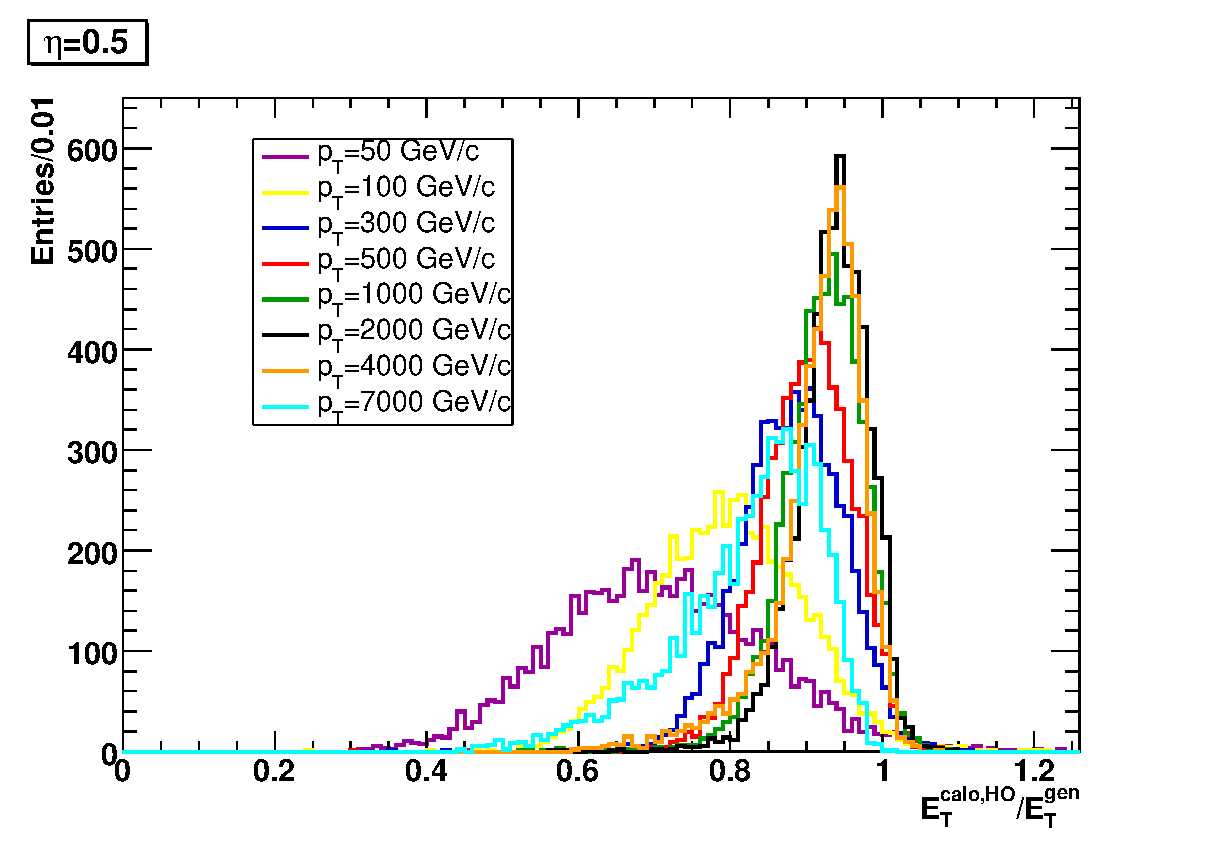
\includegraphics[width=0.5\textwidth]{fig/h_ETRatioWithHO_ET_py_corr_eta0.5.eps} \\
 \end{tabular}
 \caption{$E^\text{calo}_\mathrm{T}/E^\text{gen}_\mathrm{T}$ (left) and $E^\text{calo, HO}_\mathrm{T}/E^\text{gen}_\mathrm{T}$ (right) distributions for parton $\eta=0.5$.}
 \label{fig:ETRatio_dist_05}
\end{figure}

\begin{figure}
 \centering
 \begin{tabular}{ll}
  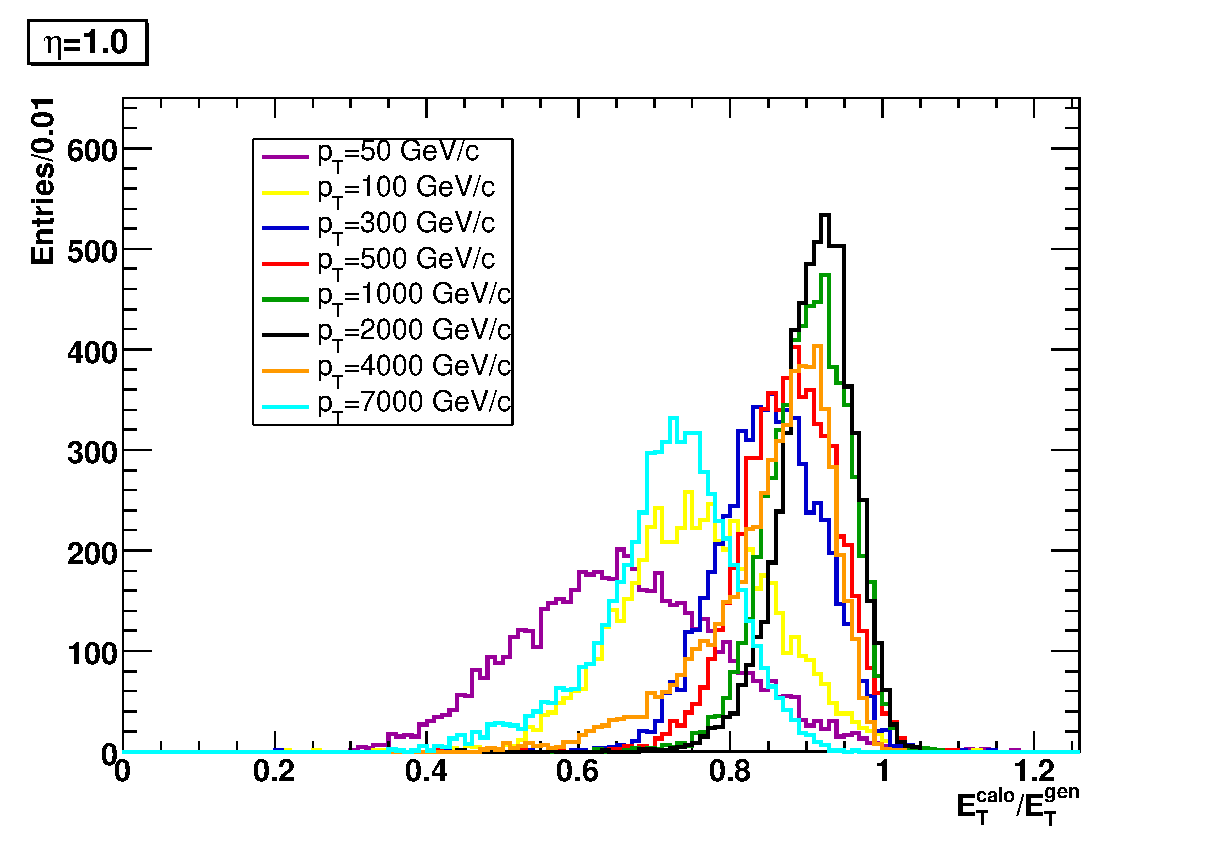
\includegraphics[width=0.5\textwidth]{fig/h_ETRatio_ET_py_corr_eta1.0.eps} &
  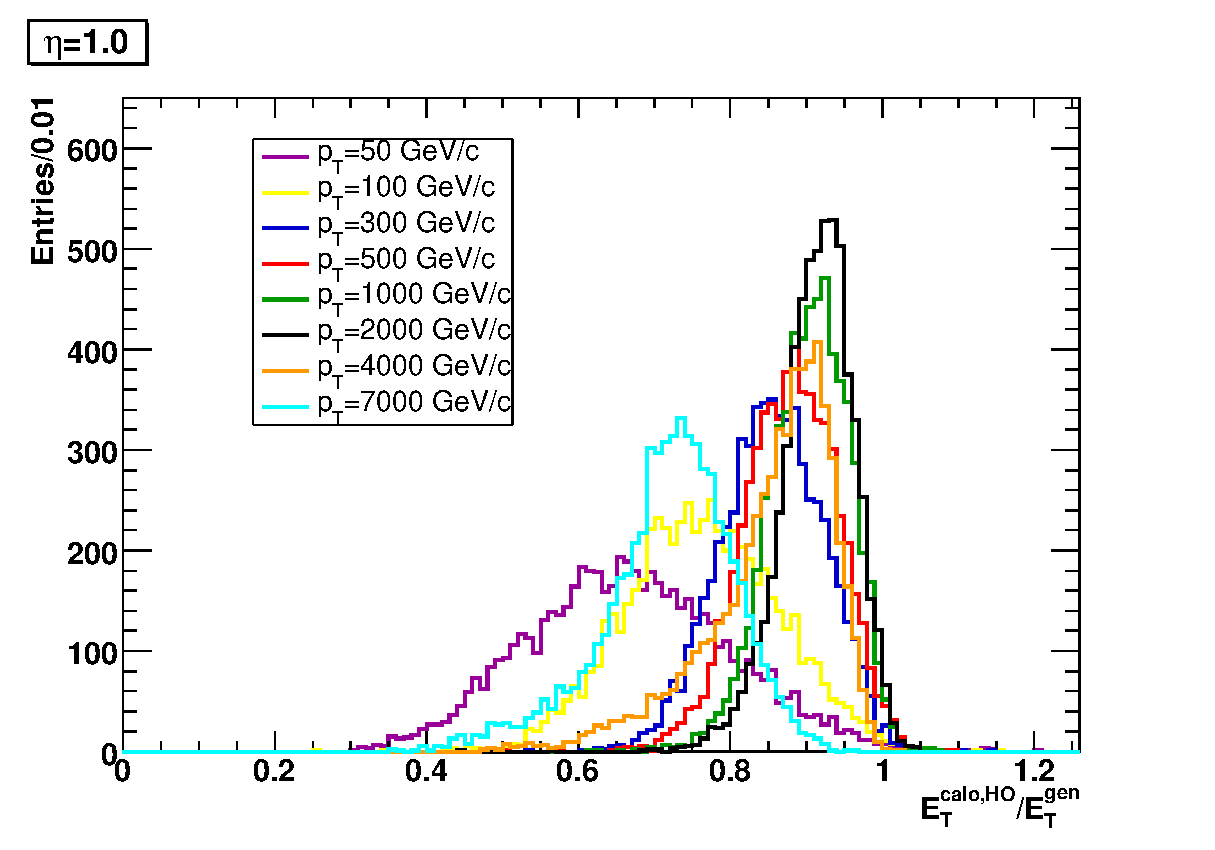
\includegraphics[width=0.5\textwidth]{fig/h_ETRatioWithHO_ET_py_corr_eta1.0.eps} \\
 \end{tabular}
 \caption{$E^\text{calo}_\mathrm{T}/E^\text{gen}_\mathrm{T}$ (left) and $E^\text{calo, HO}_\mathrm{T}/E^\text{gen}_\mathrm{T}$ (right) distributions for parton $\eta=1.0$.}
 \label{fig:ETRatio_dist_10}
\end{figure}

Quantity through which calojets with and without HO were compared is the jet $E_\mathrm{T}$ resolution. Jet $E_\mathrm{T}$ resolution is defined as
\begin{equation}
 \text{Jet }E_\mathrm{T}\text{ resolution}=\frac{\sigma\left(E^\text{calo}_\mathrm{T}/E^\text{gen}_\mathrm{T} \right)}{<E^\text{calo}_\mathrm{T}/E^\text{gen}_\mathrm{T}>},
\end{equation} 
where $\sigma\left(E^\text{calo}_\mathrm{T}/E^\text{gen}_\mathrm{T} \right)$ and $<E^\text{calo}_\mathrm{T}/E^\text{gen}_\mathrm{T}>$ are the standard deviation and the mean, respectively, of the Gaussian fit to $E^\text{calo}_\mathrm{T}/E^\text{gen}_\mathrm{T}$ distribution in $2\sigma$ region around the peak of the distribution. A full set of Gaussian fits to distributions shown in Figures~\ref{fig:ETRatio_dist_01}, \ref{fig:ETRatio_dist_05}, and \ref{fig:ETRatio_dist_10} is given in Appendix~\ref{app:fits}. By combining results from these fits, jet $E_\mathrm{T}$ resolution as a function of GenJet transverse energy $E^\text{gen}_\mathrm{T}$ was obtained and is shown in Figures~\ref{fig:ET_res_01}, \ref{fig:ET_res_05}, and \ref{fig:ET_res_10} for different values of parton $\eta$. From these plots it can be noticed that for calojets with HO contribution included, energy resolution gets slightly improved, most notably for very high energy jets in Ring $0$. However, overall improvement is still relatively small and it does not exceed $1\%$. For $E^\text{gen}_\mathrm{T}\gtrsim2$ TeV, energy resolution starts to degrade due to ECAL cell saturation bug.
\begin{figure}
 \centering
 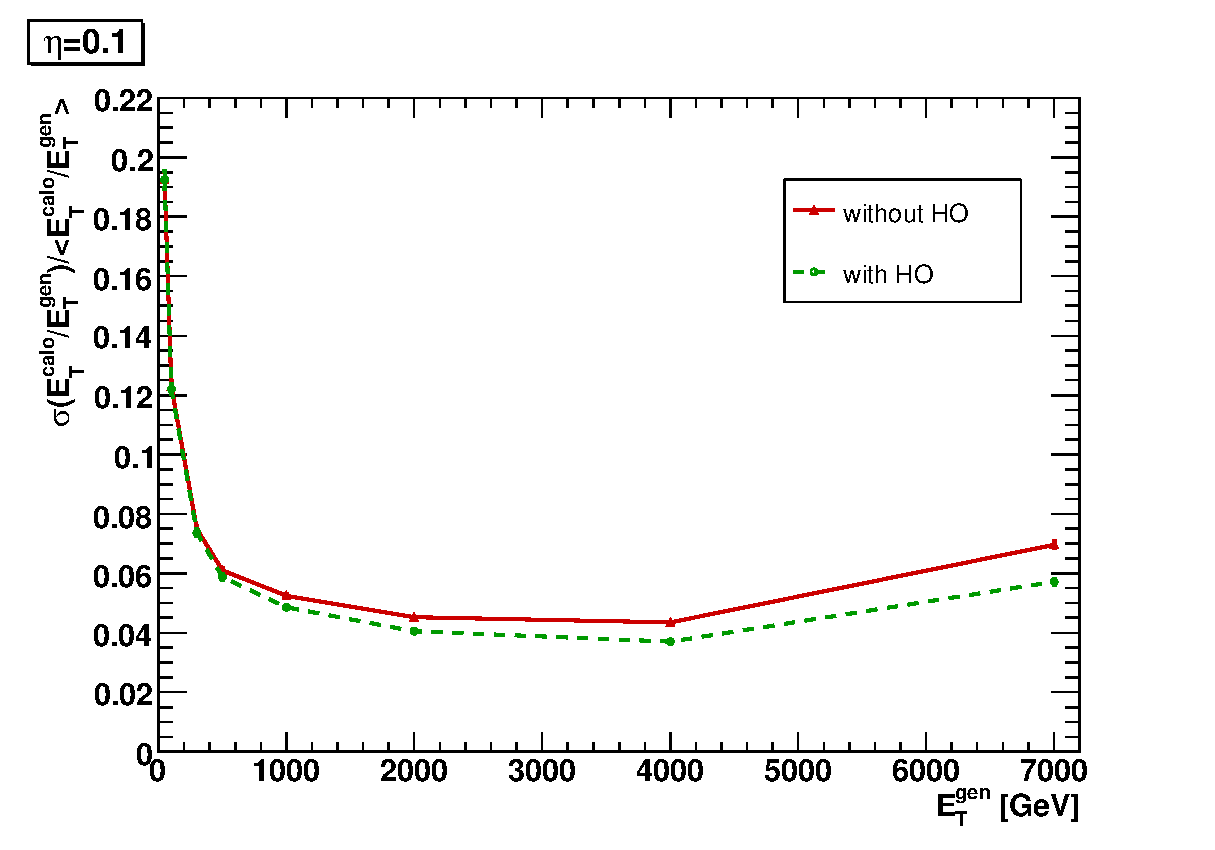
\includegraphics[width=0.66\textwidth]{fig/ET_resolution_corr_eta0.1.eps}
 \caption{Jet $E_\mathrm{T}$ resolution as a function of GenJet tranverse energy $E^\text{gen}_\mathrm{T}$ for parton $\eta=0.1$.}
 \label{fig:ET_res_01}
\end{figure}

\begin{figure}
 \centering
 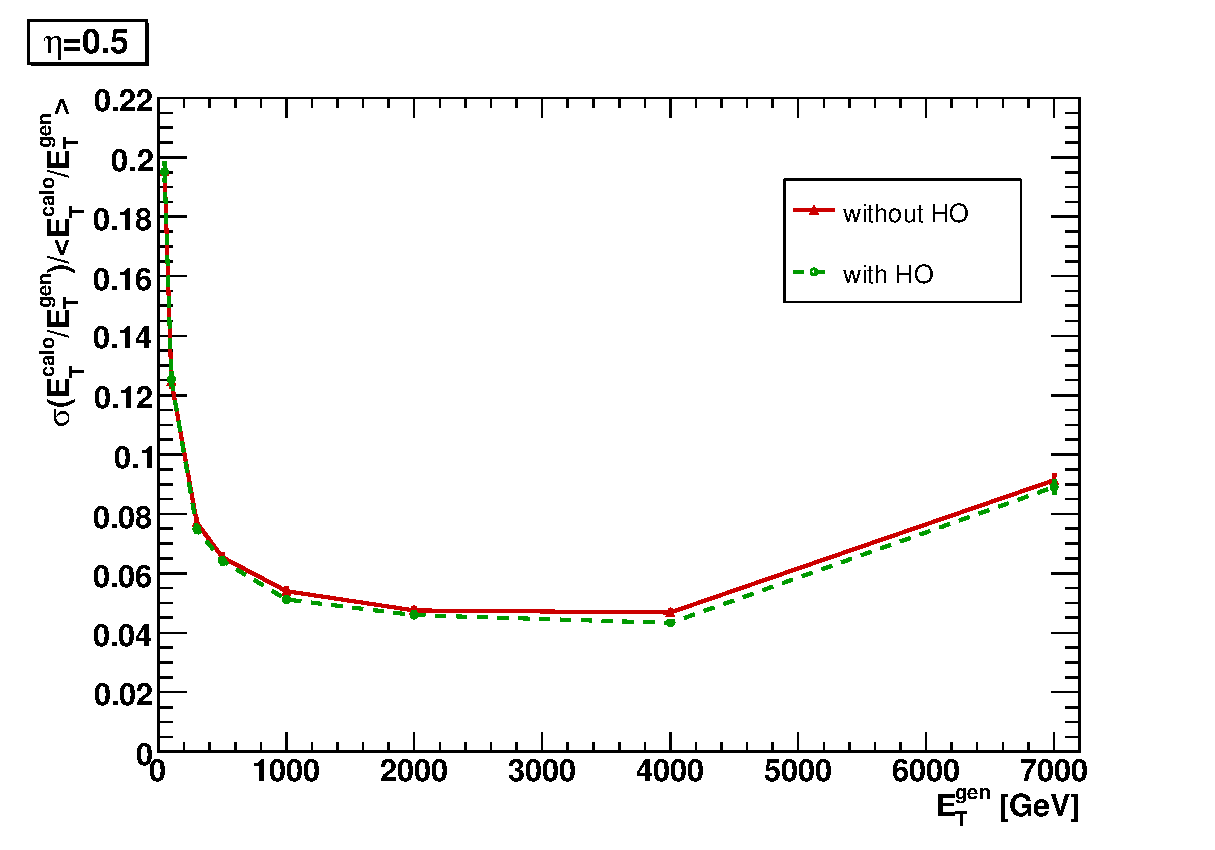
\includegraphics[width=0.66\textwidth]{fig/ET_resolution_corr_eta0.5.eps}
 \caption{Jet $E_\mathrm{T}$ resolution as a function of GenJet tranverse energy $E^\text{gen}_\mathrm{T}$ for parton $\eta=0.5$.}
 \label{fig:ET_res_05}
\end{figure}

\begin{figure}
 \centering
 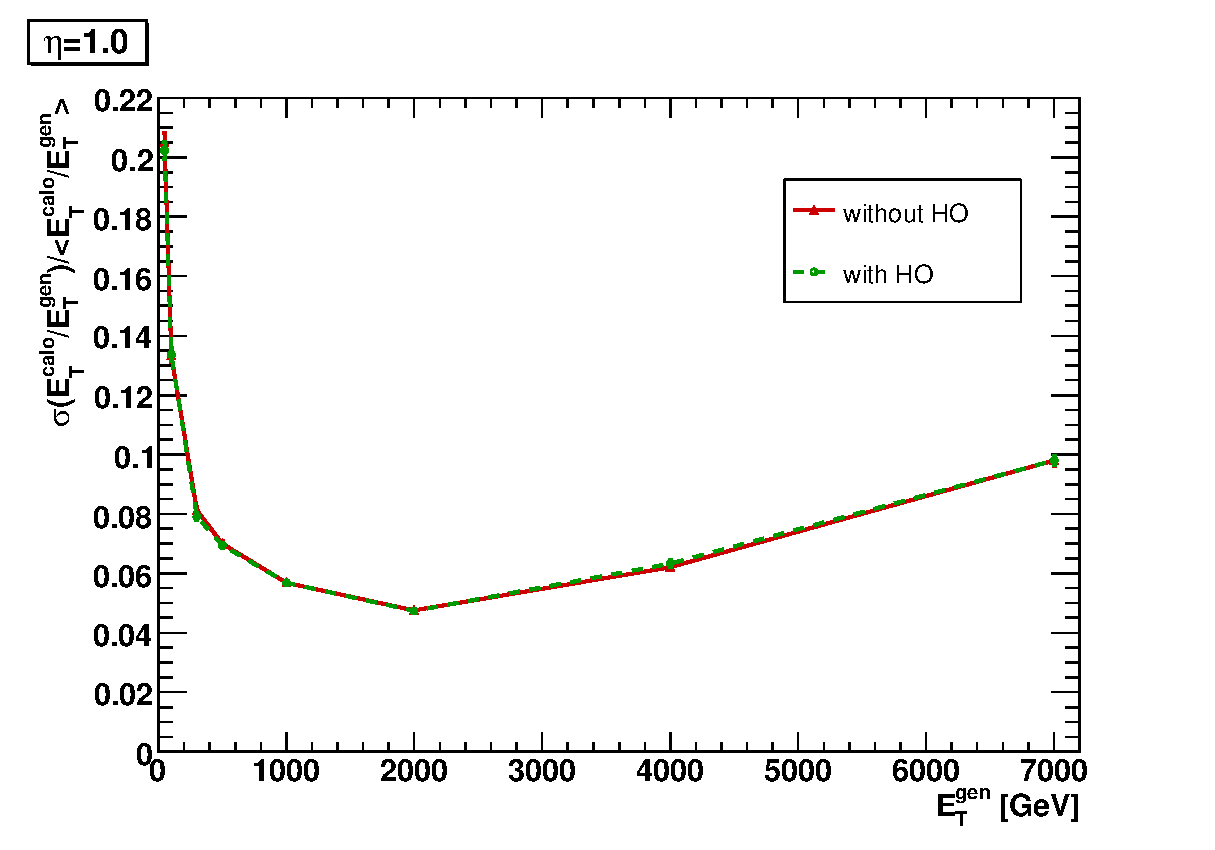
\includegraphics[width=0.66\textwidth]{fig/ET_resolution_corr_eta1.0.eps}
 \caption{Jet $E_\mathrm{T}$ resolution as a function of GenJet tranverse energy $E^\text{gen}_\mathrm{T}$ for parton $\eta=1.0$.}
 \label{fig:ET_res_10}
\end{figure}

Effect of energy leakage outside the HB can be studied by looking at the fraction of events with $E^\text{calo}_\mathrm{T}/E^\text{gen}_\mathrm{T}$ ($E^\text{calo, HO}_\mathrm{T}/E^\text{gen}_\mathrm{T}$) more than $3\sigma$ below the mean value. First thing to notice in Figure~\ref{fig:3sigma} is that any result for $E^\text{gen}_\mathrm{T}\gtrsim2$ TeV has to be discarded due to ECAL cell saturation bug. However, for $E^\text{gen}_\mathrm{T}\lesssim2$ TeV it can be seen that with HO included the 
fraction of events with significant leakage is kept below $\sim1.5\%$. Improvement is most significant for Ring $0$ while for Ring $2$ it practically vanishes. 
\begin{figure}
 \centering
 \begin{tabular}{lll}
  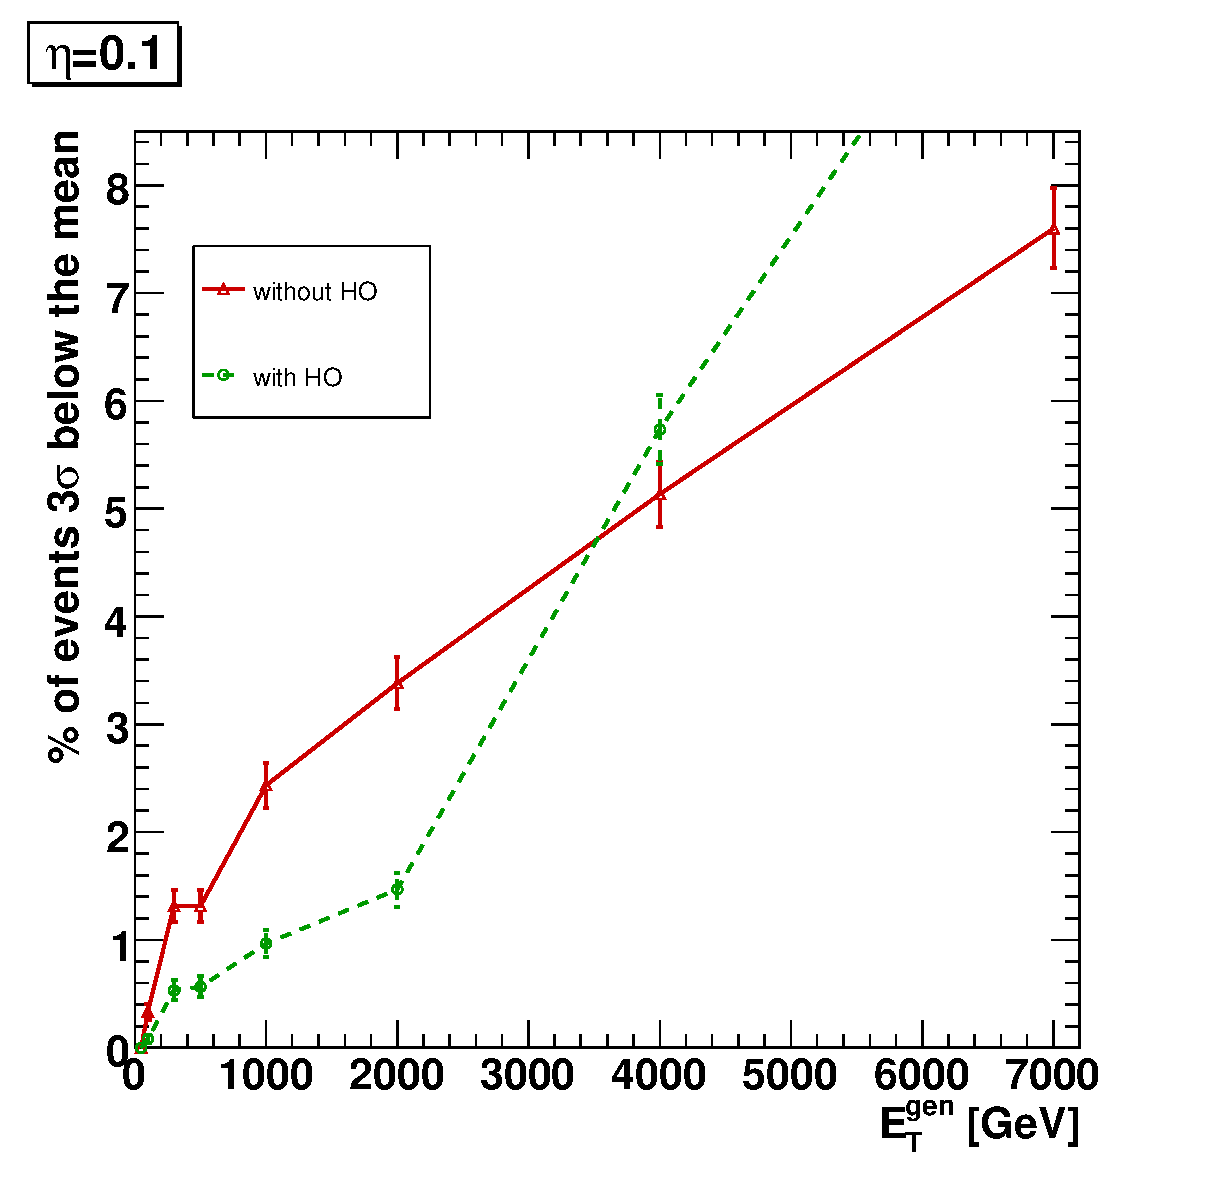
\includegraphics[width=0.31\textwidth]{fig/P3sigma_corr_eta0.1.eps} &
  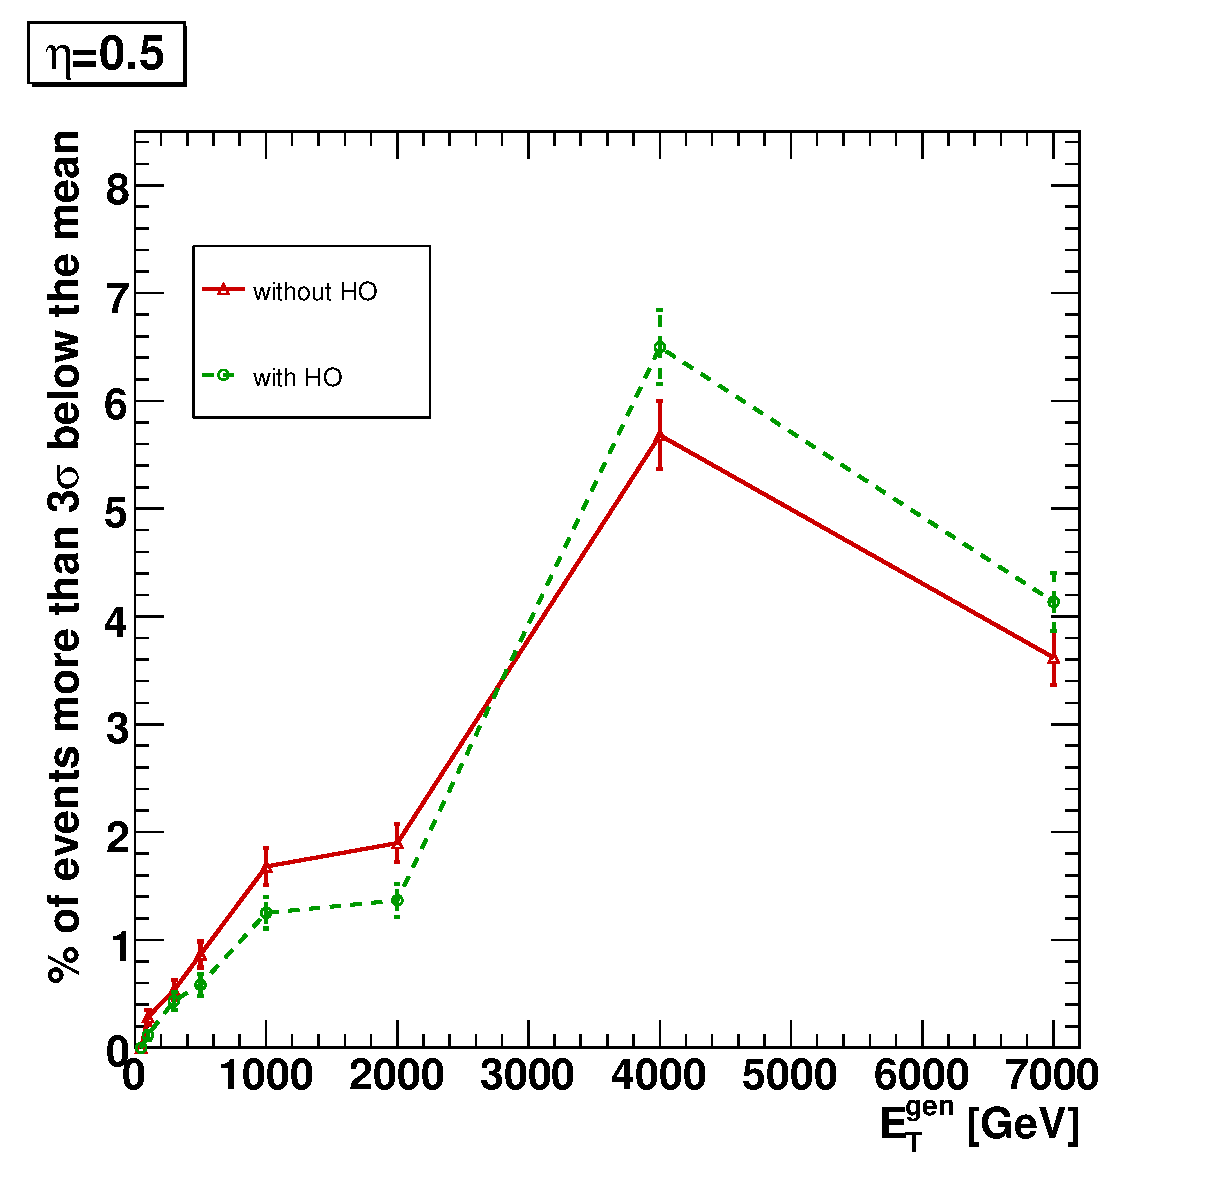
\includegraphics[width=0.31\textwidth]{fig/P3sigma_corr_eta0.5.eps} &
  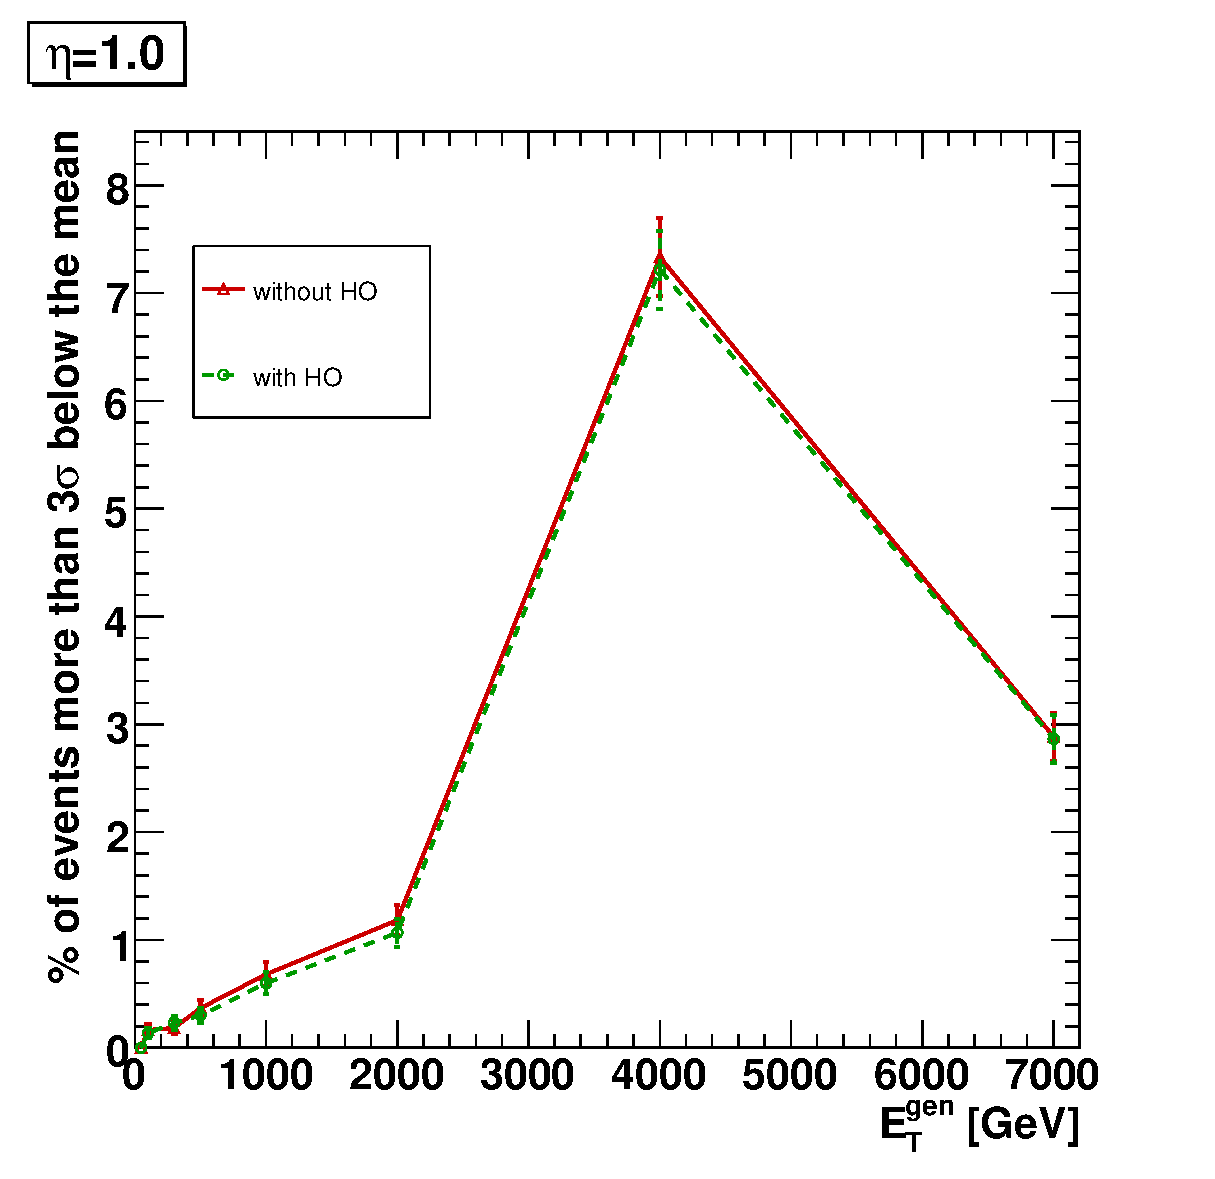
\includegraphics[width=0.31\textwidth]{fig/P3sigma_corr_eta1.0.eps} \\
 \end{tabular}
 \caption{Fraction of events with $E^\text{calo}_\mathrm{T}/E^\text{gen}_\mathrm{T}$ ($E^\text{calo, HO}_\mathrm{T}/E^\text{gen}_\mathrm{T}$) more than $3\sigma$ below the mean as a function of GenJet tranverse energy $E^\text{gen}_\mathrm{T}$ for parton $\eta=0.1$ (left), $0.5$ (center), and $1.0$ (right).}
 \label{fig:3sigma}
\end{figure}

Effect of adding HO energy contribution (\texttt{hadEnergyInHO}) with different weight factors on jet $E_\mathrm{T}$ resolution is illustrated in Appendix~\ref{app:res_vs_weight}.

\section{Summary}
\label{sc:summary}

A study of impact that HO has on jet reconstruction has been presented. Of particular interest are TeV jets where considerable amount of jet energy can leak outside HB. If HO is used in jet reconstruction, such energy leakages are taken into account and added to the total jet energy. This then improves accuracy of the jet energy measurements as well as measurements of the missing transverse energy.

Starting from CMSSW\_2\_1\_8 HO has been removed from the default jet reconstruction sequence to avoid introducing too much electronics noise into jet energy reconstruction. Main focus of this study was to compare jets reconstructed with and without HO contribution included. Obtained results show small improvements in jet transverse energy resolution when HO is included, especially in the most central $\eta$ region where Ring $0$ is located. However, overall improvement in jet transverse energy resolution is relatively small and it does not exceed $1\%$. Similarly, when HO is used, effects of energy leakage get reduced, especially in the most central $\eta$ region.

Finally, it can be concluded that the impact of HO on jet reconstruction is most significant in the most central $\eta$ region where the effective thickness of the hadronic calorimeter is at its minimum and HB cannot efficiently contain all the energy of very energetic jets. Further out in $\eta$ space, however, HB has sufficient thickness to efficiently contain even the most energetic jets. Therefore, it is more important to include in jet reconstruction those HO rings that are more central (Ring $0$ and Rings $\pm 1$) than those that are further out in $\eta$ (Rings $\pm 2$).


\begin{appendices}

\section{Kinematic Distributions for GenJets and CaloJets}
\label{app:kin_dist}

\begin{center}
 \begin{tabular}{lll}
  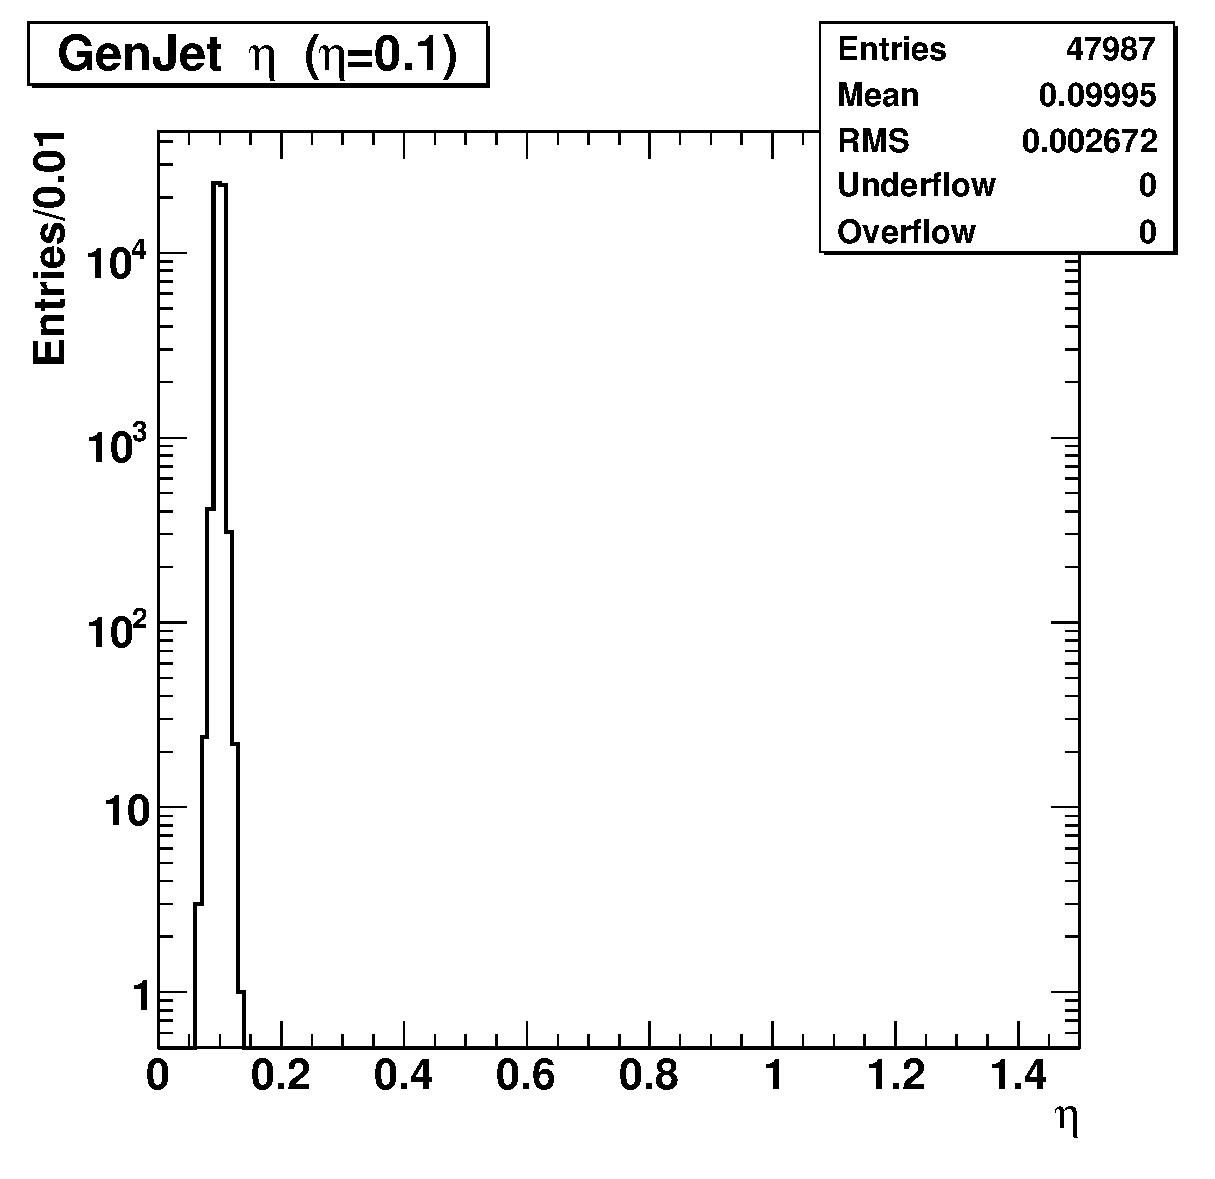
\includegraphics[width=0.31\textwidth]{fig/h_GenJetEta_corr_eta0.1.eps} &
  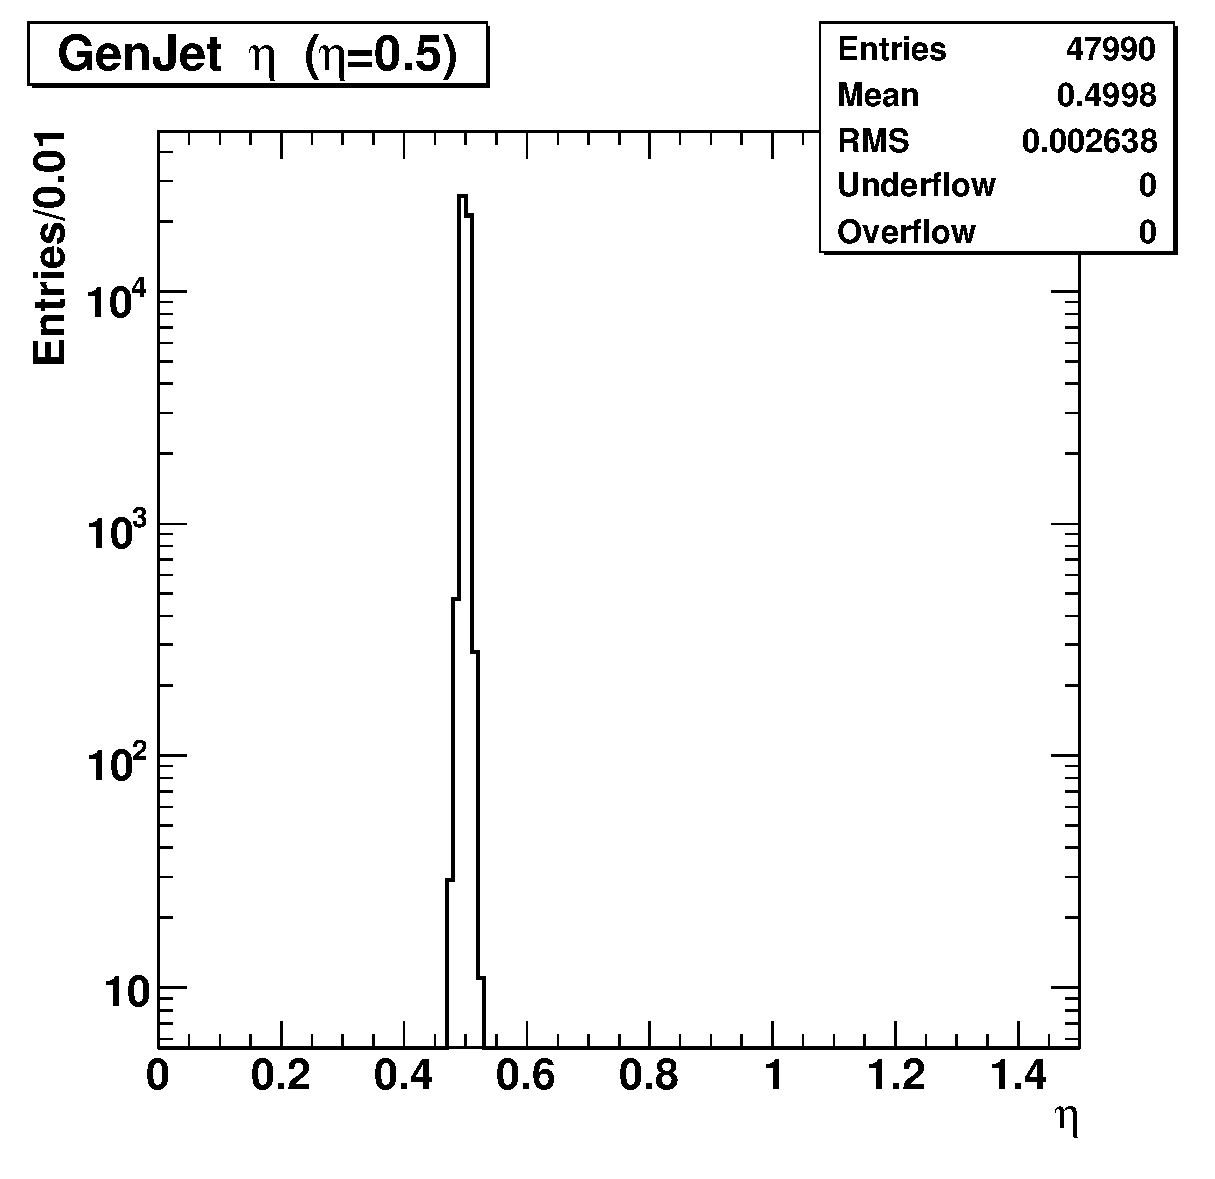
\includegraphics[width=0.31\textwidth]{fig/h_GenJetEta_corr_eta0.5.eps} &
  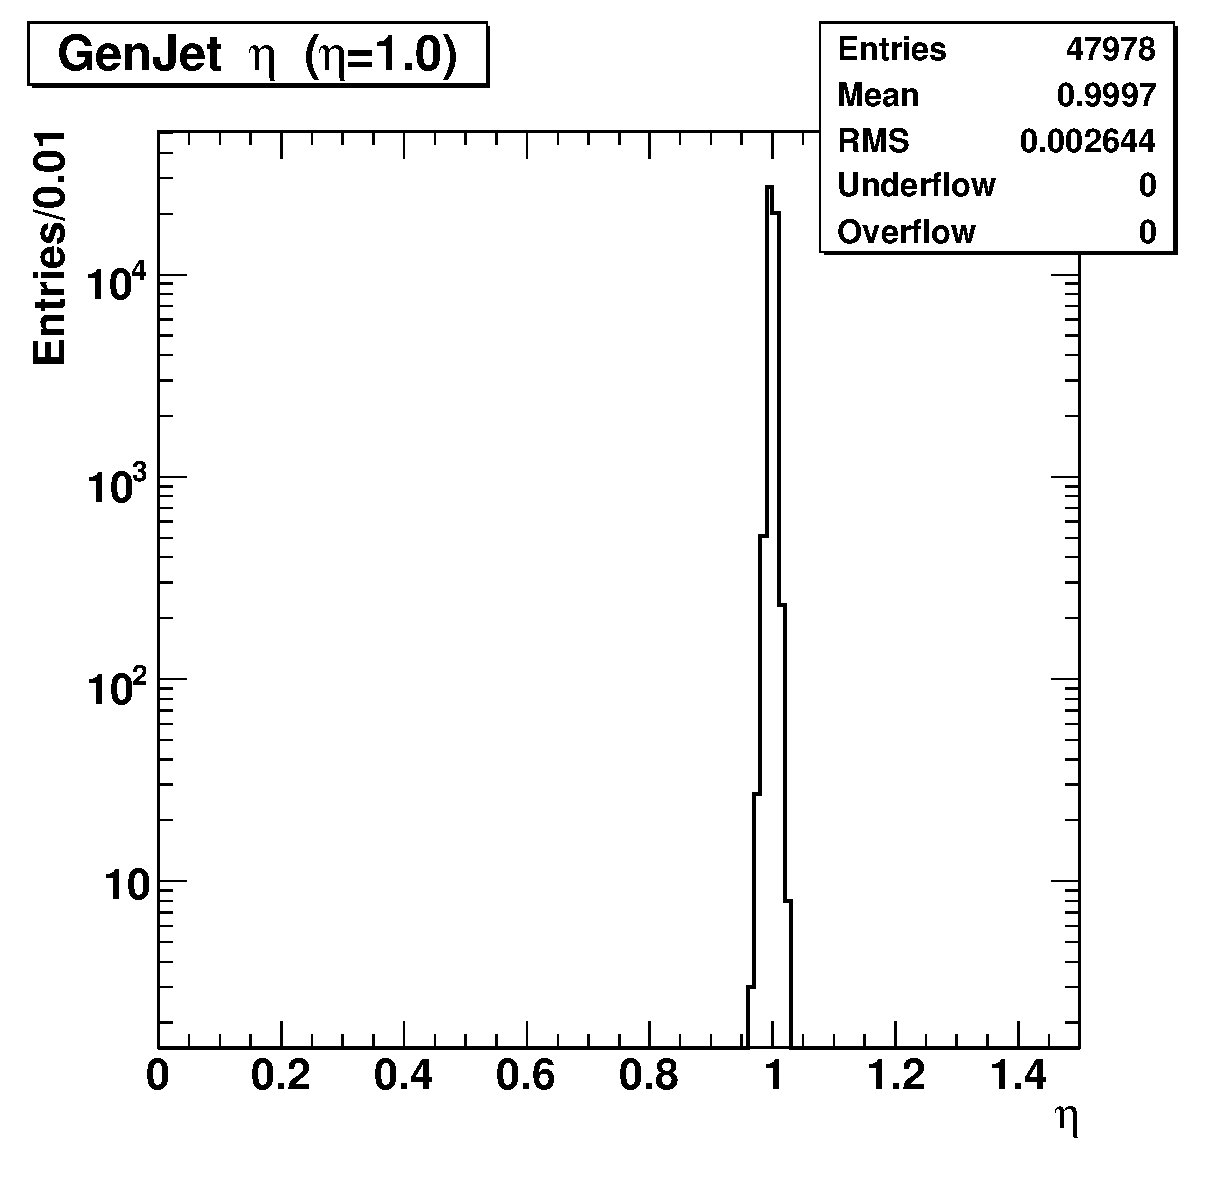
\includegraphics[width=0.31\textwidth]{fig/h_GenJetEta_corr_eta1.0.eps} \\
 \end{tabular}
\end{center}
\begin{center}
 \begin{tabular}{lll}
  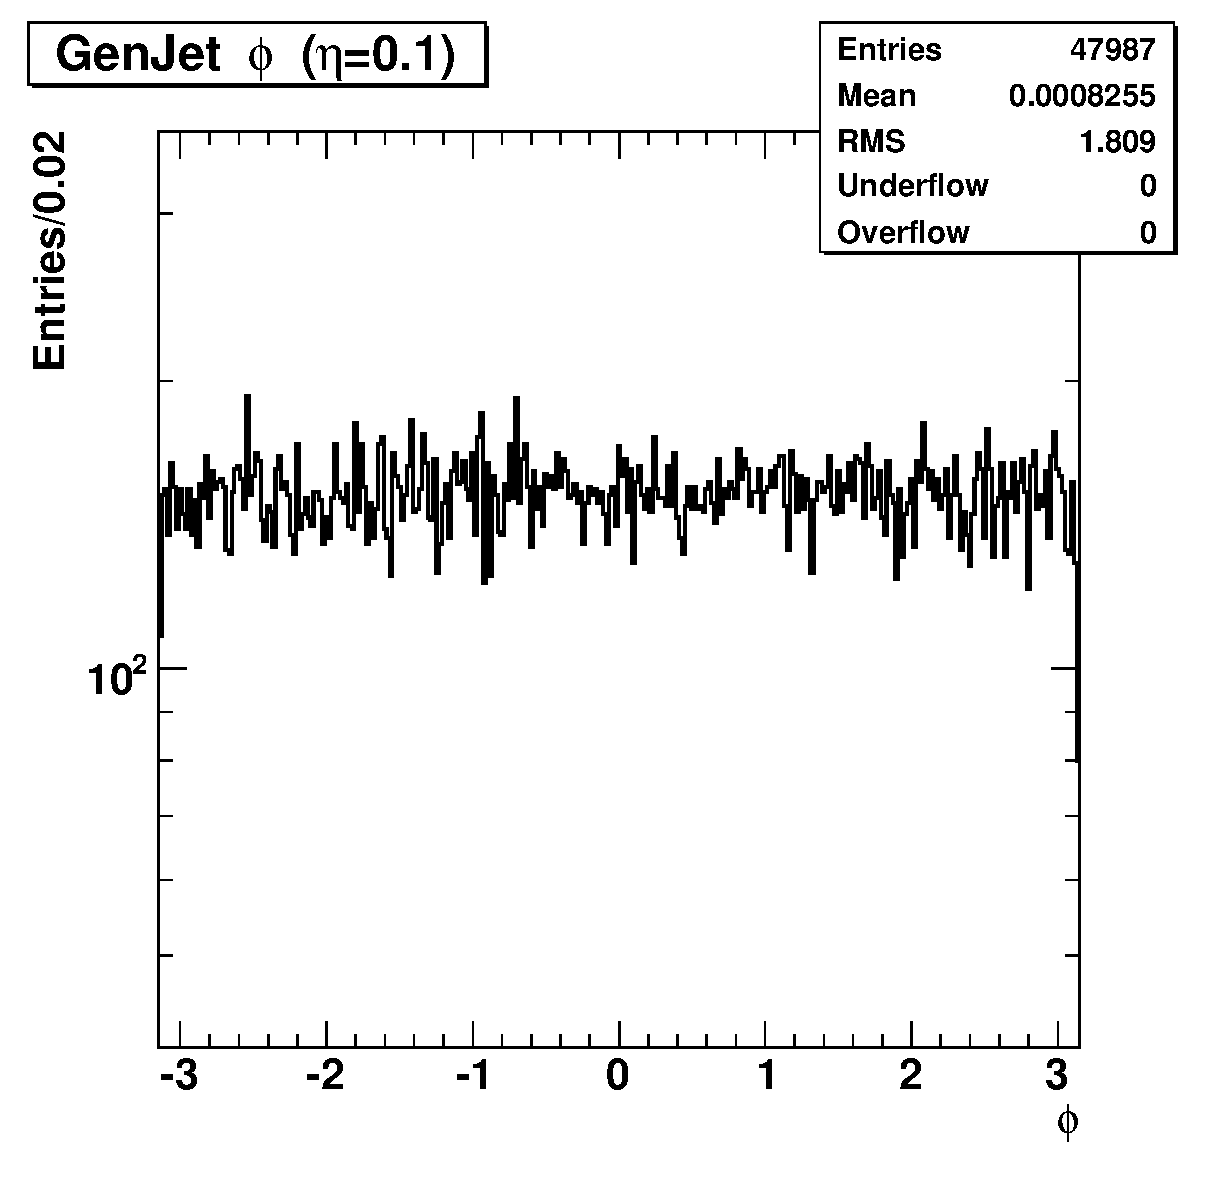
\includegraphics[width=0.31\textwidth]{fig/h_GenJetPhi_corr_eta0.1.eps} &
  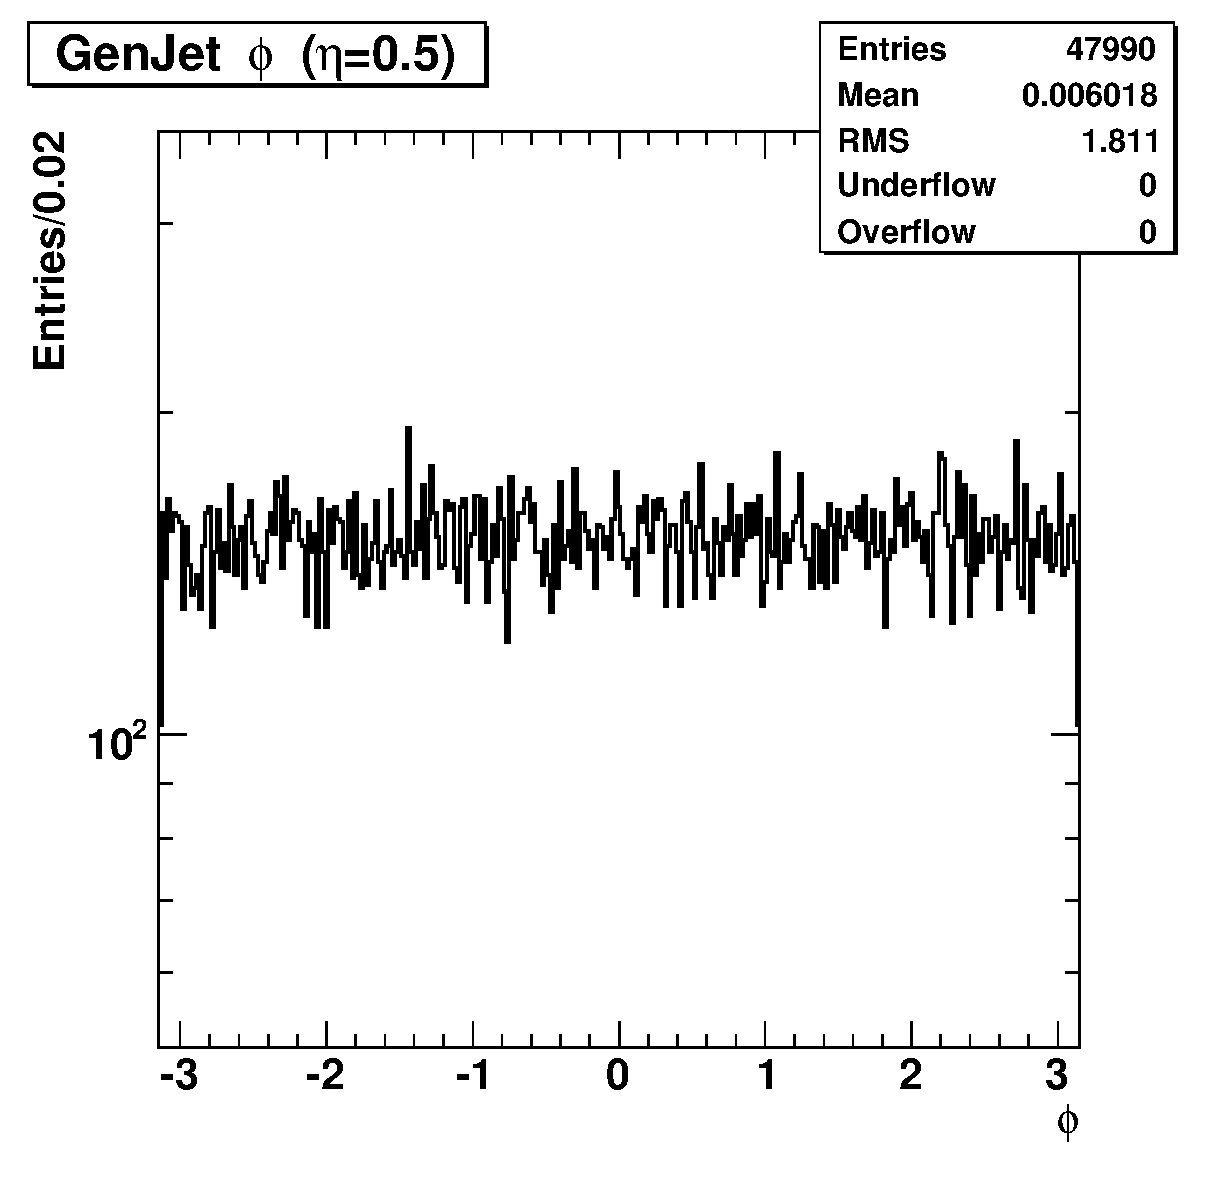
\includegraphics[width=0.31\textwidth]{fig/h_GenJetPhi_corr_eta0.5.eps} &
  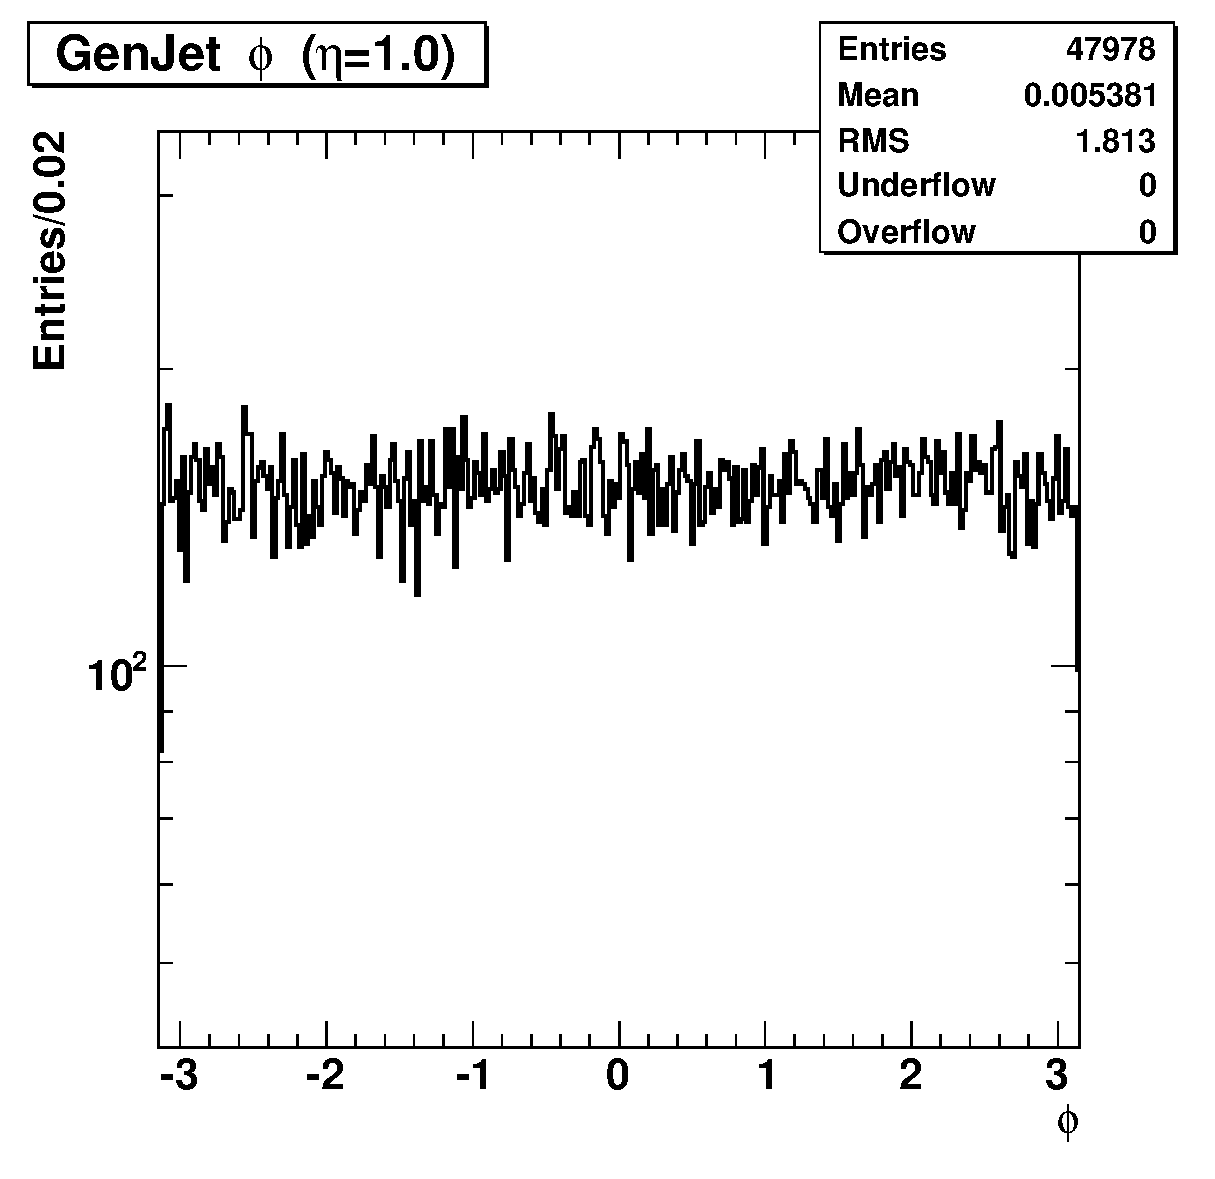
\includegraphics[width=0.31\textwidth]{fig/h_GenJetPhi_corr_eta1.0.eps} \\
 \end{tabular}
\end{center}
\begin{center}
 \begin{tabular}{lll}
  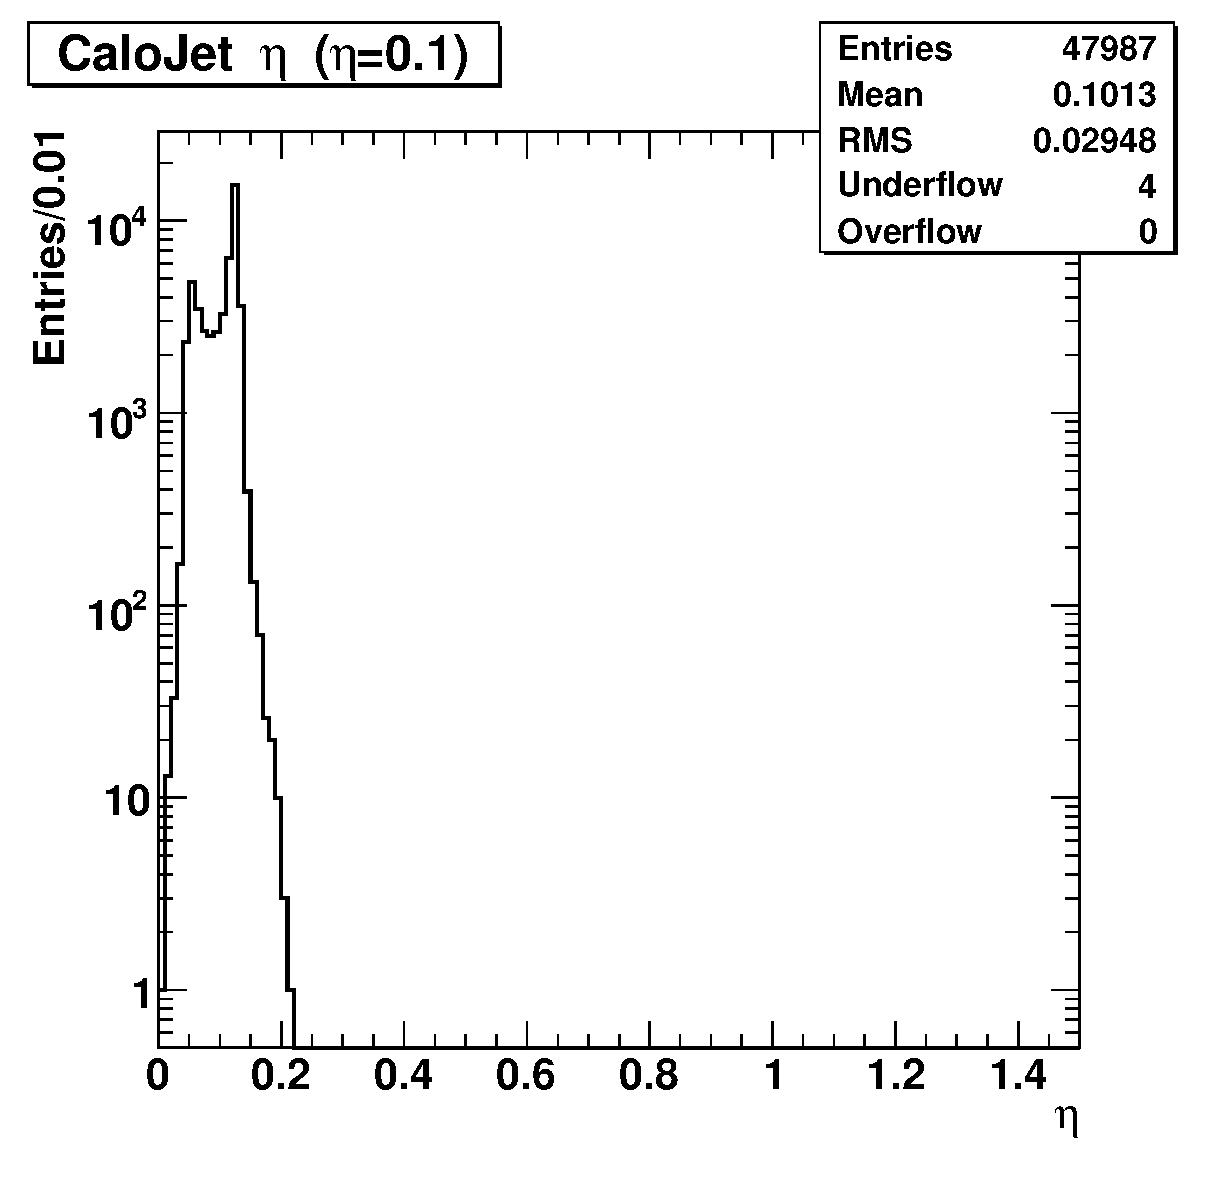
\includegraphics[width=0.31\textwidth]{fig/h_CaloJetEta_corr_eta0.1.eps} &
  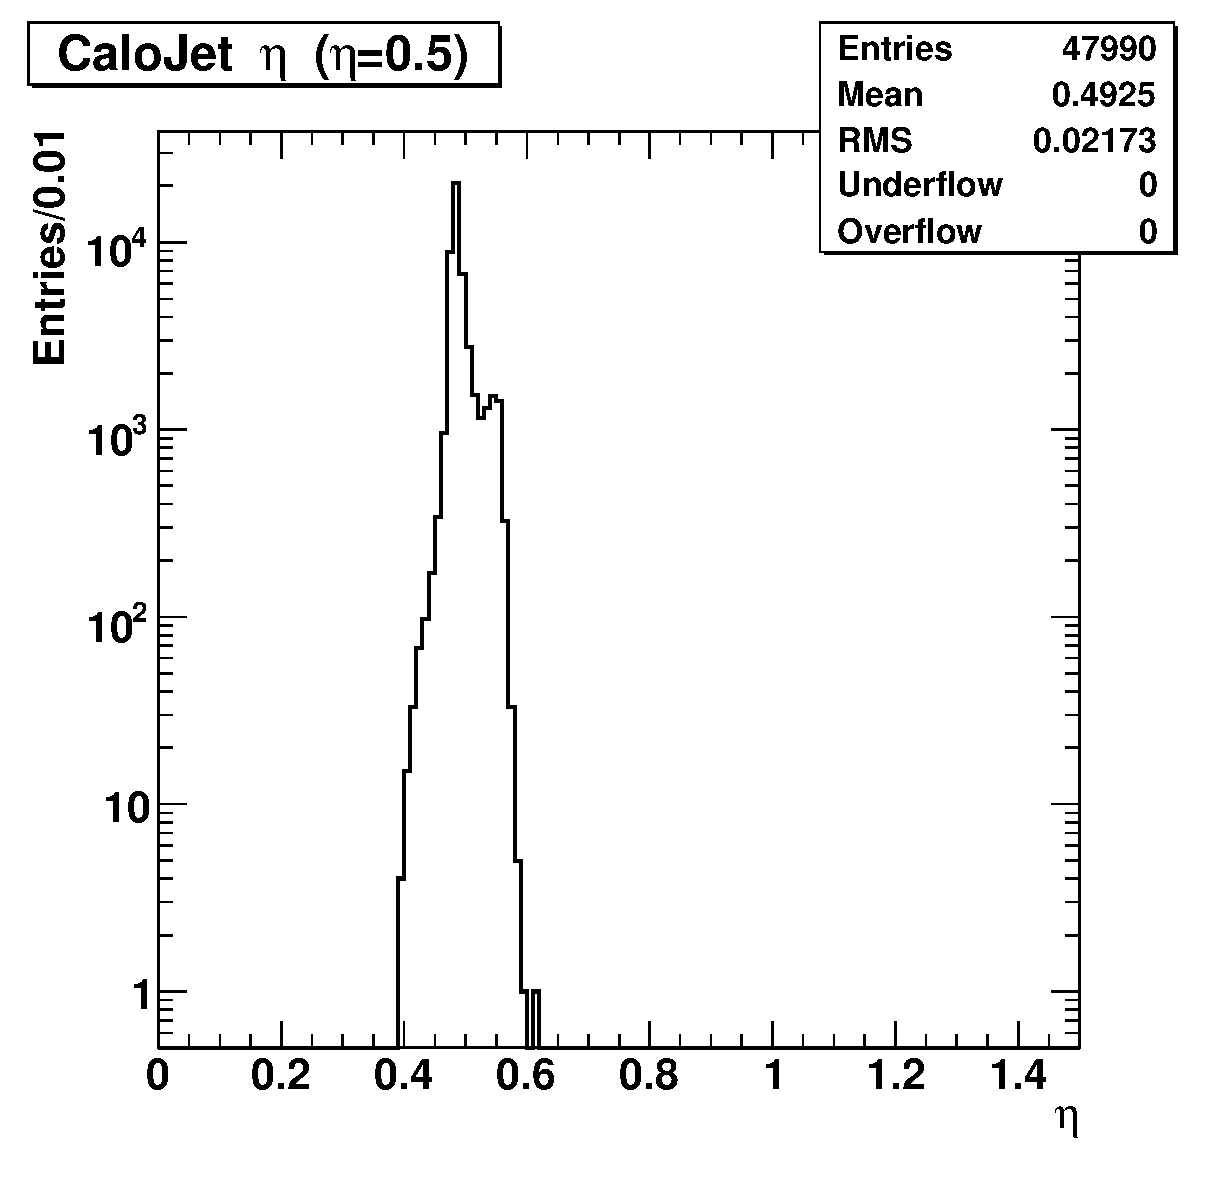
\includegraphics[width=0.31\textwidth]{fig/h_CaloJetEta_corr_eta0.5.eps} &
  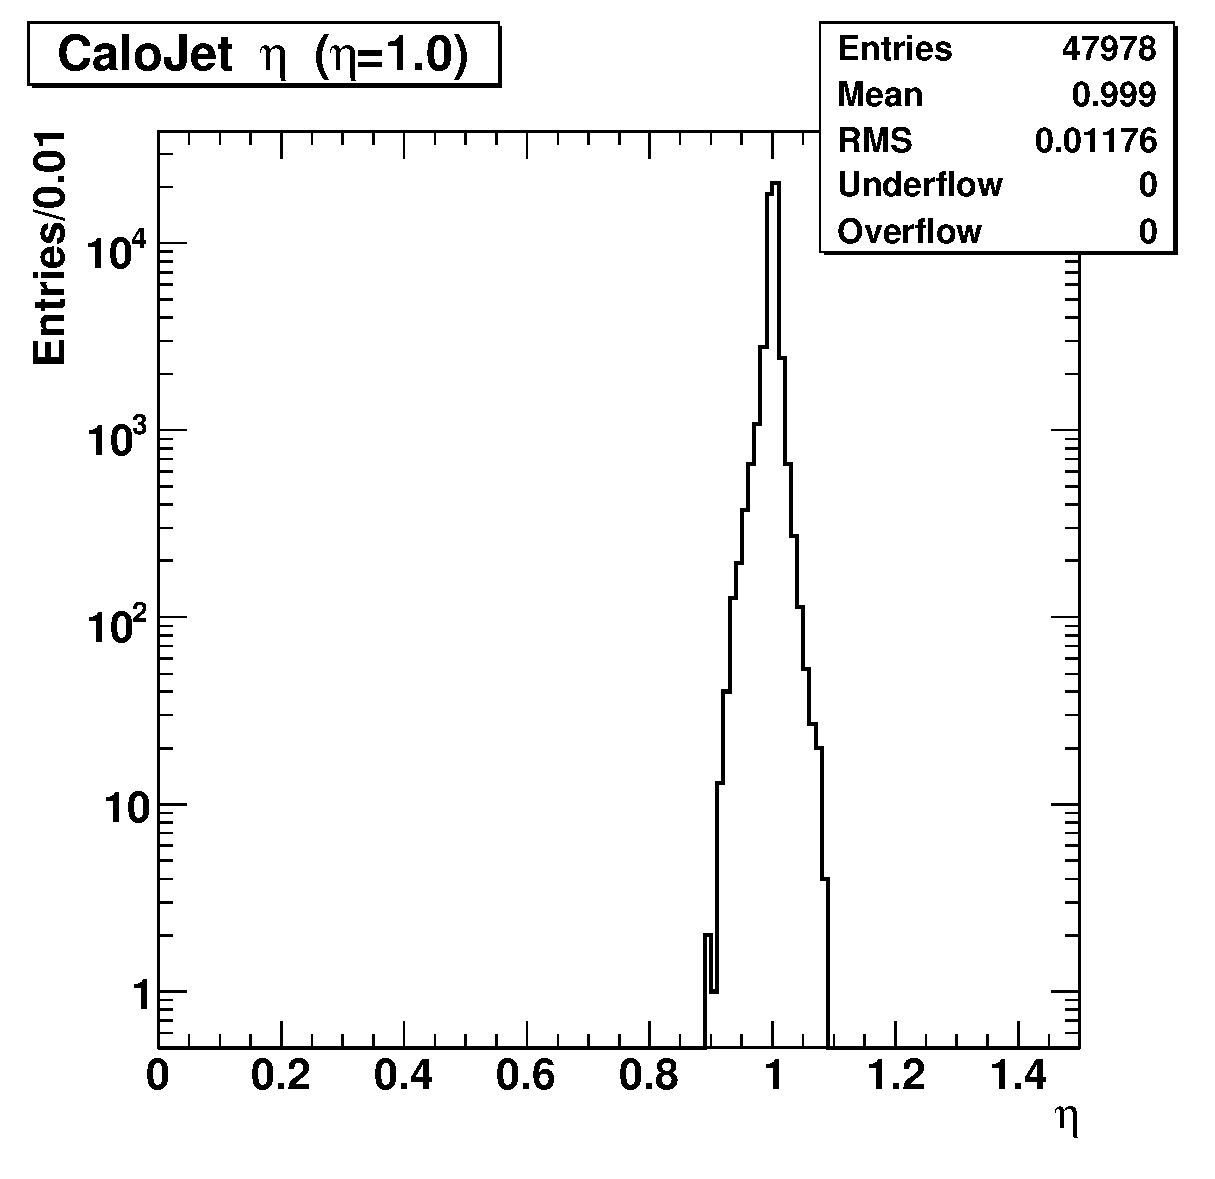
\includegraphics[width=0.31\textwidth]{fig/h_CaloJetEta_corr_eta1.0.eps} \\
 \end{tabular}
\end{center}
\begin{center}
 \begin{tabular}{lll}
  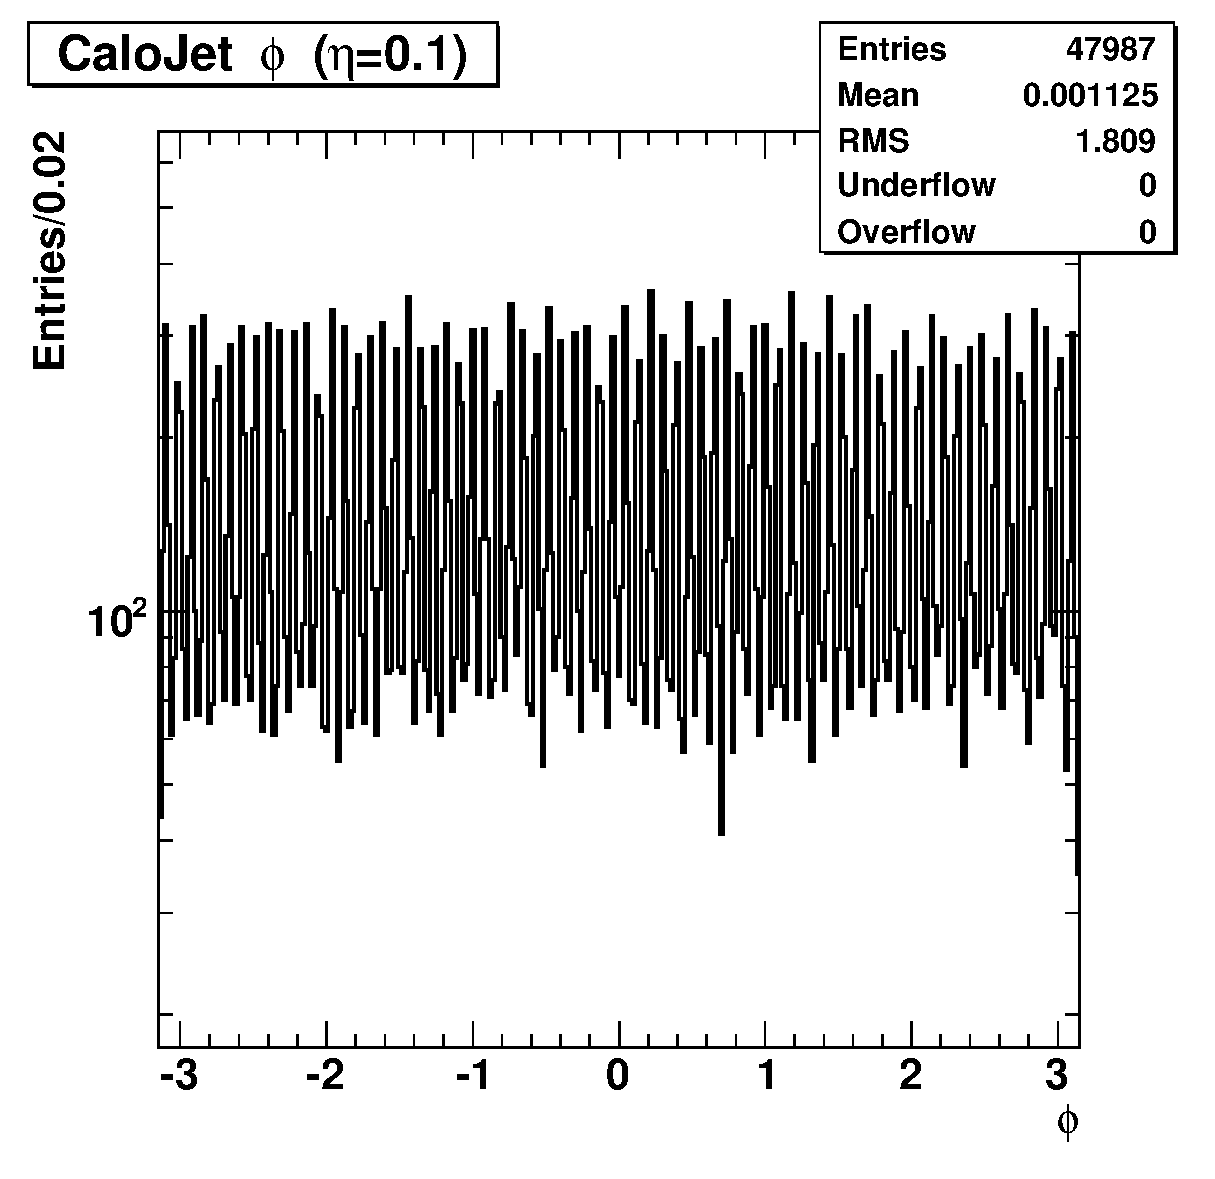
\includegraphics[width=0.31\textwidth]{fig/h_CaloJetPhi_corr_eta0.1.eps} &
  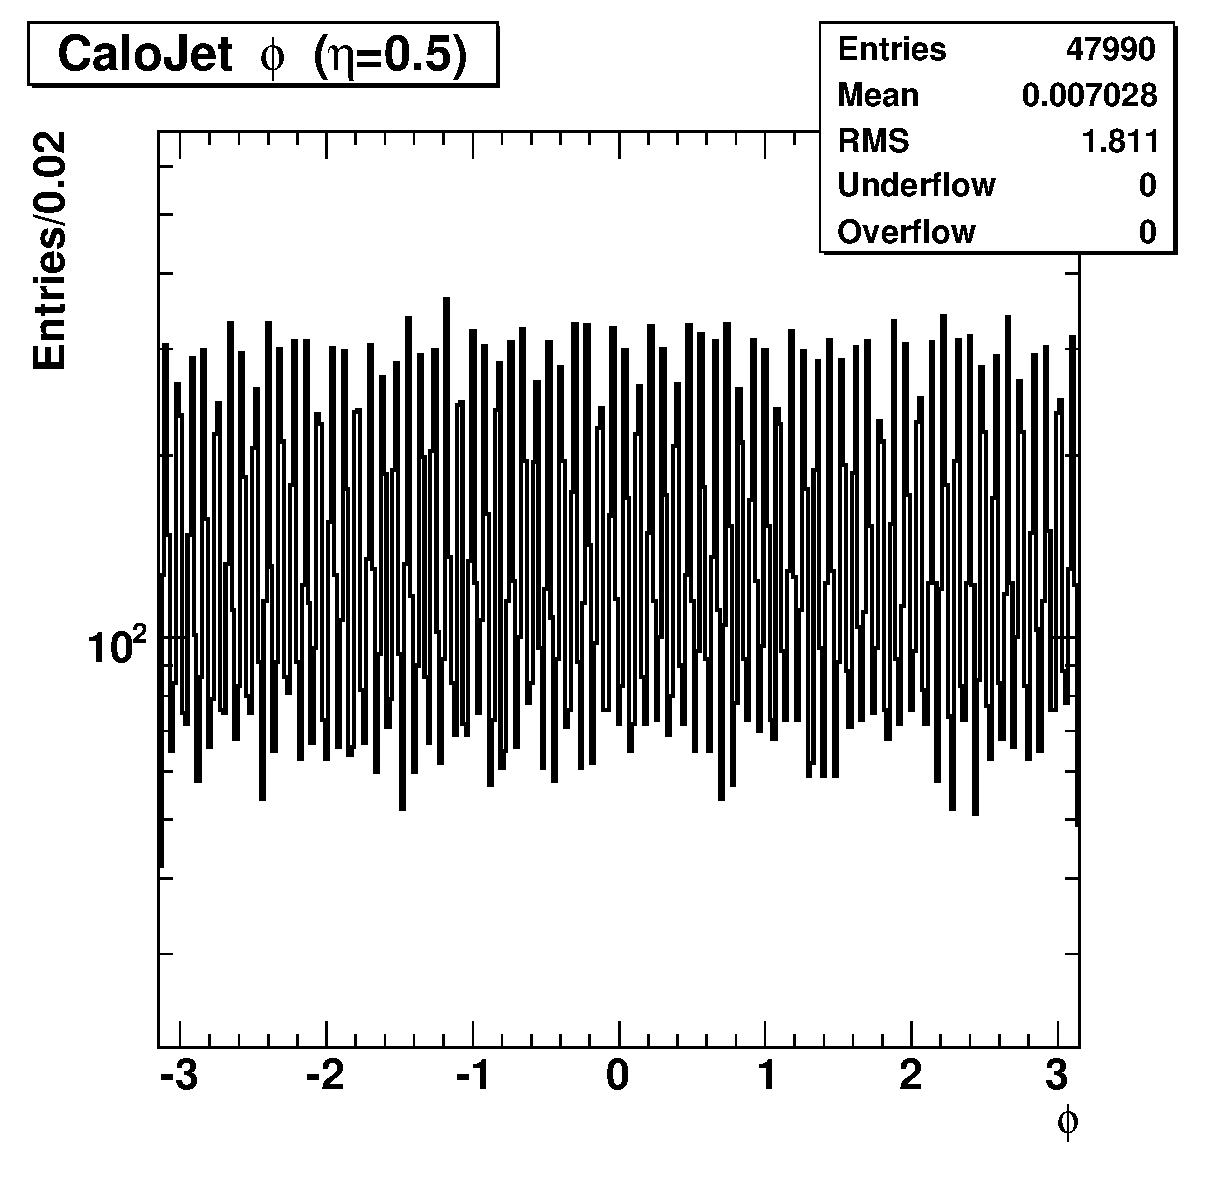
\includegraphics[width=0.31\textwidth]{fig/h_CaloJetPhi_corr_eta0.5.eps} &
  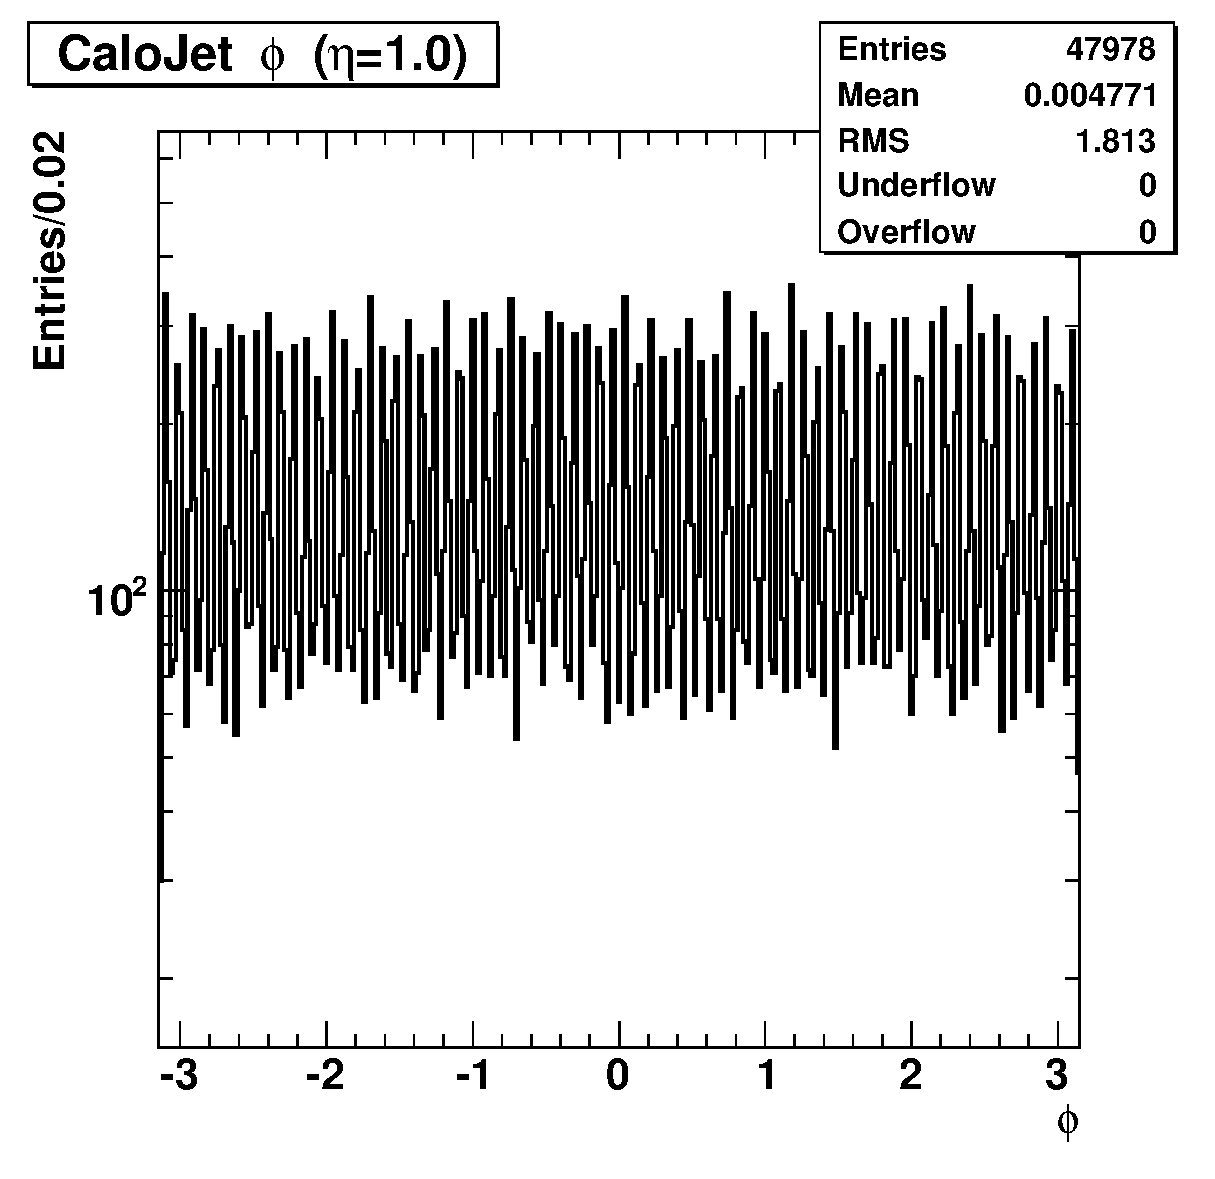
\includegraphics[width=0.31\textwidth]{fig/h_CaloJetPhi_corr_eta1.0.eps} \\
 \end{tabular}
\end{center}
\begin{center}
 \begin{tabular}{lll}
  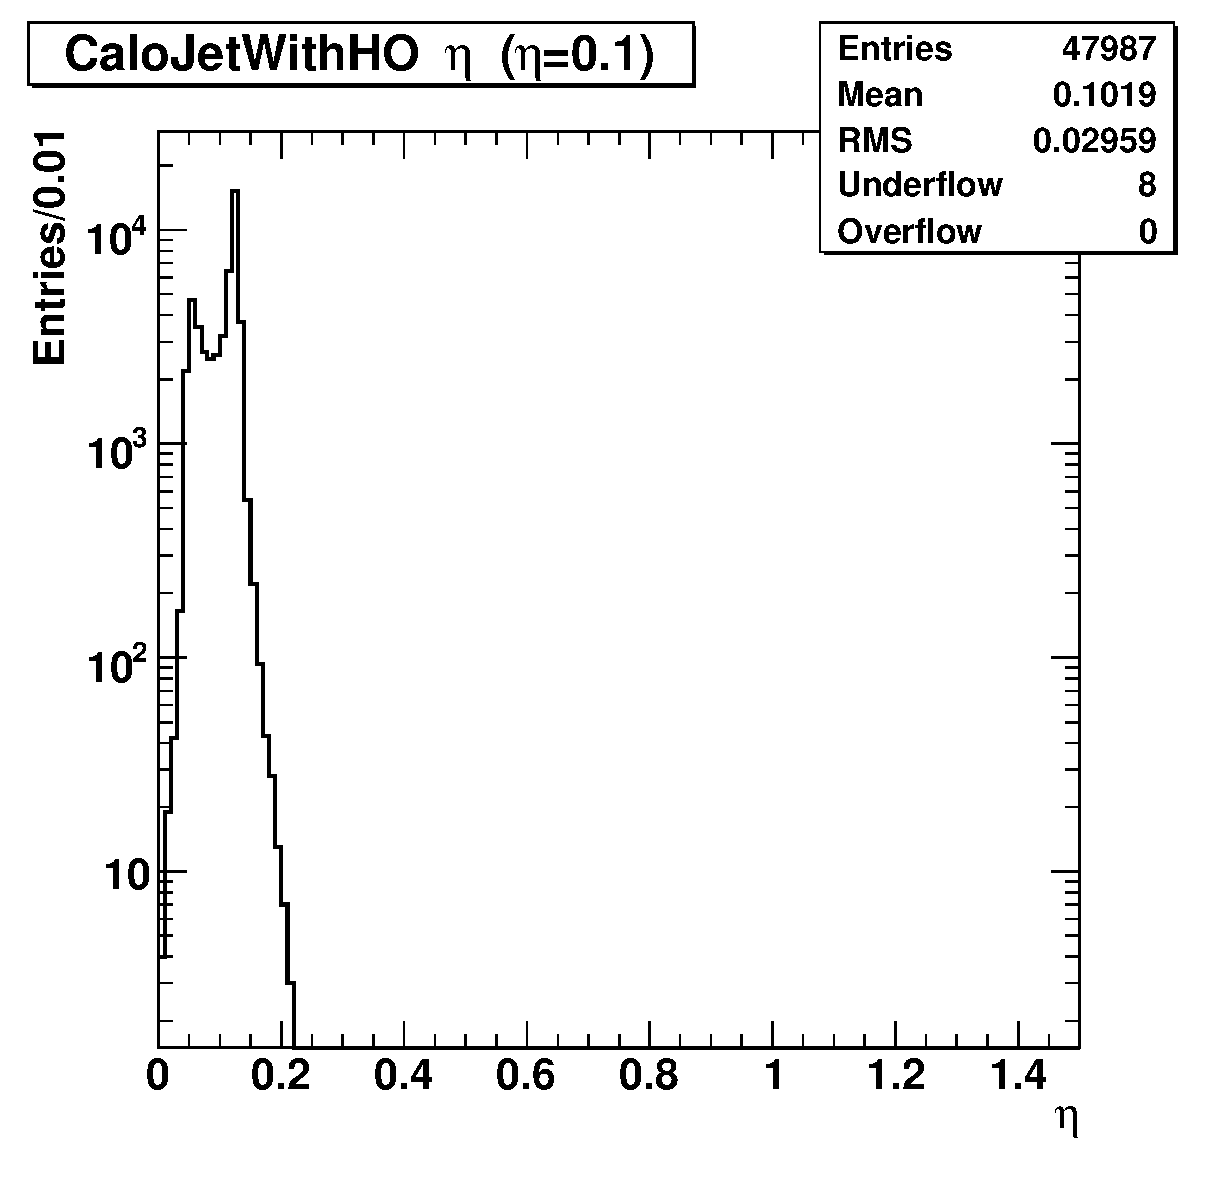
\includegraphics[width=0.31\textwidth]{fig/h_CaloJetWithHOEta_corr_eta0.1.eps} &
  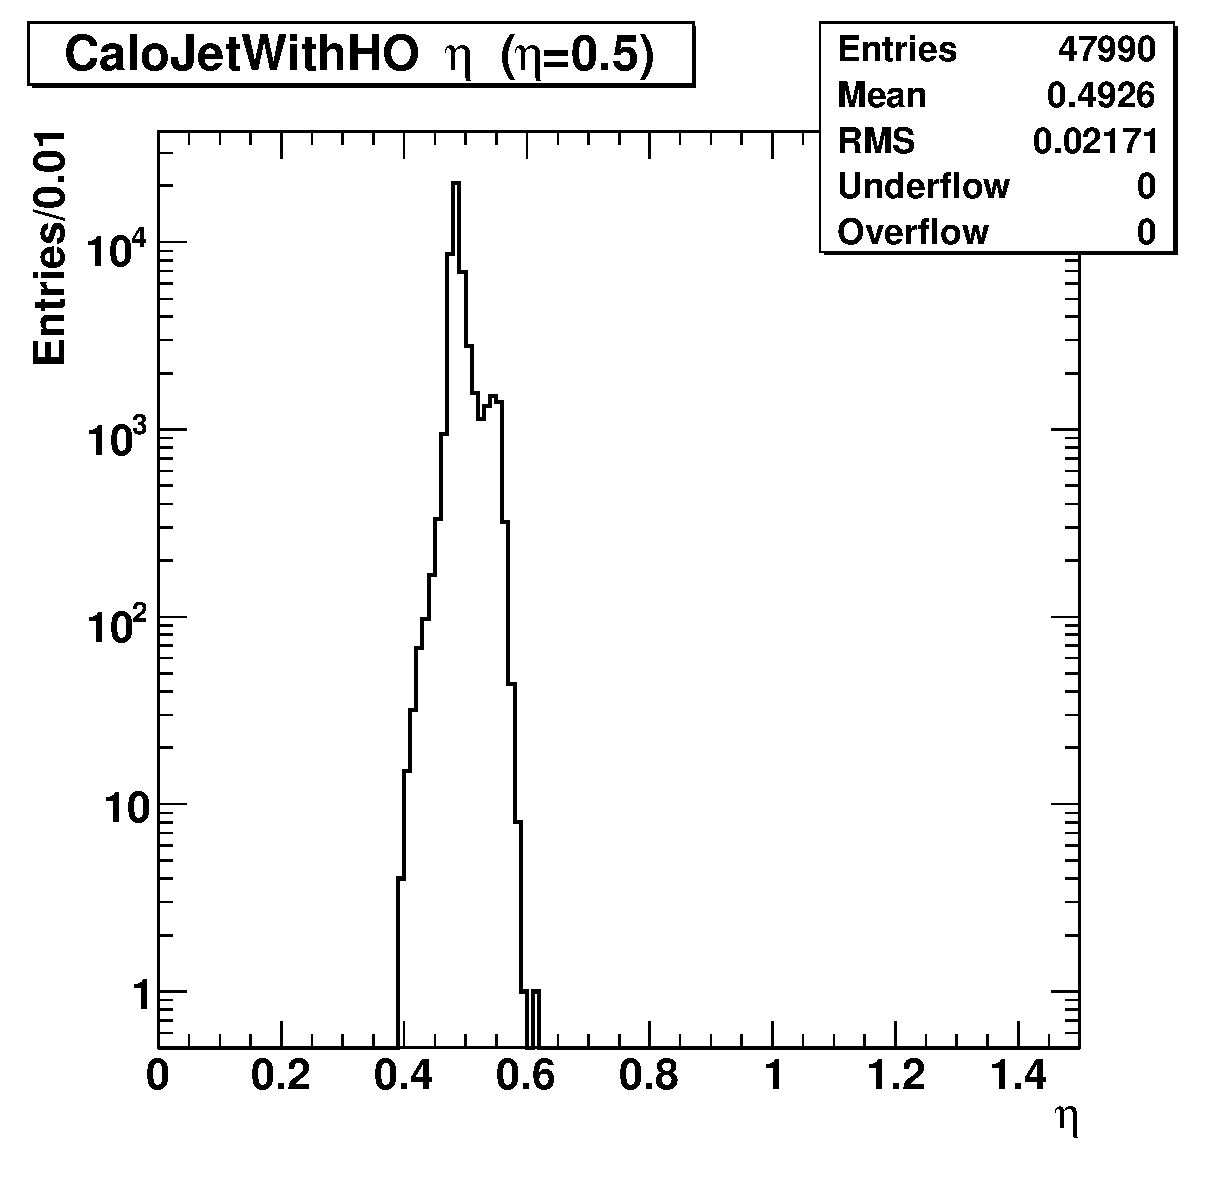
\includegraphics[width=0.31\textwidth]{fig/h_CaloJetWithHOEta_corr_eta0.5.eps} &
  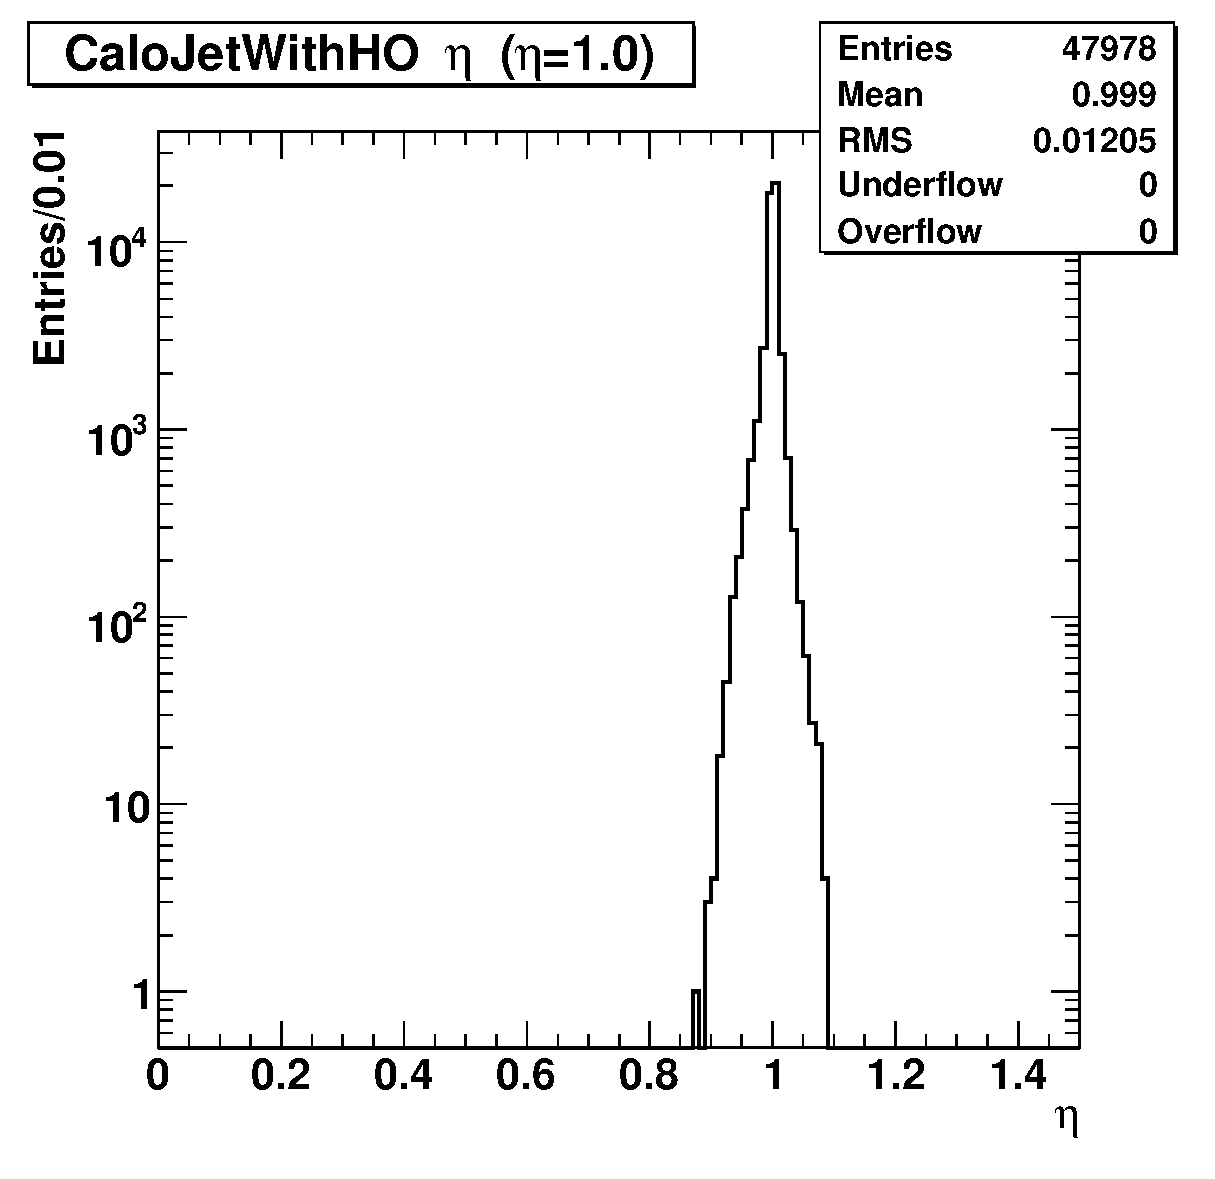
\includegraphics[width=0.31\textwidth]{fig/h_CaloJetWithHOEta_corr_eta1.0.eps} \\
 \end{tabular}
\end{center}
\begin{center}
 \begin{tabular}{lll}
  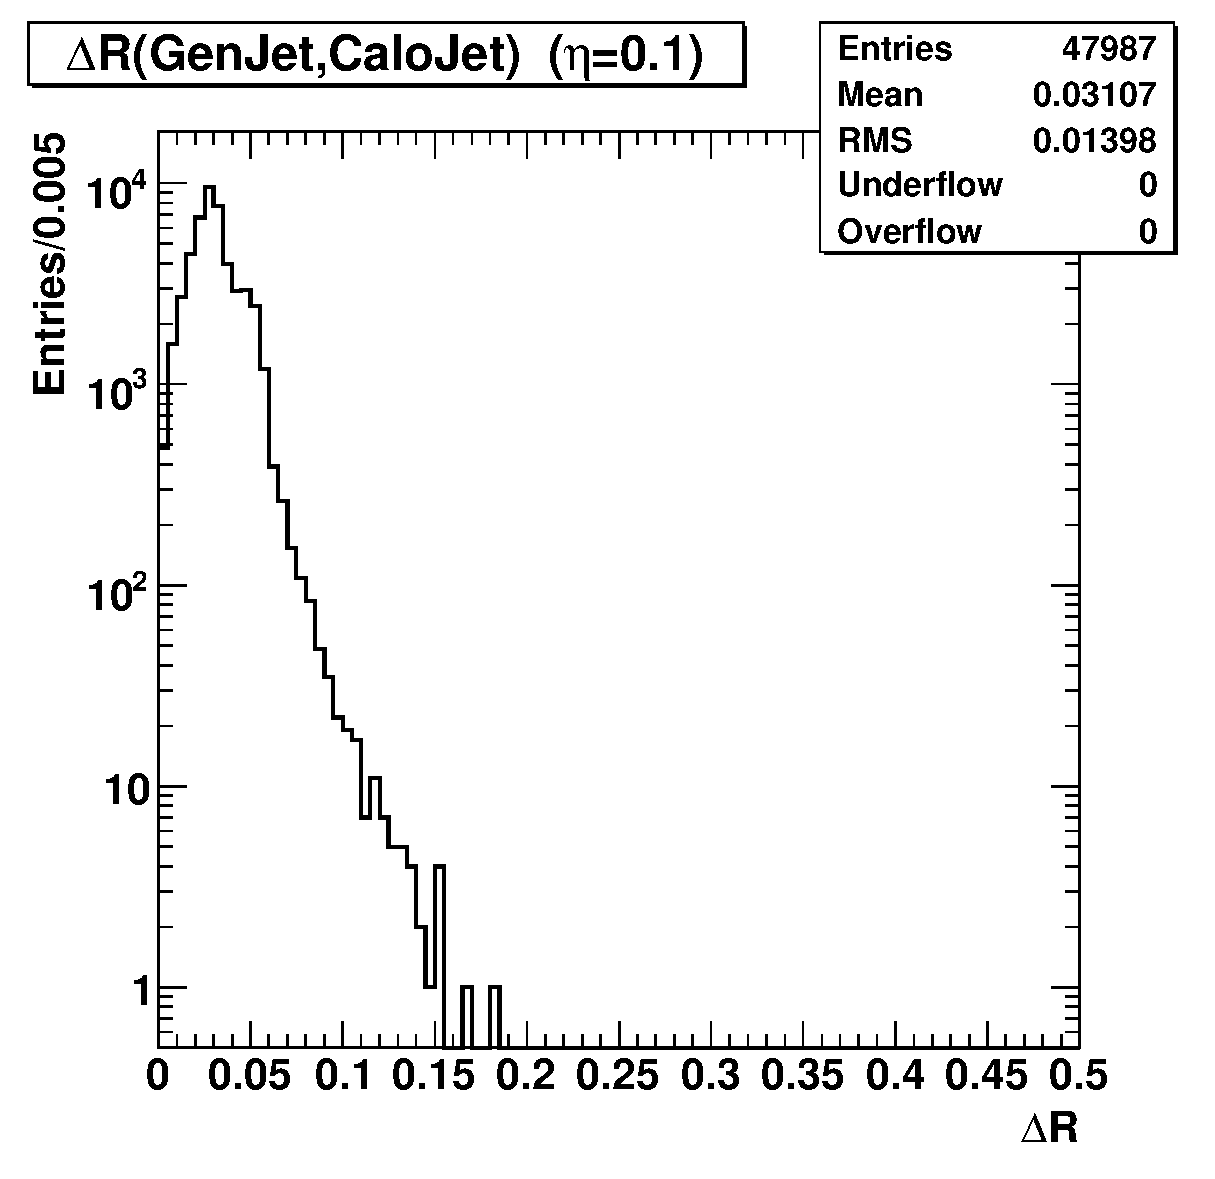
\includegraphics[width=0.31\textwidth]{fig/h_DeltaR_corr_eta0.1.eps} &
  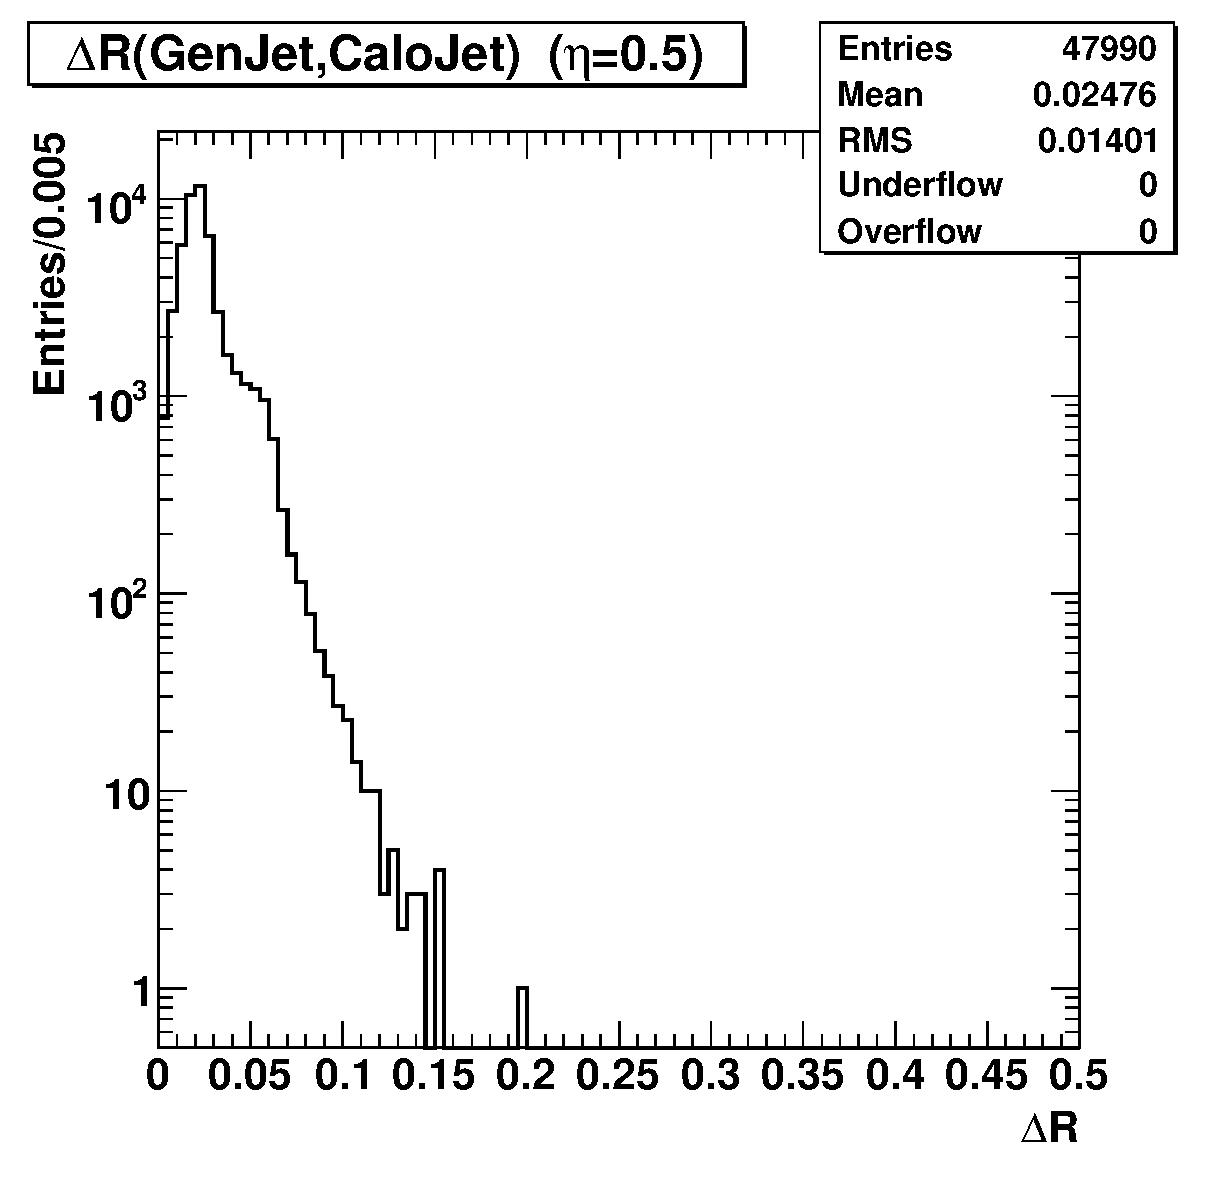
\includegraphics[width=0.31\textwidth]{fig/h_DeltaR_corr_eta0.5.eps} &
  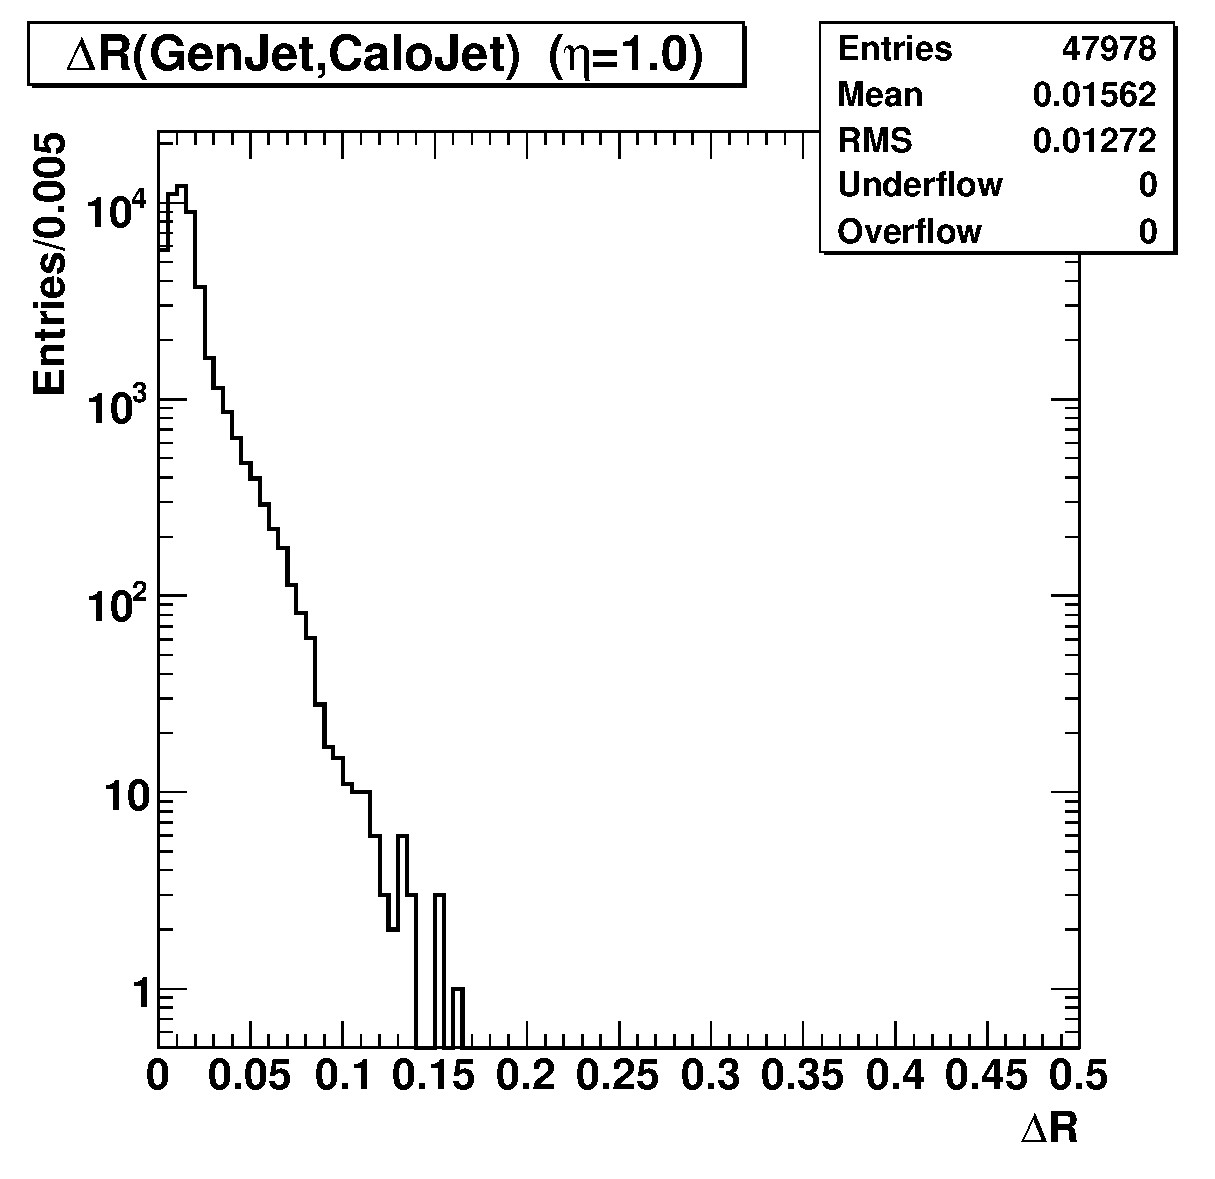
\includegraphics[width=0.31\textwidth]{fig/h_DeltaR_corr_eta1.0.eps} \\
 \end{tabular}
\end{center}
\begin{center}
 \begin{tabular}{lll}
  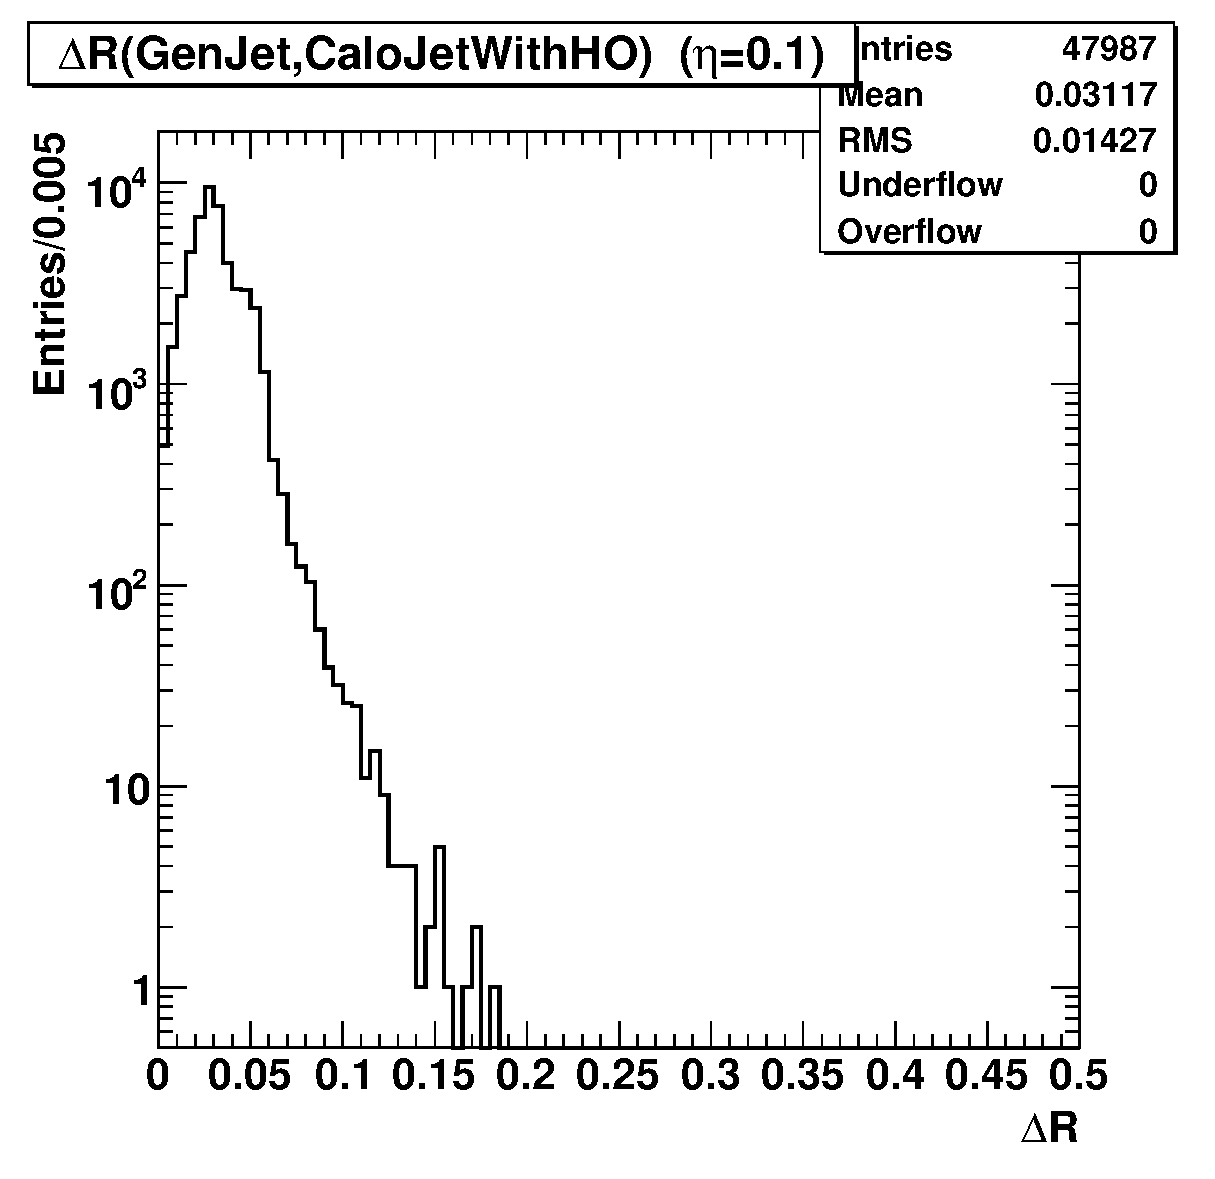
\includegraphics[width=0.31\textwidth]{fig/h_DeltaRWithHO_corr_eta0.1.eps} &
  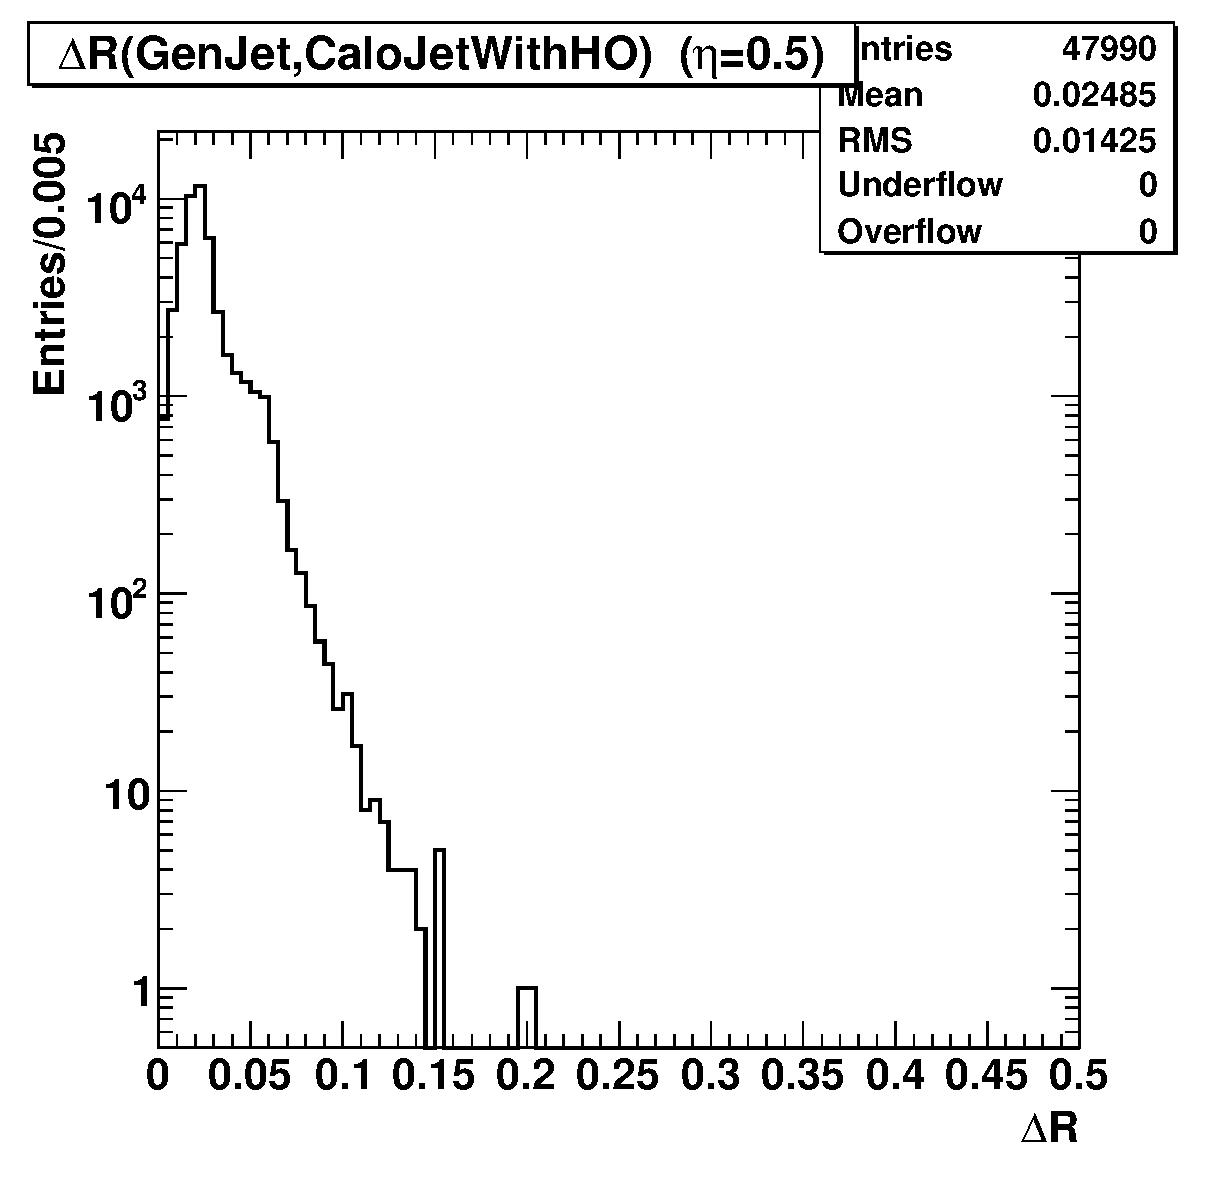
\includegraphics[width=0.31\textwidth]{fig/h_DeltaRWithHO_corr_eta0.5.eps} &
  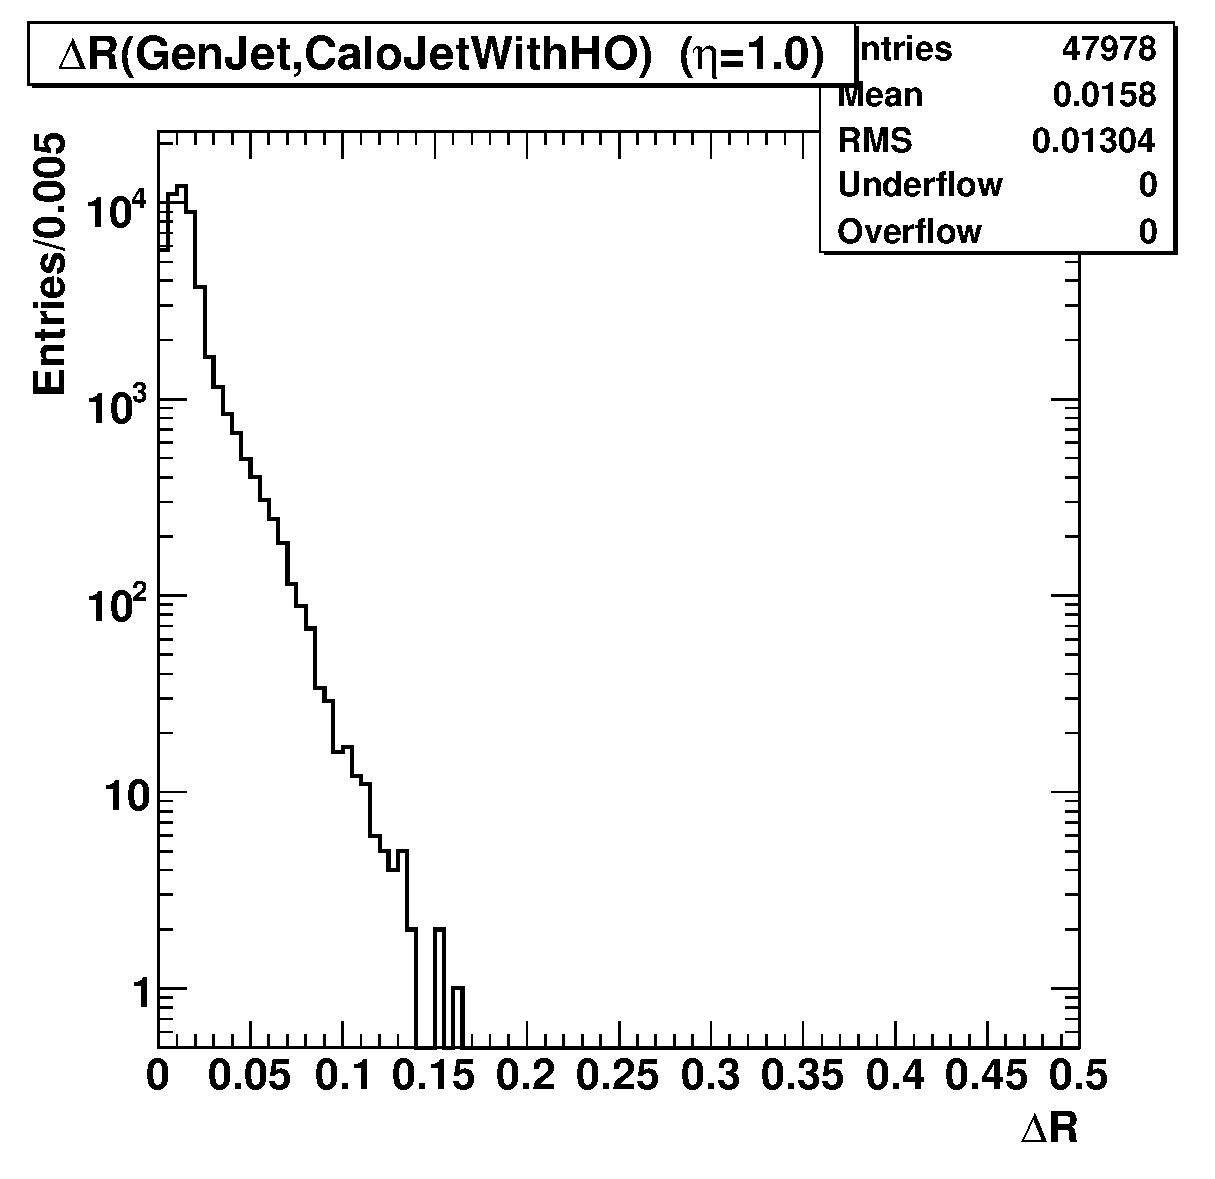
\includegraphics[width=0.31\textwidth]{fig/h_DeltaRWithHO_corr_eta1.0.eps} \\
 \end{tabular}
\end{center}


\section{$\bp_\mathrm{T}$ Spectra of the GenJet Constituent Particles}
\label{app:pT_spect}

\begin{center}
\begin{tabular}{lll}
 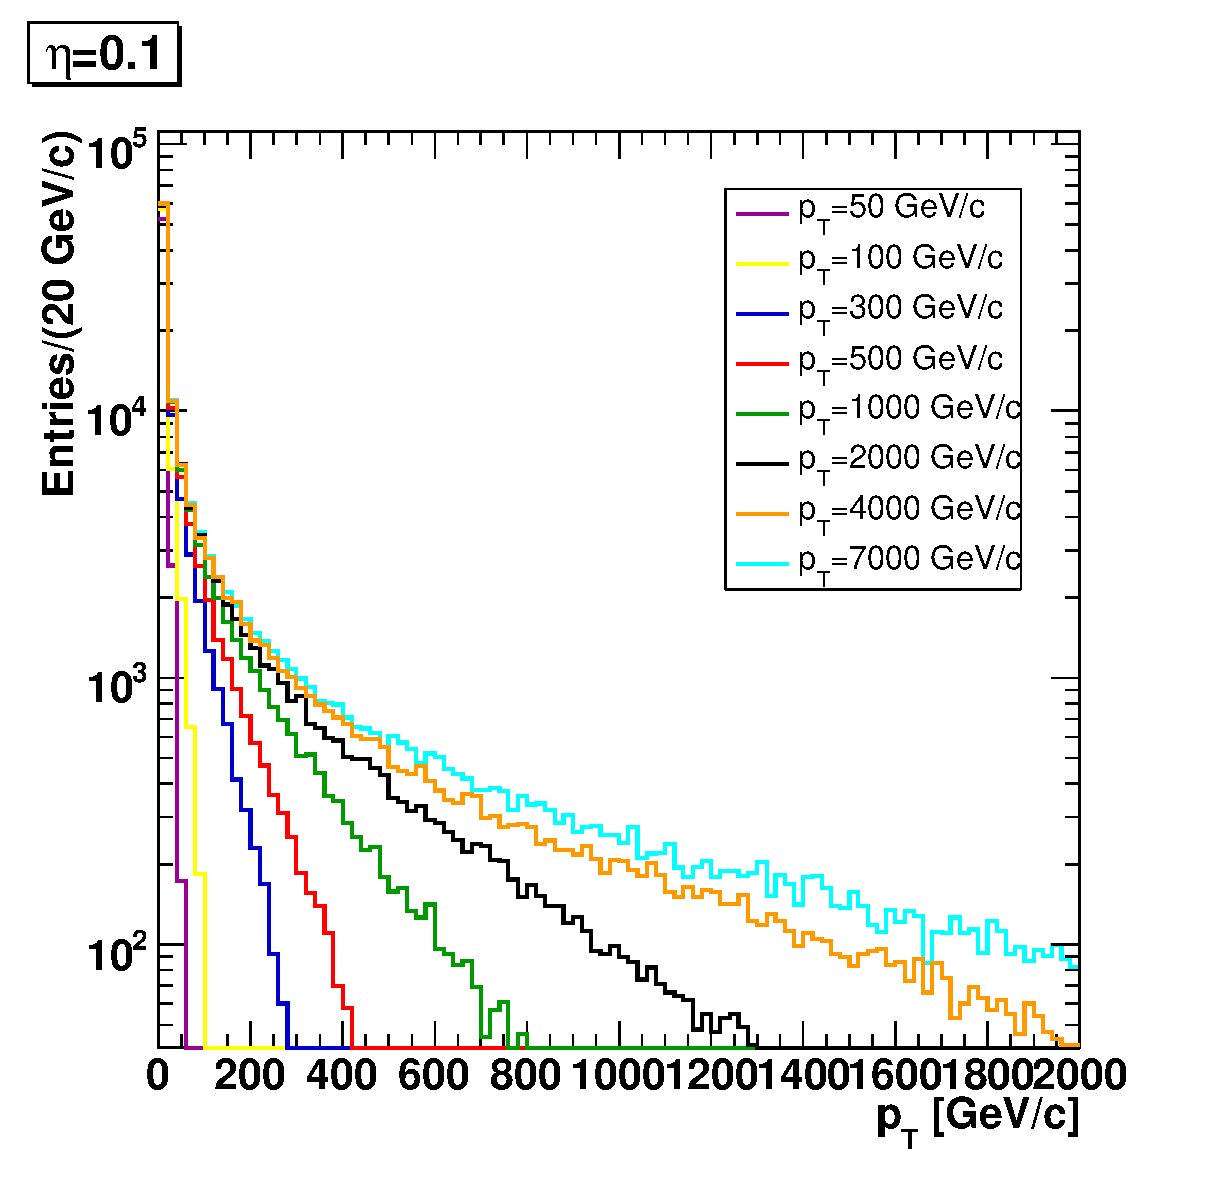
\includegraphics[width=0.31\textwidth]{fig/h_ConstituentpT_ET_py_corr_eta0.1.eps} &
 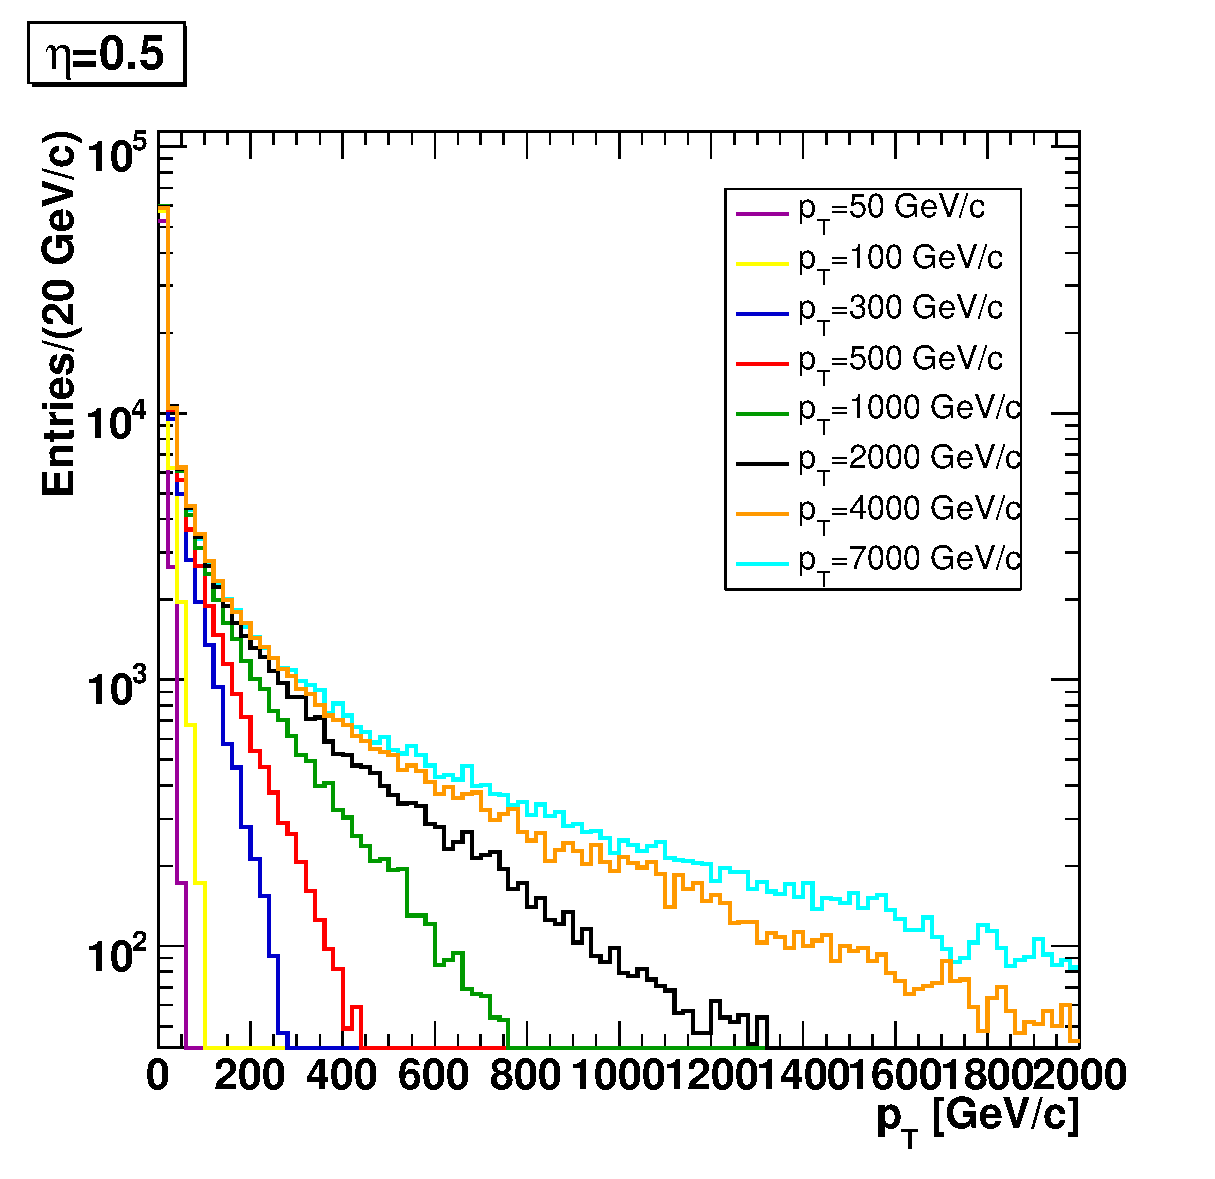
\includegraphics[width=0.31\textwidth]{fig/h_ConstituentpT_ET_py_corr_eta0.5.eps} &
 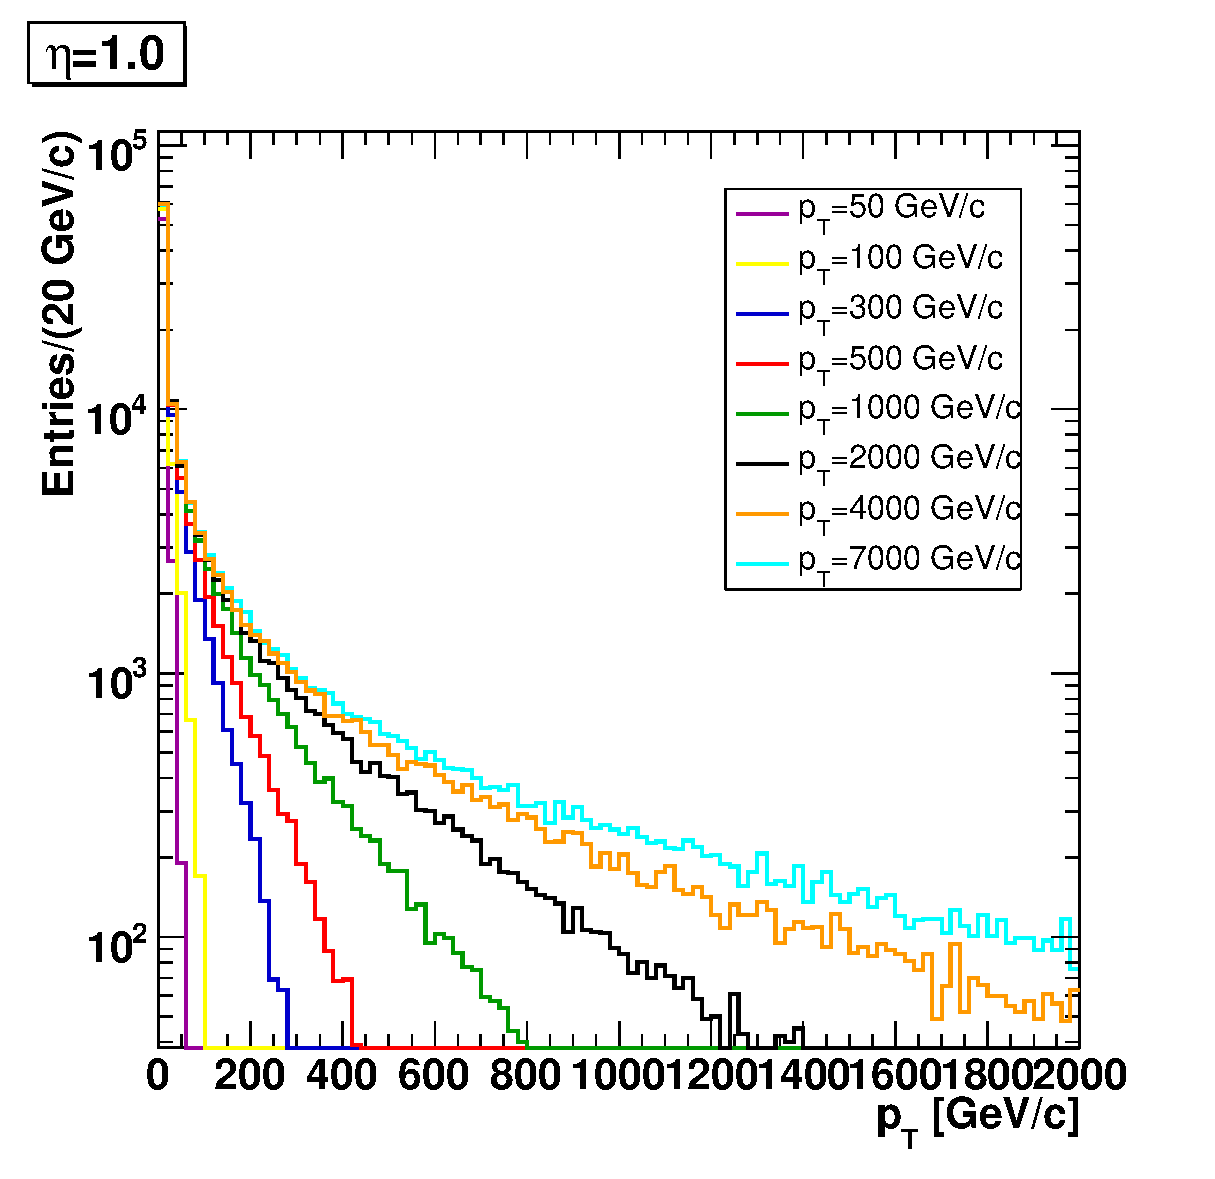
\includegraphics[width=0.31\textwidth]{fig/h_ConstituentpT_ET_py_corr_eta1.0.eps} \\
\end{tabular}
\end{center}
\begin{center}
\begin{tabular}{lll}
 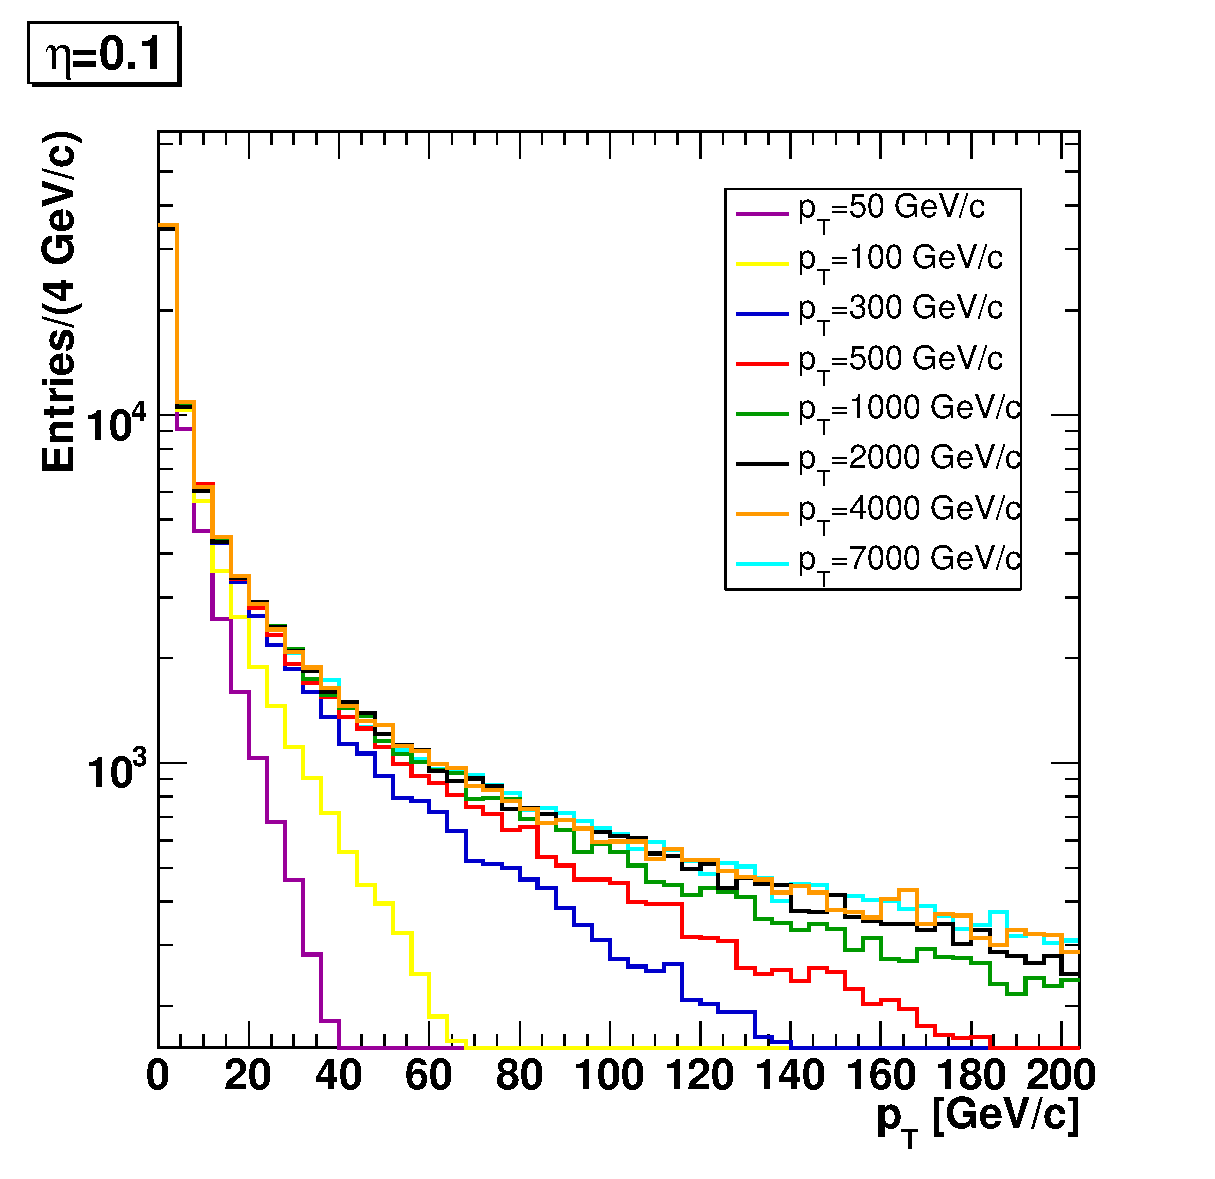
\includegraphics[width=0.31\textwidth]{fig/h_ConstituentpT_ET_py_corr_eta0.1_zoomed.eps} &
 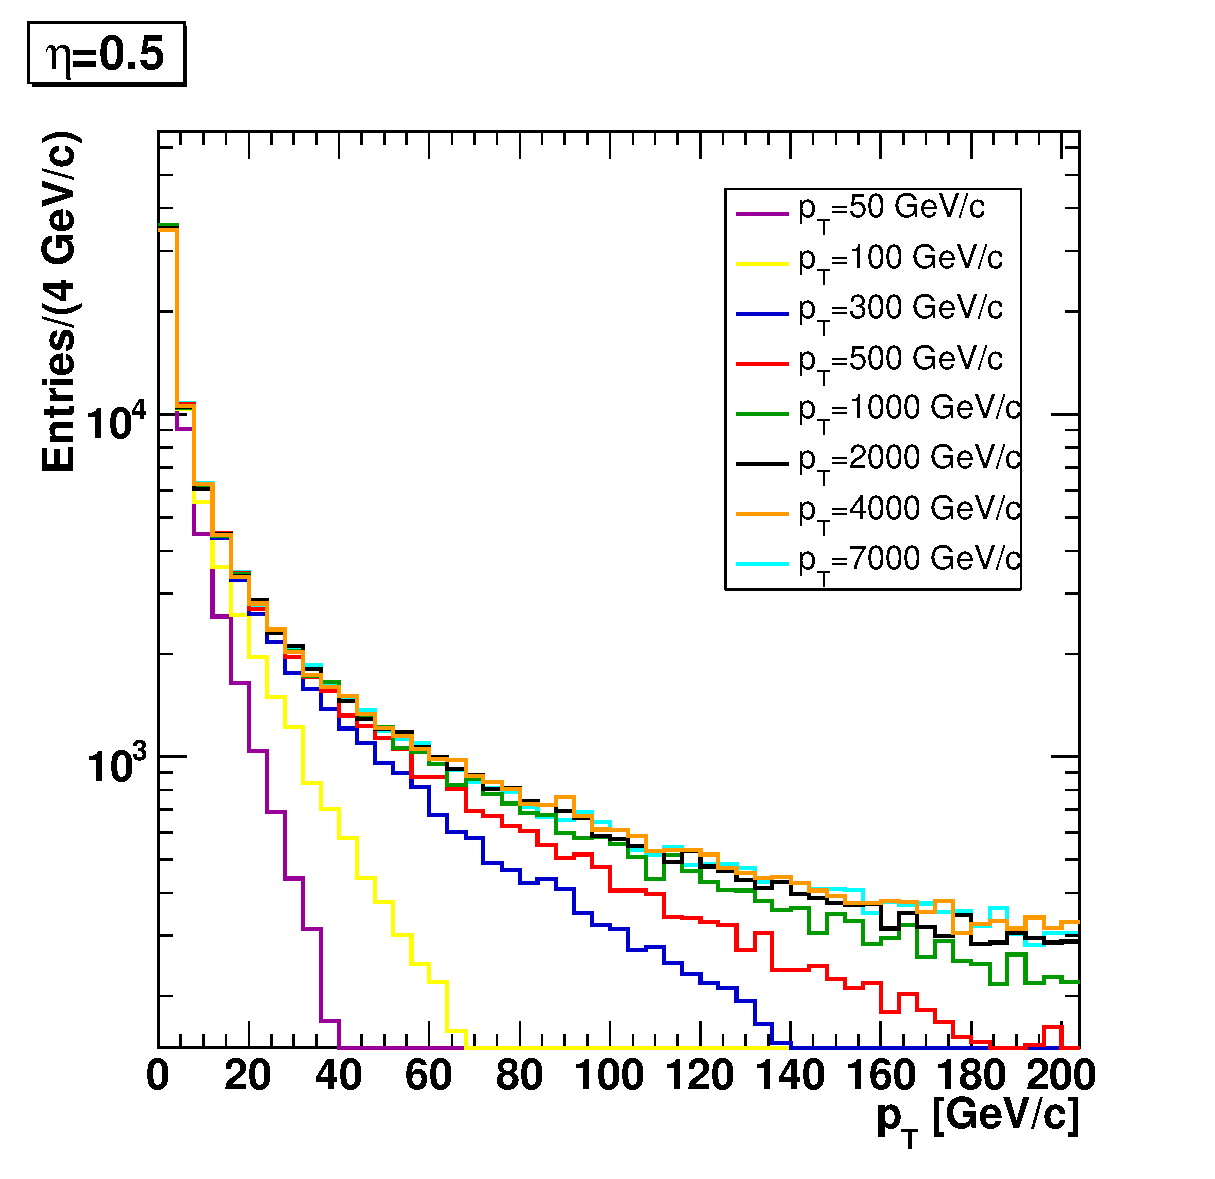
\includegraphics[width=0.31\textwidth]{fig/h_ConstituentpT_ET_py_corr_eta0.5_zoomed.eps} &
 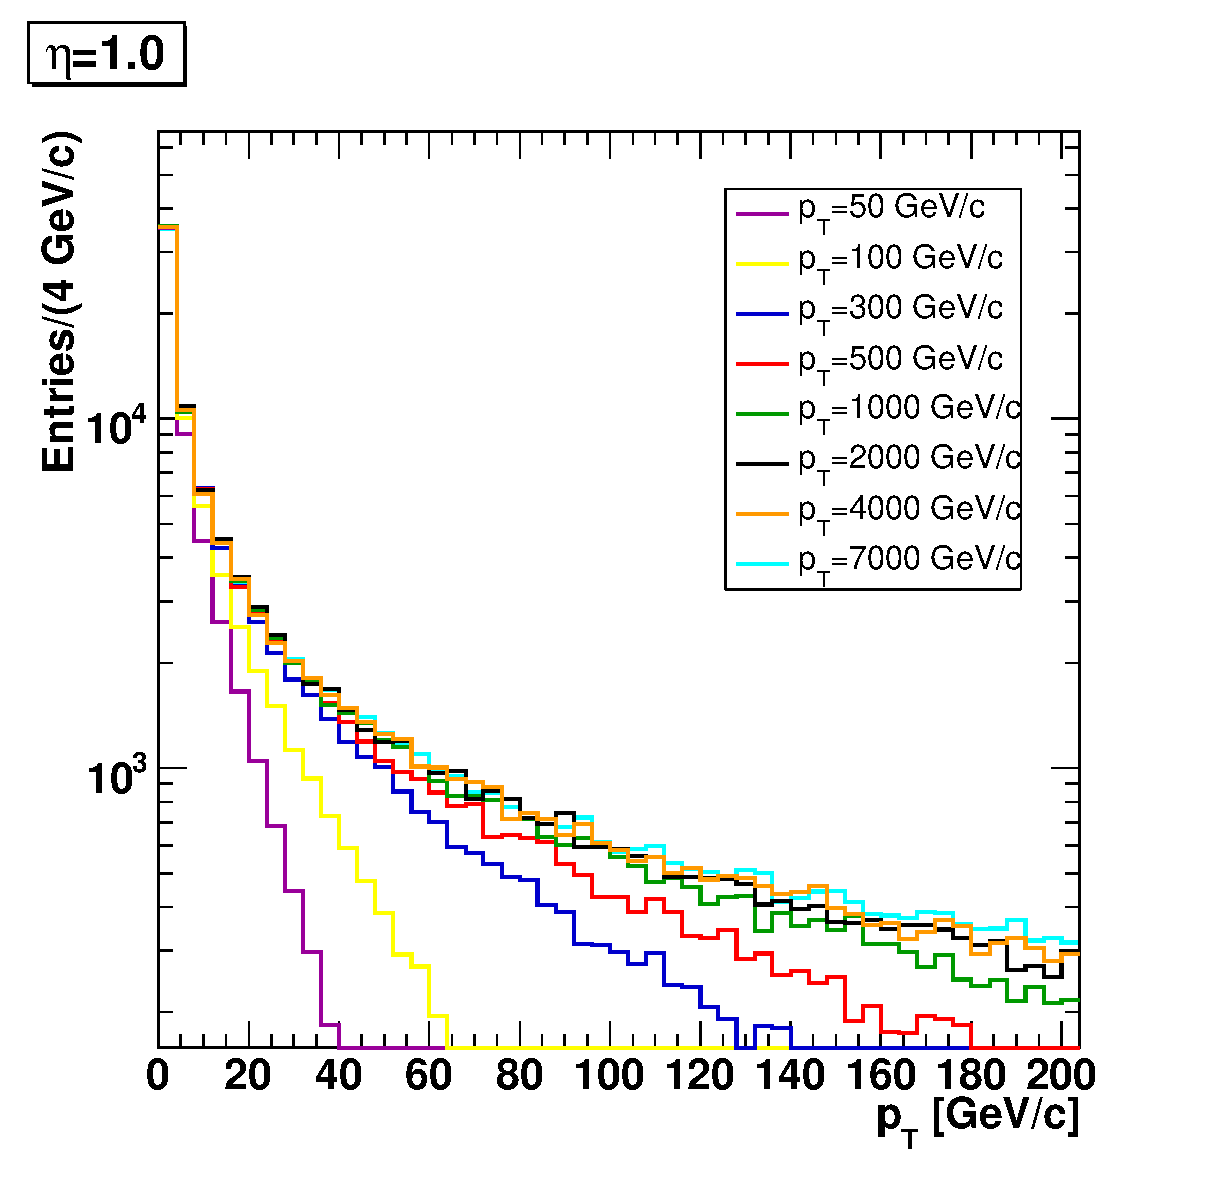
\includegraphics[width=0.31\textwidth]{fig/h_ConstituentpT_ET_py_corr_eta1.0_zoomed.eps} \\
\end{tabular}
\end{center}

\section{Gaussian Fits}
\label{app:fits}

\subsection{CaloJets}

\begin{center}
\begin{tabular}{lll}
 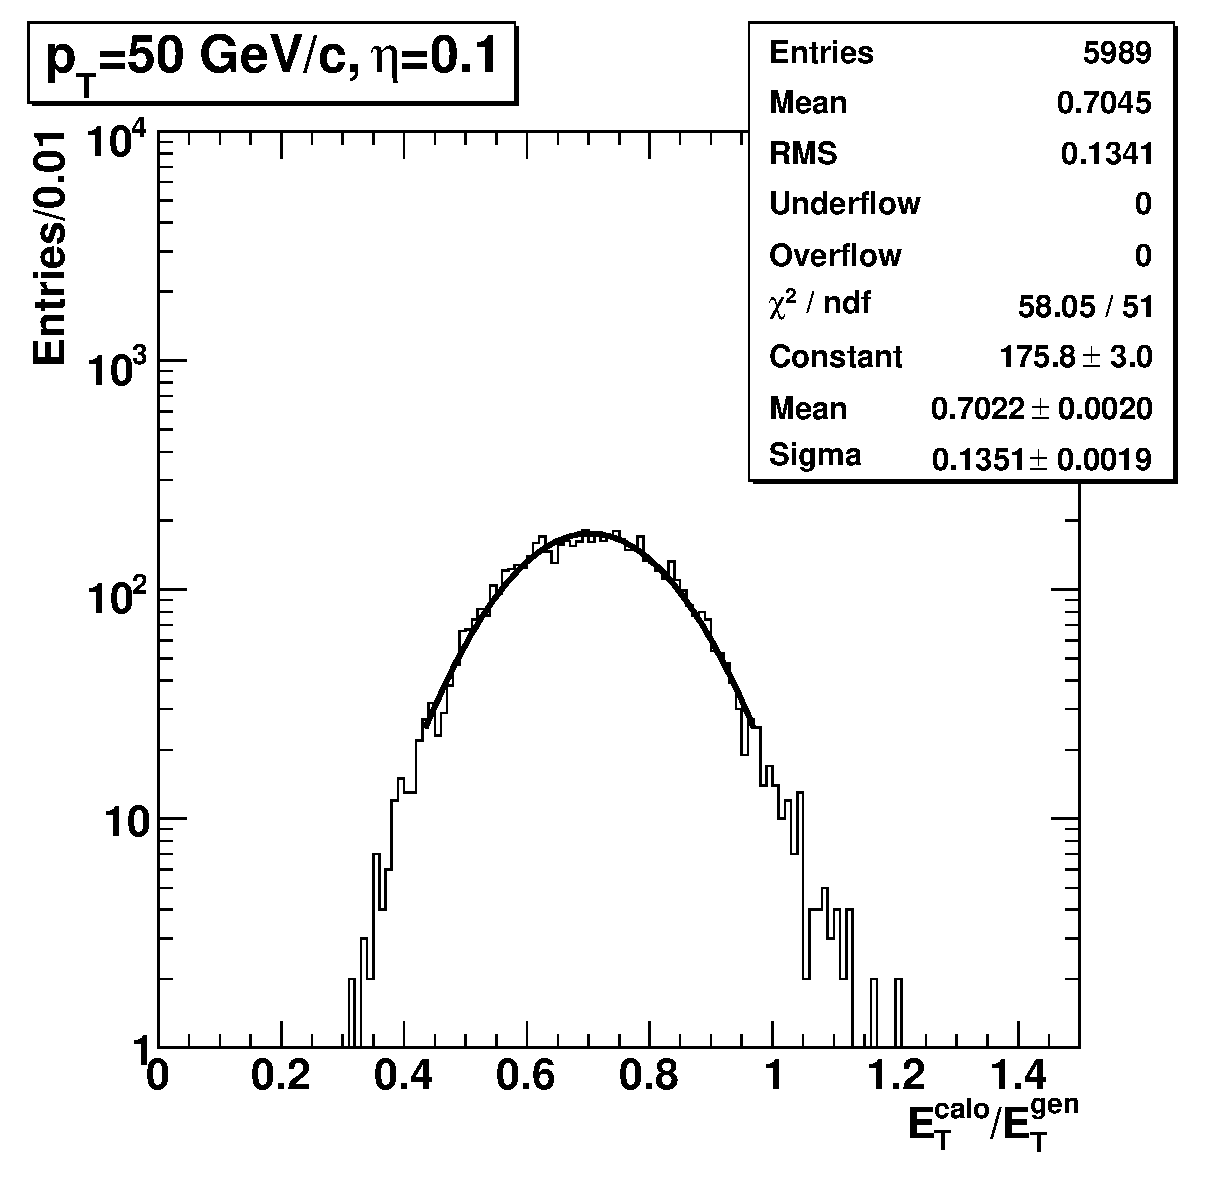
\includegraphics[width=0.31\textwidth]{fig/h_ETRatio_ET_py_fit_corr_eta0.1_pT50.eps} &
 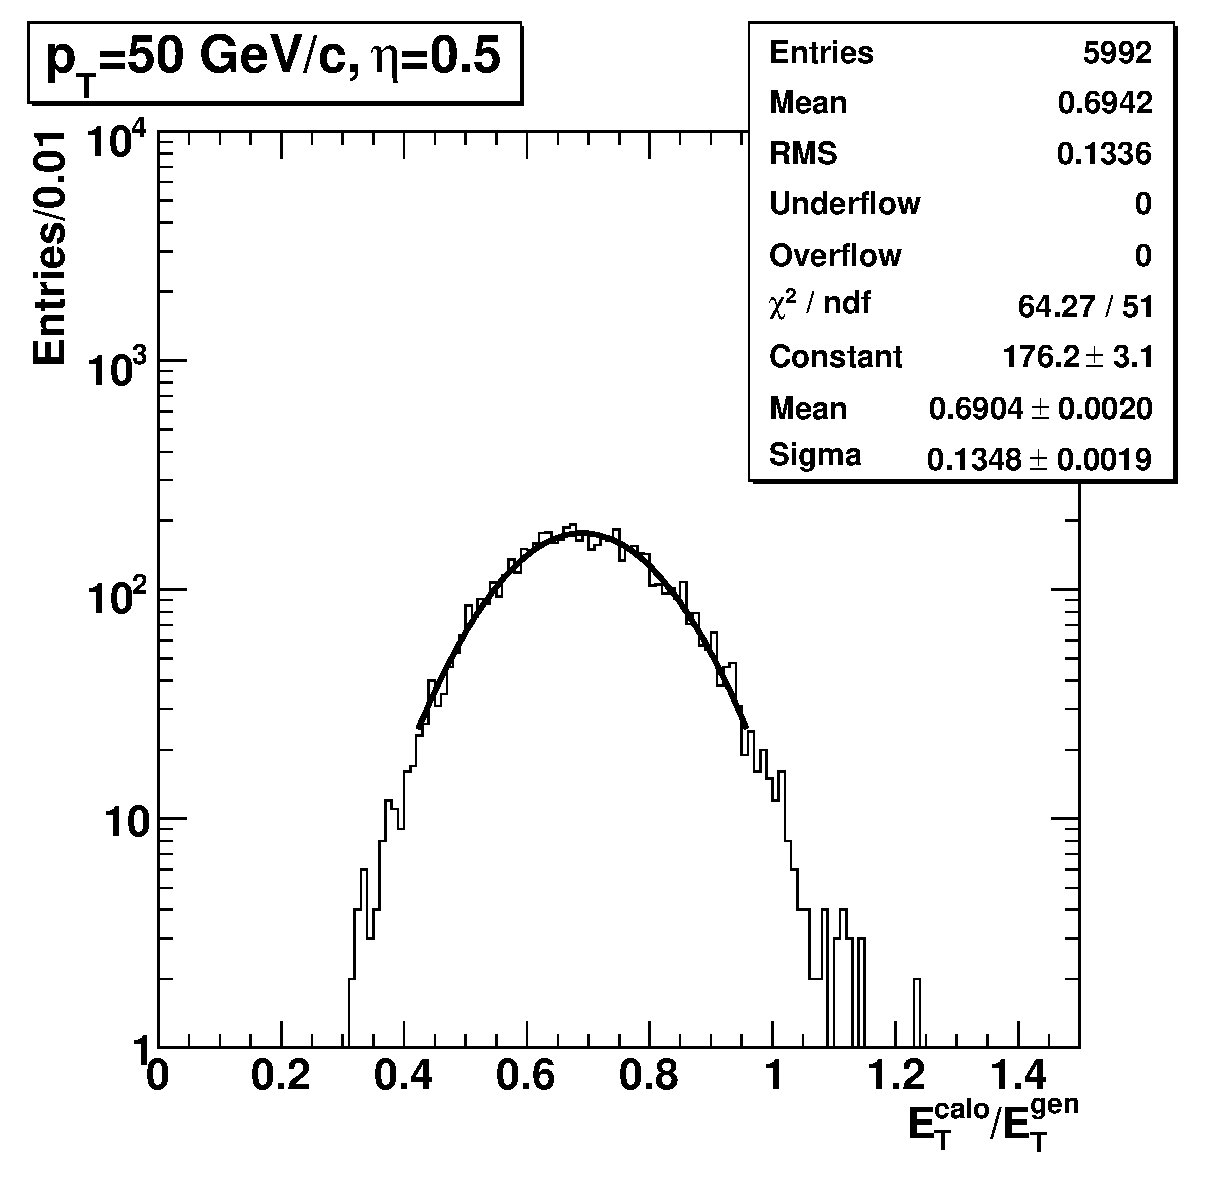
\includegraphics[width=0.31\textwidth]{fig/h_ETRatio_ET_py_fit_corr_eta0.5_pT50.eps} &
 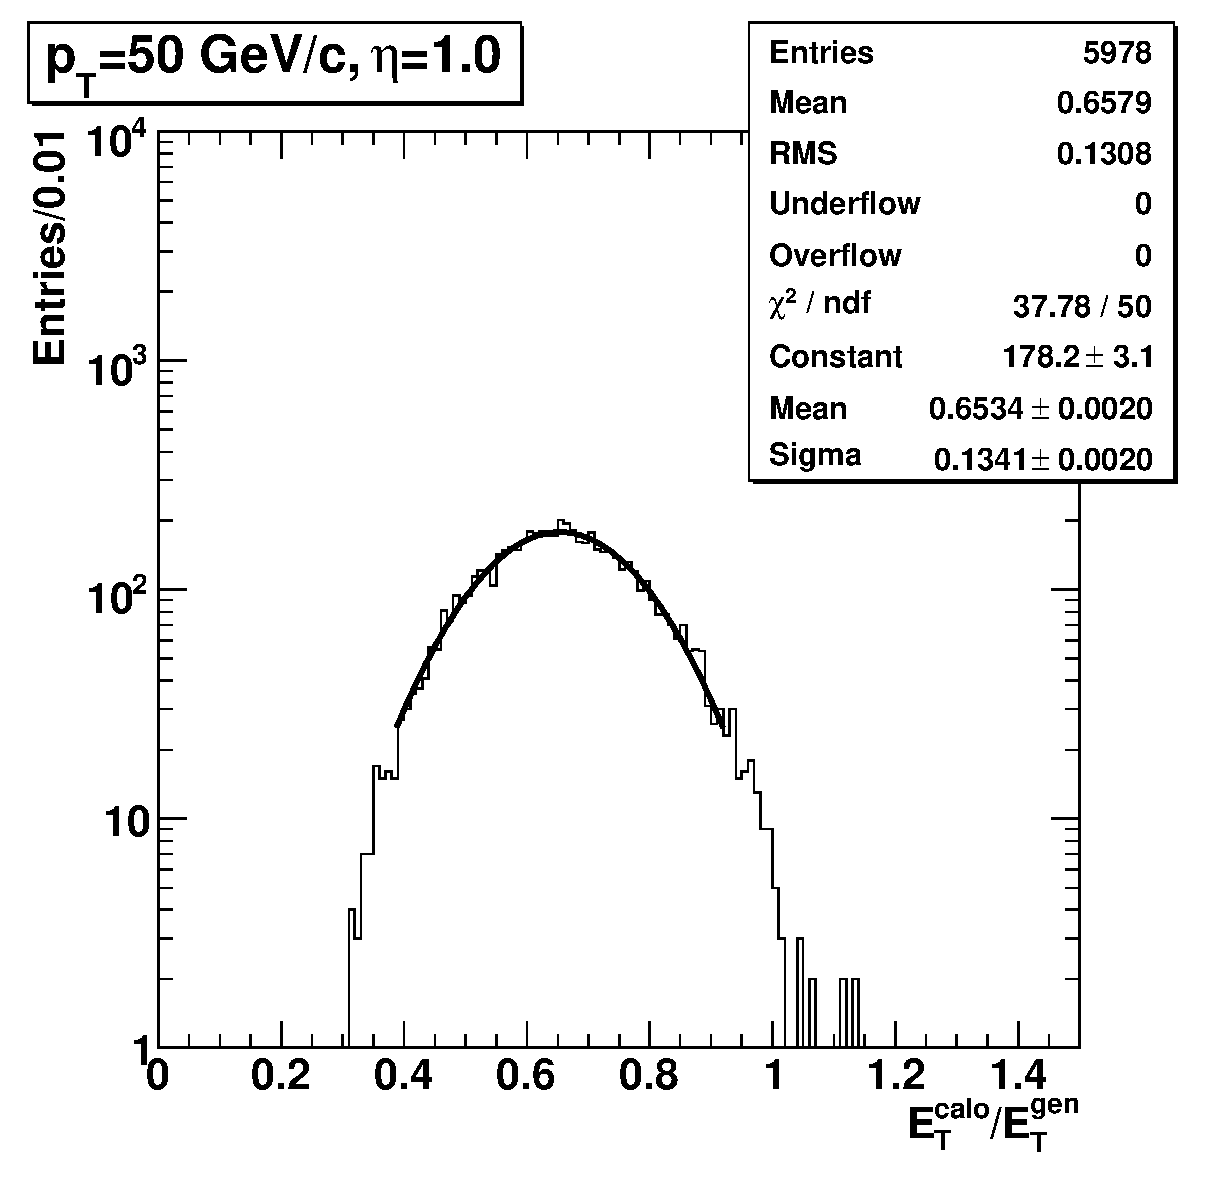
\includegraphics[width=0.31\textwidth]{fig/h_ETRatio_ET_py_fit_corr_eta1.0_pT50.eps} \\
\end{tabular}
\end{center}
\begin{center}
\begin{tabular}{lll}
 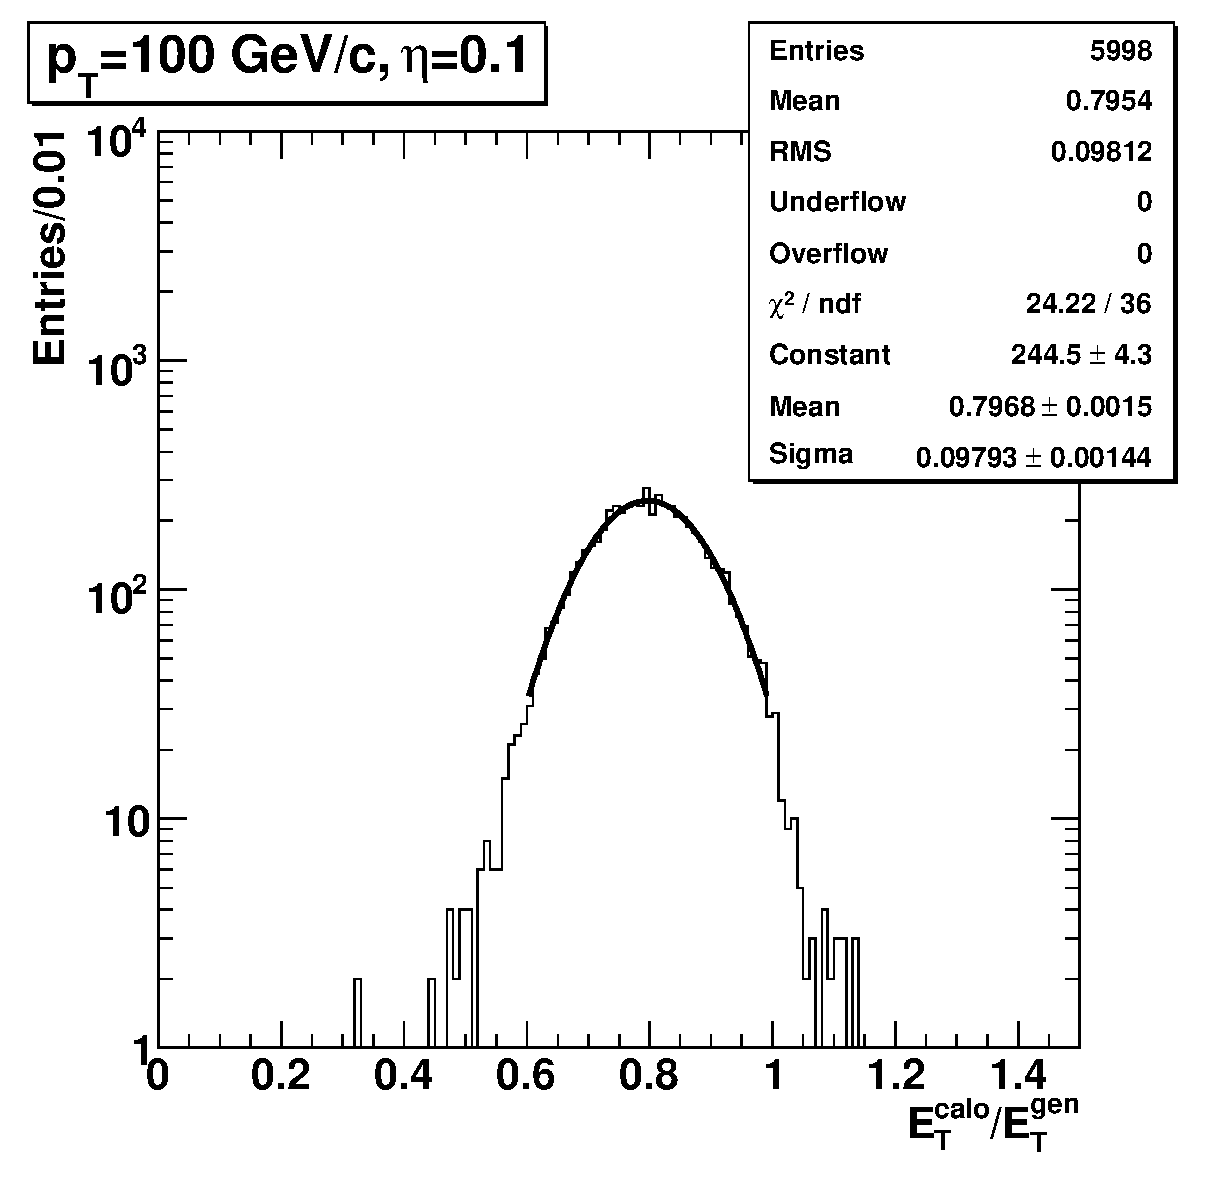
\includegraphics[width=0.31\textwidth]{fig/h_ETRatio_ET_py_fit_corr_eta0.1_pT100.eps} &
 \includegraphics[width=0.31\textwidth]{fig/h_ETRatio_ET_py_fit_corr_eta0.5_pT100.eps} &
 \includegraphics[width=0.31\textwidth]{fig/h_ETRatio_ET_py_fit_corr_eta1.0_pT100.eps} \\
\end{tabular}
\end{center}
\begin{center}
\begin{tabular}{lll}
 \includegraphics[width=0.31\textwidth]{fig/h_ETRatio_ET_py_fit_corr_eta0.1_pT300.eps} &
 \includegraphics[width=0.31\textwidth]{fig/h_ETRatio_ET_py_fit_corr_eta0.5_pT300.eps} &
 \includegraphics[width=0.31\textwidth]{fig/h_ETRatio_ET_py_fit_corr_eta1.0_pT300.eps} \\
\end{tabular}
\end{center}
\begin{center}
\begin{tabular}{lll}
 \includegraphics[width=0.31\textwidth]{fig/h_ETRatio_ET_py_fit_corr_eta0.1_pT500.eps} &
 \includegraphics[width=0.31\textwidth]{fig/h_ETRatio_ET_py_fit_corr_eta0.5_pT500.eps} &
 \includegraphics[width=0.31\textwidth]{fig/h_ETRatio_ET_py_fit_corr_eta1.0_pT500.eps} \\
\end{tabular}
\end{center}
\begin{center}
\begin{tabular}{lll}
 \includegraphics[width=0.31\textwidth]{fig/h_ETRatio_ET_py_fit_corr_eta0.1_pT1000.eps} &
 \includegraphics[width=0.31\textwidth]{fig/h_ETRatio_ET_py_fit_corr_eta0.5_pT1000.eps} &
 \includegraphics[width=0.31\textwidth]{fig/h_ETRatio_ET_py_fit_corr_eta1.0_pT1000.eps} \\
\end{tabular}
\end{center}
\begin{center}
\begin{tabular}{lll}
 \includegraphics[width=0.31\textwidth]{fig/h_ETRatio_ET_py_fit_corr_eta0.1_pT2000.eps} &
 \includegraphics[width=0.31\textwidth]{fig/h_ETRatio_ET_py_fit_corr_eta0.5_pT2000.eps} &
 \includegraphics[width=0.31\textwidth]{fig/h_ETRatio_ET_py_fit_corr_eta1.0_pT2000.eps} \\
\end{tabular}
\end{center}
\begin{center}
\begin{tabular}{lll}
 \includegraphics[width=0.31\textwidth]{fig/h_ETRatio_ET_py_fit_corr_eta0.1_pT4000.eps} &
 \includegraphics[width=0.31\textwidth]{fig/h_ETRatio_ET_py_fit_corr_eta0.5_pT4000.eps} &
 \includegraphics[width=0.31\textwidth]{fig/h_ETRatio_ET_py_fit_corr_eta1.0_pT4000.eps} \\
\end{tabular}
\end{center}
\begin{center}
\begin{tabular}{lll}
 \includegraphics[width=0.31\textwidth]{fig/h_ETRatio_ET_py_fit_corr_eta0.1_pT7000.eps} &
 \includegraphics[width=0.31\textwidth]{fig/h_ETRatio_ET_py_fit_corr_eta0.5_pT7000.eps} &
 \includegraphics[width=0.31\textwidth]{fig/h_ETRatio_ET_py_fit_corr_eta1.0_pT7000.eps} \\
\end{tabular}
\end{center}

\subsection{CaloJetsWithHO}

\begin{center}
\begin{tabular}{lll}
 \includegraphics[width=0.31\textwidth]{fig/h_ETRatioWithHO_ET_py_fit_corr_eta0.1_pT50.eps} &
 \includegraphics[width=0.31\textwidth]{fig/h_ETRatioWithHO_ET_py_fit_corr_eta0.5_pT50.eps} &
 \includegraphics[width=0.31\textwidth]{fig/h_ETRatioWithHO_ET_py_fit_corr_eta1.0_pT50.eps} \\
\end{tabular}
\end{center}
\begin{center}
\begin{tabular}{lll}
 \includegraphics[width=0.31\textwidth]{fig/h_ETRatioWithHO_ET_py_fit_corr_eta0.1_pT100.eps} &
 \includegraphics[width=0.31\textwidth]{fig/h_ETRatioWithHO_ET_py_fit_corr_eta0.5_pT100.eps} &
 \includegraphics[width=0.31\textwidth]{fig/h_ETRatioWithHO_ET_py_fit_corr_eta1.0_pT100.eps} \\
\end{tabular}
\end{center}
\begin{center}
\begin{tabular}{lll}
 \includegraphics[width=0.31\textwidth]{fig/h_ETRatioWithHO_ET_py_fit_corr_eta0.1_pT300.eps} &
 \includegraphics[width=0.31\textwidth]{fig/h_ETRatioWithHO_ET_py_fit_corr_eta0.5_pT300.eps} &
 \includegraphics[width=0.31\textwidth]{fig/h_ETRatioWithHO_ET_py_fit_corr_eta1.0_pT300.eps} \\
\end{tabular}
\end{center}
\begin{center}
\begin{tabular}{lll}
 \includegraphics[width=0.31\textwidth]{fig/h_ETRatioWithHO_ET_py_fit_corr_eta0.1_pT500.eps} &
 \includegraphics[width=0.31\textwidth]{fig/h_ETRatioWithHO_ET_py_fit_corr_eta0.5_pT500.eps} &
 \includegraphics[width=0.31\textwidth]{fig/h_ETRatioWithHO_ET_py_fit_corr_eta1.0_pT500.eps} \\
\end{tabular}
\end{center}
\begin{center}
\begin{tabular}{lll}
 \includegraphics[width=0.31\textwidth]{fig/h_ETRatioWithHO_ET_py_fit_corr_eta0.1_pT1000.eps} &
 \includegraphics[width=0.31\textwidth]{fig/h_ETRatioWithHO_ET_py_fit_corr_eta0.5_pT1000.eps} &
 \includegraphics[width=0.31\textwidth]{fig/h_ETRatioWithHO_ET_py_fit_corr_eta1.0_pT1000.eps} \\
\end{tabular}
\end{center}
\begin{center}
\begin{tabular}{lll}
 \includegraphics[width=0.31\textwidth]{fig/h_ETRatioWithHO_ET_py_fit_corr_eta0.1_pT2000.eps} &
 \includegraphics[width=0.31\textwidth]{fig/h_ETRatioWithHO_ET_py_fit_corr_eta0.5_pT2000.eps} &
 \includegraphics[width=0.31\textwidth]{fig/h_ETRatioWithHO_ET_py_fit_corr_eta1.0_pT2000.eps} \\
\end{tabular}
\end{center}
\begin{center}
\begin{tabular}{lll}
 \includegraphics[width=0.31\textwidth]{fig/h_ETRatioWithHO_ET_py_fit_corr_eta0.1_pT4000.eps} &
 \includegraphics[width=0.31\textwidth]{fig/h_ETRatioWithHO_ET_py_fit_corr_eta0.5_pT4000.eps} &
 \includegraphics[width=0.31\textwidth]{fig/h_ETRatioWithHO_ET_py_fit_corr_eta1.0_pT4000.eps} \\
\end{tabular}
\end{center}
\begin{center}
\begin{tabular}{lll}
 \includegraphics[width=0.31\textwidth]{fig/h_ETRatioWithHO_ET_py_fit_corr_eta0.1_pT7000.eps} &
 \includegraphics[width=0.31\textwidth]{fig/h_ETRatioWithHO_ET_py_fit_corr_eta0.5_pT7000.eps} &
 \includegraphics[width=0.31\textwidth]{fig/h_ETRatioWithHO_ET_py_fit_corr_eta1.0_pT7000.eps} \\
\end{tabular}
\end{center}


\section{Jet $\bE_\mathrm{T}$ Resolution vs. \texttt{hadEnergyInHO} Weight Factor}
\label{app:res_vs_weight}

\begin{center}
\begin{tabular}{lll}
 \includegraphics[width=0.31\textwidth]{fig/ET_res_vs_HO_wght_eta0.1_pT50.eps} &
 \includegraphics[width=0.31\textwidth]{fig/ET_res_vs_HO_wght_eta0.5_pT50.eps} &
 \includegraphics[width=0.31\textwidth]{fig/ET_res_vs_HO_wght_eta1.0_pT50.eps} \\
\end{tabular}
\end{center}
\begin{center}
\begin{tabular}{lll}
 \includegraphics[width=0.31\textwidth]{fig/ET_res_vs_HO_wght_eta0.1_pT100.eps} &
 \includegraphics[width=0.31\textwidth]{fig/ET_res_vs_HO_wght_eta0.5_pT100.eps} &
 \includegraphics[width=0.31\textwidth]{fig/ET_res_vs_HO_wght_eta1.0_pT100.eps} \\
\end{tabular}
\end{center}
\begin{center}
\begin{tabular}{lll}
 \includegraphics[width=0.31\textwidth]{fig/ET_res_vs_HO_wght_eta0.1_pT300.eps} &
 \includegraphics[width=0.31\textwidth]{fig/ET_res_vs_HO_wght_eta0.5_pT300.eps} &
 \includegraphics[width=0.31\textwidth]{fig/ET_res_vs_HO_wght_eta1.0_pT300.eps} \\
\end{tabular}
\end{center}
\begin{center}
\begin{tabular}{lll}
 \includegraphics[width=0.31\textwidth]{fig/ET_res_vs_HO_wght_eta0.1_pT500.eps} &
 \includegraphics[width=0.31\textwidth]{fig/ET_res_vs_HO_wght_eta0.5_pT500.eps} &
 \includegraphics[width=0.31\textwidth]{fig/ET_res_vs_HO_wght_eta1.0_pT500.eps} \\
\end{tabular}
\end{center}
\begin{center}
\begin{tabular}{lll}
 \includegraphics[width=0.31\textwidth]{fig/ET_res_vs_HO_wght_eta0.1_pT1000.eps} &
 \includegraphics[width=0.31\textwidth]{fig/ET_res_vs_HO_wght_eta0.5_pT1000.eps} &
 \includegraphics[width=0.31\textwidth]{fig/ET_res_vs_HO_wght_eta1.0_pT1000.eps} \\
\end{tabular}
\end{center}
\begin{center}
\begin{tabular}{lll}
 \includegraphics[width=0.31\textwidth]{fig/ET_res_vs_HO_wght_eta0.1_pT2000.eps} &
 \includegraphics[width=0.31\textwidth]{fig/ET_res_vs_HO_wght_eta0.5_pT2000.eps} &
 \includegraphics[width=0.31\textwidth]{fig/ET_res_vs_HO_wght_eta1.0_pT2000.eps} \\
\end{tabular}
\end{center}
\begin{center}
\begin{tabular}{lll}
 \includegraphics[width=0.31\textwidth]{fig/ET_res_vs_HO_wght_eta0.1_pT4000.eps} &
 \includegraphics[width=0.31\textwidth]{fig/ET_res_vs_HO_wght_eta0.5_pT4000.eps} &
 \includegraphics[width=0.31\textwidth]{fig/ET_res_vs_HO_wght_eta1.0_pT4000.eps} \\
\end{tabular}
\end{center}
\begin{center}
\begin{tabular}{lll}
 \includegraphics[width=0.31\textwidth]{fig/ET_res_vs_HO_wght_eta0.1_pT7000.eps} &
 \includegraphics[width=0.31\textwidth]{fig/ET_res_vs_HO_wght_eta0.5_pT7000.eps} &
 \includegraphics[width=0.31\textwidth]{fig/ET_res_vs_HO_wght_eta1.0_pT7000.eps} \\
\end{tabular}
\end{center}

\end{appendices}

\begin{thebibliography}{9}

\bibitem {ref:cms-jinst} The CMS Collaboration, S. Chatrchyan \textit{et al.}, ``The CMS Experiment at the CERN LHC'', 2008 JINST \textbf{3} S08004

\bibitem {ref:frontier} Global Tags for Conditions Data: \href{https://twiki.cern.ch/twiki/bin/view/CMS/SWGuideFrontierConditions}{https://twiki.cern.ch/twiki/bin/view/CMS/SWGuideFrontierConditions}

\bibitem {ref:cmssw} CMSSW Application Framework: \href{https://twiki.cern.ch/twiki/bin/view/CMS/WorkBookCMSSWFramework}{https://twiki.cern.ch/twiki/bin/view/CMS/WorkBookCMSSWFramework}

\bibitem {ref:scheme_b} R. Demina \textit{et al.}, ``Calorimeter Cell Energy Thresholds for Jet Reconstruction in CMS'', CMS NOTE 2006/020

\bibitem {ref:thresh} Z. Qi \textit{et al.}, ``HCAL Noise Thresholds in CMSSW\_2\_2\_3'', Jet Algorithms Meeting, Jan 15, 2009 \href{http://indico.cern.ch/getFile.py/access?contribId=1&resId=1&materialId=slides&confId=49768}{http://indico.cern.ch/getFile.py/access?contribId=1\&resId=1\&materialId=slides\&confId=49768}

\bibitem {ref:ecal_cell} C. Sander \textit{et al.}, ``$\slashed E_\mathrm{T}$ from Simulated Very High $p_\mathrm{T}$ Jets'', MET Working Group Meeting, Nov 21, 2008 \href{http://indico.cern.ch/getFile.py/access?contribId=2&resId=0&materialId=slides&confId=45919}{http://indico.cern.ch/getFile.py/access?contribId=2\&resId=0\&materialId=slides\&confId=45919}

\bibitem {ref:one_to_one} One-To-One Matching Tool: \href{https://twiki.cern.ch/twiki/bin/view/CMS/WorkBookJetAnalysis}{https://twiki.cern.ch/twiki/bin/view/CMS/WorkBookJetAnalysis}

\end{thebibliography}

\end{document}
